% Thesis!

% Two Column Format
\documentclass[12pt]{ucthesis}
%this allows us to specify sections to be single or multi column so that things like title page and table of contents are single column
\usepackage{listings}
\usepackage{placeins}
\usepackage{caption}
\usepackage{todonotes}
\usepackage{url}
\usepackage{graphicx}
\usepackage{amssymb}
\usepackage{amsmath}
\usepackage[letterpaper]{geometry}
\usepackage[overload]{textcase}
\usepackage{verbatim}

\usepackage{titlesec}

\definecolor{dkgreen}{rgb}{0,0.6,0}
\definecolor{gray}{rgb}{0.5,0.5,0.5}
\definecolor{mauve}{rgb}{0.58,0,0.82}

\lstdefinelanguage{JavaScript}{
  keywords={typeof, new, true, false, catch, function, return, null, catch, switch, var, if, in, while, do, else, case, break, this},
  keywordstyle=\color{blue}\bfseries,
  ndkeywords={class, export, boolean, throw, implements, import, this},
  ndkeywordstyle=\color{darkgray}\bfseries,
  identifierstyle=\color{black},
  sensitive=false,
  comment=[l]{//},
  morecomment=[s]{/*}{*/},
  commentstyle=\color{purple}\ttfamily,
  stringstyle=\color{red}\ttfamily,
  morestring=[b]',
  morestring=[b]"
}


\lstset{frame=tb,
  language=JavaScript,
  aboveskip=3mm,
  belowskip=3mm,
  showstringspaces=false,
  columns=flexible,
  basicstyle={\small\ttfamily},
  numbers=none,
  numberstyle=\tiny\color{gray},
  keywordstyle=\color{blue},
  commentstyle=\color{dkgreen},
  stringstyle=\color{mauve},
  breaklines=true,
  breakatwhitespace=true,
  tabsize=3
}

\newenvironment{Figure}
  {\par\medskip\noindent\minipage{\linewidth}}
  {\endminipage\par\medskip}

\titleformat{\chapter}[display]% NEW
    {\normalfont\centering}{\chaptertitlename\ \thechapter}{12pt}{}% NEW
\titlespacing*{\chapter}{0pt}{30pt}{20pt}% NEW

%\titleformat{\section}[block]{first}{label}{12pt}

\titleformat{\section}{}{\thesection}{1em}{}
\titleformat{\subsection}{}{\thesubsection}{1em}{}
\titleformat{\subsubsection}{}{\thesubsubsection}{1em}{}
\titleformat{\paragraph}{}{\theparagraph}{1em}{}

% \setcounter{secnumdepth}{5}
\setlength{\parindent}{0.25in} \setlength{\parskip}{6pt}

\geometry{verbose,nohead,tmargin=1.25in,bmargin=1in,lmargin=1.5in,rmargin=1.3in}

\setcounter{tocdepth}{3}

\graphicspath{ {./images/} }

% Different font in captions (single-spaced, bold) ------------
\newcommand{\captionfonts}{\small\bf\ssp}

\makeatletter  % Allow the use of @ in command names
\long\def\@makecaption#1#2{%
  \vskip\abovecaptionskip
  \sbox\@tempboxa{{\captionfonts #1: #2}}%
  \ifdim \wd\@tempboxa >\hsize
    {\captionfonts #1: #2\par}
  \else
    \hbox to\hsize{\hfil\box\@tempboxa\hfil}%
  \fi
  \vskip\belowcaptionskip}
\makeatother   % Cancel the effect of \makeatletter
% ---------------------------------------

\begin{document}

%%%%%%%%%%%%%%%%%%
%%% Cover Page %%%
%%%%%%%%%%%%%%%%%%

% A Survey of Web Testing Frameworks and Workflow for Testing JavaScript Applications, Developing A Workflow for new Web Developers, 
\title{Creating a Testing Framework and Workflow for Developers New to Web Application Engineering} %\vfill gives us the black space at the top of the page
\author{Taggart Ashby}
\degreemonth{June} \degreeyear{2014} \degree{Master of Science}
\defensemonth{June} \defenseyear{2014}
\numberofmembers{3} \chair{Michael Haungs, Ph.D.} \othermemberA{Franz Kurfess, Ph.D.} \othermemberB{David Janzen, Ph.D.} \field{Computer Science} \campus{San Luis Obispo}
\copyrightyears{seven}

\maketitle

\begin{frontmatter}

\copyrightpage

\committeemembershippage

%%%%%%%%%%%%%%%%
%%% Abstract 
%%% VERY General overview of problem and solution in paper
%%%%%%%%%%%%%%%%
\begin{abstract}
Web applications are quickly replacing standalone applications for everyday tasks. These web applications need to be tested to ensure proper functionality and reliability. There have been substantial efforts to create tools that assist with the testing of web applications, but there is no standard set of tools or a recommended workflow to ensure speed of development and strength of application.

We have used and outlined the merits of a number of existing testing tools and brought together the best among them to create what we feel is a fully-featured, easy to use, testing framework and workflow for web application development.

We then took an existing web application, PolyXpress, and augmented its development process to include our workflow suggestions in order to incorporate testing at all levels. PolyXpress is a web application that ``allows you to create location-based stories, build eTours, or create restaurant guides. It is the tool that will bring people to locations in order to entertain, educate, or provide amazing deals.''\cite{PX} After incorporating our testing procedures, we immediately detected previously unknown bugs in the software. In addition, there is now a workflow in place for future developers to use which will expedite their testing and development.
\end{abstract}

\tableofcontents

\end{frontmatter}

\pagestyle{plain}

\renewcommand{\baselinestretch}{1.66}

%%%%%%%%%%%%%%%%%%%%
%%% Introduction/Motivation
%%% More detailed, but still general, description of problem and why we want to solve it
%%%%%%%%%%%%%%%%%%%%
\chapter{Introduction}
Since the advent of the internet, the web has undergone an impressive evolution from plain-text webpages to the highly stylized and functional pages that we see today. In the last four to six years there has been an explosion of new web technologies that make applications more functional: HTML5, CSS3, WebGL, Touch APIs, Geo-location, and a host of others. \cite{EvolutionOfWeb} In that same time period, the number of global internet users has grown to somewhere around two and a half billion. \cite{EvolutionOfWeb} The combination of these new technologies and the ever-increasing usage of the internet has led to a significant growth in the number and complexity of web applications.

Like any piece of software, these web applications require testing in order to determine their correctness and give their users the best experience possible. Unfortunately, web applications are new and there are no standard practices for testing them. Their dynamic and distributed nature require a different testing toolkit than their predecessors. In addition, web applications are being produced in high volume and with quick development times, leading to a need for rapid testing.

We have found that this is not a solved problem by looking at some of the biggest web applications around. A 2011 study showed that YouTube has at least eight errors, Apple has at least seven, Microsoft at least four, and the list goes on. \cite{ErrorsInTheWild} That may seem like a incredibly small amount for such monoliths but every error is an opportunity for malfunction and customer dissatisfaction.

\section{What Already Exists}
Web developers are not clueless, they understand that there is a need for testing of web applications. Unfortunately, web development is still a relatively new domain and developers have not come together to work on the problem of testing but rather have come up with their own proprietary solutions in isolation or merely on a per-project basis. Some of these tools have gained traction and become larger, more general, tools.

Many of these tools are targeted at solving one or two aspects of complete testing but do not cover everything. In addition, some of the tools overlap or require tight coupling that prevents them from being used in combination with one another. Having to wade through a sea of similar tools or try to force tools to work together is time-consuming, which can be the death of a cutting-edge application. The more time an application is off the market, the more time competitors have to develop their own versions. Yet another problem is that deciding between similar tools can be discouraging to the developer that just wants to write their application and test it quickly.

Even the tools that already exist suffer from additional problems regarding their stages of development and amount of support. As will be discussed later, we've found tools that are in their beta stages that show incredible promise as well as mature tools that are widely used but leave much to be desired. These problems effect both industry tools as well as independent developers.

There needs to be a framework in place for testing these multi-layer, multi-faceted web applications that is easy to use, allows for quick development, and is thorough in its coverage. This thesis will explore some of the most popular tools with the end goal of gathering the best tools out there and collecting them in one place. We will attempt to gather tools that work well together and cover all aspects of testing for an average developer, particular a developer who has experience in some field of software but may be new to web applications. Our hope is that this thesis will serve as a starting point and guide to future web application developers.

\section{Problems Still Faced}
% - A lot of products to test against (browsers)
Testing web applications is difficult. The web offers an impressive set of features, but with those features come some draw-backs. Two of the most frustrating drawbacks for developers are the number of platforms and the web's asynchronous nature.

In the very beginning, web applications were easy to write and test because the only code was plain HTML with a common set of HTML tags. It did not matter what browser was used to view the content because the viewer was always a home computer rendering plain HTML. As time progressed, individual browsers began offering additional features and web applications became more rich but harder to test because the developer would need to run their code on multiple browsers to make sure they all behaved similarly. In today's technological world, it is nearly impossible to run one's web application on all of the possible browser versions, configurations, and platforms that are available. Web applications are on home computers, phones, tablets, MP3 players, refrigerators \cite{SamsungFridge}, and a variety of other devices of varying sizes and capabilities. As a developer, one wants to target as many of those platforms as possible with a single code-base to save time and effort. A naive developer might just release an application on all platforms and hope for the best, but releasing on all platforms without testing will likely drive consumers away if the application fails on their given platform.

% - Asynchronous shennanigans
The addition of JavaScript to web applications led to a golden age of feature-rich applications with exciting user interface (UI) features that had not before been seen. This set of features and UI improvements came with the complication of asynchronous execution. Unlike traditional multi-threaded software, however, the developer is not given access to individual threads, they only have access to the main thread. This sort of implementation is essential for dealing with asynchronous events like button clicks, loading data separately so as not to hold up the web page, and a variety of other niceties, but is a cause of major headaches in testing. Without access to individual threads, the developer has to either write synchronous code that will be slow and not user-friendly, or rely on other mechanisms that allow code to be sequenced. Often it is hard to get code properly sequenced and it requires changing straightforward functions to a hideous amalgamation of callbacks.

There is no overarching solution to these problems, but in order to understand the motivations behind this thesis, one must understand the problems facing web application developers.

\section{Contributions of This Thesis}
%- Framework
The goal of this thesis is to bring together tools that are already available for testing and combine them into a single framework that offers novice web application developers a toolkit for their testing needs. There are plenty of strong tools available and we hope to gather a subset of those tools to cover as much of the testing spectrum as possible. 

In addition to creating a single framework, we have set out to weigh the options between the most popular frameworks so that a developer can make informed decisions about the needs of their projects and substitute appropriate technologies. Since every project is unique, a single set of tools cannot possibly cover the gamut. In addition to the single set of recommendations, the most popular tools are discussed so that the developer is free to pick and choose as they see fit.
%- Wade through all the tools currently out there
%-- Focus in, no need to have every developer check out all 10000 tools
%-- Weigh options

%%%%%%%%%%%%%%%%%%
%%% Background 
%%% Information needed for reader to know what’s going on
%%% 	Server/Client Communication
%%% 	Cloud services
%%% 	Appropriate terms and definitions
%%%%%%%%%%%%%%%%%%
\chapter{Background}
To make the rest of the paper more understandable and to define the terms used in the remainder of the paper, we will outline the various concepts and technologies surrounding the web.
If one is familiar with HTML5, JavaScript, and Testing concepts and statistics, it will likely be safe to skip this background section.

\section{Web Application Strengths}
Web applications are great for both developers and consumers. They have a number of characteristics that make them more desirable than shrink-wrap software. These attributes include versioning, availability, platform independence, and the ability to rapidly prototype.

\subsection{Versioning}
Web applications can be updated at any time with instant roll-out and feedback. It requires absolutely no user interaction because the web page always serves the latest resources. In comparison to something like Microsoft Office that requires users to manually update, this feature leads to applications that can address problems quickly, roll-out security updates instantly, and incorporate consumer feedback much more often than any other type of software. For example, Google Docs is becoming incredibly popular as an online document editing suite. Updates to Google Docs are rolled out frequently and require little to no input from the user. Another perk is that users are not given a choice. This can lead to occasional customer outrage, but more often than not it is a powerful gain for both feature improvement and application security. There is no need to support legacy systems that may contain serious bugs.

\subsection{Availability}
Web applications are available anywhere there's internet\footnote{A recent push in the web application community is toward offline versions of applications that merely cache changes until the user can connect to the internet once again and all changes are pushed online. This increases the availability of web applications even further.}. There is rarely need to install anything on a given device. Due to the ever-increasing popularity of mobile devices, most applications have both mobile and full versions of their software and so the application is ``with'' the user at all times. This instant and continuous availability means that users only have to know how to use a web browser in order to access the application.

\subsection{Multi-platform}
Very similar to the availability strength, web applications are platform independent. Whether the user is on their phone, tablet, laptop, or PC, the application only requires a web browser with certain functionality. Nearly all devices made today come equipped with browsers that support the necessary functionality. This also means that the developer need not, generally, worry about hardware configurations, conflicting software, and other problems that can arise in desktop applications. 

The developer is not free from all worry as they must still consider differing web browsers. This problem, however, is almost fully remedied by a number of online APIs, such as jQuery\cite{jQuery}, that will rework underlying code based on browser versions and types. 

\subsection{Rapid Prototyping}
Web applications are fantastic for rapid prototyping because of all of the strengths discussed above. An idea can be prototyped and posted on a website quickly and rapid iteration can occur without the user even necessarily noticing. There are a number of web tools that will record where users are clicking, what features they're using, how long they're spending on a given page or step of a process, and a number of other metrics that can make iterations more directed and effective.

\section{Web Features}
Here we'll discuss some of the prevalent technologies that recently appeared in web applications and development. By no means is this an exhaustive list, just a sampling of the more prominent ones.

\subsection{HTML5}
The latest revision of HTML is HTML5 which first debuted on Firefox back in 2009. \cite{EvolutionOfWeb} HTML5 has not been officially recommended by the W3C (World Wide Web Consortium) who is the official keeper and recommender of web standards, however, there is a plan for final recommendation this year, 2014, called Plan 2014. \cite{Plan2014} What this means is that in 2014 the W3C will release a stable HTML5 Recommendation which will make HTML5 an official standard and help universalize all the separate implementations.

The HTML5 specification brings with it a number of new features including: audio and video tags, the canvas element, drag-and-drop functionality, web storage, offline page support, and a number of other modern web features. A lot of HTML5's features revolve around the inclusion of multimedia in web pages and stronger graphical processing and programming. HTML5 is a collection of new HTML elements and markup as well as libraries written in Javascript.

As the web is being increasingly used on mobile devices, HTML5 also introduces geolocation functionality. This functionality requires user approval, but once that approval is gained, the web application has access to a rough area in which the user is located. When used on devices that have GPS, such as phones and tablets, this area is more defined and the user's position can be obtained more reliably and accurately. This geolocation functionality has opened the door for brand new types of web applications that can more closely tie in with what the user is seeing or the area that they are in. For example, advertisements can be more targeted or an application can display distances to nearby points of interest.

JavaScript, though not the only scripting language with web use, is the primary language used to compliment HTML5 when making web applications. It is an interpreted language that is most often associated with client-side functionality, but in recent times has extended to the server-side. JavaScript is a prototype based object oriented scripting language with dynamic typing and first-class functions. Much of JavaScript's popularity stems from this dynamic nature that allows for quick, and often dirty, implementation of features in an iterative environment.

\subsection{Node.JS}
As a quick aside, it will be useful to have information about Node.JS as it is used in the sample application and the evaluation application. Node.JS, often called simply Node, is a JavaScript API for creating and running servers. ``Node's goal is to provide an easy way to build scalable network programs.'' \cite{Node} Node was created in 2009 and is sponsored by Joyent. Node does not use thread-based networking, instead opting for a single-threaded event loop and non-blocking I/O. Node allows developers to create and control web servers without the need for external software, such as Apache, commonly found in other sites.

Node is found in a number of popular sites including: PayPal, The New York Times, Yahoo!, Uber, LinkedIn, Microsoft Azure, and a number of others. \cite{Node}

One of the biggest draws of Node.js is the ability to write all of one's code, client and server, in a single programming language, Javascript. This leads to better understanding of the codebase as well as the opportunity for code reuse between client and server.

\section{Client/Server Architecture}
By their nature, web applications are distributed; they have a client-side and a server-side.

Here we'll discuss what the client-side is and does, what the server-side is and does, and how they communicate.

\subsection{Client-side}
First, we'll address what a client is. The simple answer is: The User. The User's phone, computer, tablet, or other device communicating with a given website or application is the client. More specifically, the browser or service being using to communicate with the web is the client. 

The client-side portion of an application interacts with the browser to request assets from the server and then displaying them in a human-readable way. The client-side also deals with the user interface and interactivity of a web page, e.g., the client-side displays a web form, the client fills in the information and clicks ``submit'' and the client-side packages up the data and sends it to the server.

Client-side programming is done in a language that the browser understands, most frequently JavaScript. Though not technically programming languages, client-side programming is also done through HTML and CSS which control the look and feel of web pages.

\subsection{Server-side}
A server is the entity, be it machine, person, or cloud service, that stores the information about a given web page or application. The server stores all assets: HTML pages, images, videos, databases, etc, and provides them upon request to the client. The server also handles all of the processing for interactivity, accounts, and general number-crunching.

\subsection{Client and Server Interactions}
The client has limited access to resources on any given web application. This access is restricted by the server. Without such restrictions in place, someone could access user databases, credit card information, order reports, etc. In addition, there would be an overwhelming amount of content for a client to parse through, even if they have no malicious intent.

Clients communicate with the Server through a request-response architecture. Clients send a request to the server, often with information attached, such as a form submittal or login, and the server returns a response with either a success/failure message, or additional data.

One example of a client-server architecture that is popular for the web is the Representational State Transfer, also known as REST, architecture. If a client-server architecture meets all of the REST criteria, it is said to be RESTful. As this paper is not about Client Server interactions, we will not outline the constraints but instead outline how RESTful APIs look in web applications. The RESTful web APIs use: 1) a base URI, 2) an internet media type, and 3) the standard HTTP methods.

A base URI is simple; in the context of a web application, it is just a URL such as ``http://myrestapi.com/entities''.

An internet media type is a way to represent and store data that may need to be sent with a request going either direction, from client to server or server to client. Most web APIs use JavaScript Object Notation, known as JSON, to store data.

The standard HTTP methods are GET, PUT, POST, and DELETE. These methods define what the request is intending to do. For example, a GET request sent to ``http://myrestapi.com/entities'' would indicate to the server that the client wants to get information regarding all entities. A PUT request would indicate that the client wishes to replace the entire entity collection with another collection that would be sent along with the request. A POST request would ask the server to create a new entity in the collection. Finally, a DELETE request would tell the server to delete the entities. The four methods take on slightly different, but very similar meanings when used with specific element URIs, such as ``http://myrestapi.com/entities/entity1''. A GET request asks the server for a displayable version of the entity and the client then displays it. A PUT request asks the server to replace the existing entity or create an entire new entity if one does not exist. A POST request is generally not used as that implies that this single entity is itself a collection. A DELETE request asks the server to remove this entity.

An important part of being a RESTful API is that any change to a web page or element is done through a hypertext link and all actions on an element share a single URI. For example, all updates to ``entity1'' are done through ``http://myrestapi.com/entities/entity1'' using the various HTTP methods that can be called using hypertext links on the page. Compare this to a different way to handle that functionality such as ``http://myrestapi.com/entities/UpdateEntity'' where the HTTP request contains information regarding the entity to update. This method handles all updates, regardless of which entity is changing, through a single URI.

\section{Defining Testing}
IEEE defines software testing as ``the dynamic verification of the behavior of a program on a finite set of test cases, suitably selected from the usually infinite executions domain, against the expected behavior.'' \cite{TestingDefinition} Put a bit more simply, software testing is the process of making sure the program does what it is supposed to.

There are a number of different types of tests and testing concepts. We will focus on Unit Testing, Integration Testing, Continuous Integration, and Acceptance Testing.

\subsection{Unit Testing}
Unit testing is the testing of specific functions and functionality, or ``test units.'' According to IEEE, test units are ``[a] set of one or more computer program modules together with associated control data, [...] usage procedures, and operating procedures that satisfy the following conditions: 1) All modules are from a single computer program. 2) At least one of the new or changed modules in the set has not completed the unit test. 3) The set of modules together with its associated data and procedures are the sole object of a testing process.''\cite{UnitTestDefinition} Generally this means the testing of individual functions but can extend to a set of functions that produce a single module of functionality. What sets Unit Testing apart from other types of testing is that tests focus on one portion of the code or system rather than interactions between modules or the entire system.

Here's a brief example:
\begin{lstlisting}
function Word(startingWord) {
  this.makePlural = function () { ... }
  this.pastTense = function () { ... }
  this.partOfSpeech = function () { ... }
}

function Sentence(listOfWords) {
  this.listOfWords = listOfWords;
  this.isGrammaticallySound = function () { ... }
  this.wordCount = function () {
    return this.listOfWords.length();
  }
  this.makePastTense = function () { ... }
  this.pluralize = function () { ... }
}

// Word Tests
function testMakePluralWord() { // Unit Test
  var myWord = new Word("cheese");
  myWord.makePlural();
  assert(myWord == "cheeses");
}

function testPastTense () { ... } // Unit Test
function testPartOfSpeech () { ... } // Unit Test

function testMakePluralCheckPartOfSpeech () { ... } // Not a Unit test, testing multiple units

// Sentence Tests
function testWordCount () { // Unit Test, no Word-specific functionality called
  var myWords = [new Word("hello"), new Word("world"), new Word("cheese")];
  var mySentence = new Sentence(myWords);

  assert(mySentence.wordCount == 3);
}

function testPluralize () { ... } // Integration Test, not Unit Test, would need to use Word.makePlural
function testIsGrammaticallySound () { ... } // Another Integration Test, would need to call Word.partOfSpeech

\end{lstlisting}

In the above example there are two modules, \lstinline{Word} and \lstinline{Sentence}. Unit Testing the \lstinline{Word} is relatively simple because it is self-contained and only runs functions on the string given to it. Unit Testing the \lstinline{Sentence} module is tougher because of its reliance on \lstinline{Word}s. The goal of a good set of Unit Tests is to test as much of a module as possible in isolation from all other modules. This includes interactions between modules. In our example, testing the \lstinline{wordCount} function is a Unit Test because none of the \lstinline{Word} functionality is actually required. The other methods of \lstinline{Sentence} pose a problem because of their need to call \lstinline{Word} functions. Although there are ways to Unit Test those functions, that is beyond the scope of this overview and would only serve to confuse the reader.

Unit tests are important because they are done in isolation from one another. The purpose of a unit test is to ensure that once individual modules are put together, the developer need only focus on the interaction between them instead of their individual functionality. Without the assurances of prior unit tests, integration would be a more stressful and mysterious proposition.

\subsection{Integration Testing}
After writing Unit tests, a developer writes Integration tests. Integration tests are used to determine if modules work together to produce correct results. In our previous example, this would mean testing most of the \lstinline{Sentence} functions to ensure that they properly use the \lstinline{Word}s that the \lstinline{Sentence} contains. Integration Tests cover a wider variety of test situations from single methods to entire modules.

Integration Testing is important because it gives the developer a sense of what modules are actually producing correct results, as opposed to which modules are functioning as anticipated. This distinction is critical to make. Unit Tests ensure that individual modules function. Integration tests are usually written in a way that is close to how they will actually be used in the final product, giving the developer a sense of which features are working and which are not.

\subsection{Continuous Integration}
The original definition of Continuous Integration involves the idea of developers committing from their  branches to a master branch daily so that changes are continuously integrated in an effort to make sure all branches can, in fact, be integrated. It has since evolved into a more general idea of a tool that runs commands after each commit to a repository. These commands generally encompass running unit tests, integration tests, user interface tests, and also often publishing and disseminating notifications to interested parties. This is invaluable feedback because the developer can see if they're making progress in the right direction as they write code, as opposed to a situation in which the developer finishes coding and finds out they've made a bad assumption or decision between this commit and the last. 

One of the most important aspects of a good piece of CI software is that it is automatic. There should be no need for a developer to do anything besides, perhaps, ``turn it on'' and start coding. As soon as a tool, CI or otherwise, requires more than one or two interactions to run, it becomes more of a nuisance and less of an asset.

\subsection{Acceptance Testing}
Acceptance testing is testing to confirm that the product meets a certain specification. Often this is making sure that the software meets an SRS (Software Requirements Specification) or a customer's outlined expectations. Often this testing is performed by the user of the software or customer that ordered the software, rather than the developers.

In an effort to automate this, some developers create ``User Stories'' which are automated tests that run a series of functions described by customers or an SRS. These User Stories are often written in a separate language that is more like English than code. The traditional User Story template is: ``As a \textless role\textgreater, I want \textless goal/desire\textgreater \space so that \textless benefit\textgreater.'' For example: ``As a supervisor, I want to find my employees by their employee ID.'' These user stories are then broken down into more specific steps that can be automated.

\subsection{Testing Statistics}
It is widely accepted that the earlier a developer detects a defect, the easier it is to fix that defect. A famous book, ``Code Complete'' by Steve McConnell \cite{DefectPic}, includes the following figure, showing this statistic on a rough graph.

\begin{Figure}
  \centering
	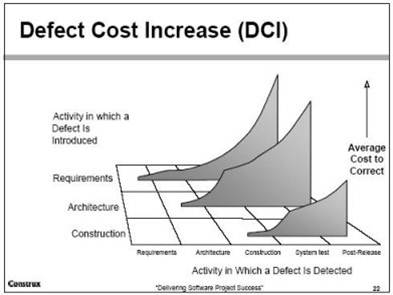
\includegraphics[width=0.75\linewidth]{defectcost.jpg} 
	\captionof{figure}{Illustration relating phase bug found in with effort required to fix.}
\end{Figure}

What we see here is that the earlier a defect is introduced the more it costs to fix it later. Of particular note is that the costs are roughly exponential, not linear. It's relatively easy to fix a bug that was introduced in the same stage that it is found, e.g. introducing a coding bug during ``Construction'' and fixing it while still writing code, prior to the ``System Test'' phase. The longer a bug lies undetected, the increasingly harder it becomes to fix that bug. 

% - CONSIDER REMOVING ALTOGETHER
% \subsection{Why Testing is Important}
% We're consistently surprised by how few people take testing seriously when it comes to non-trivial applications. Many developers will leave testing to their users, i.e., wait for users to have problems and report them before developers will fix them. This is an issue for a number of reasons, a few of which are: frustrated customers are unlikely to continue using a buggy product and are dissuaded from buying future products from the same developer, certain bugs can be security loopholes that may allow users access to information they shouldn't have, in the worst cases a bug may cause damage to a person or property and the developers would be on the hook.


%%%%%%%%%%%%%%%%%%%%%%
%%% Sample App 
%%%   Talk about test app
%%%%%%%%%%%%%%%%%%%%%%
\chapter{Testing Frameworks Survey}
In the following chapter we will discuss the testing frameworks that we looked at and the application we used to evaluate them. This chapter will conclude with a set of decision matrices outlining the strengths of each individual framework and where they overlap.

\section{ToDo Application}
In order to evaluate the various frameworks that we found online, we needed a small application with some functionality, but without the inherent complexity that was going to come with our final evaluation application. We chose a ToDo application made with Express.js, Node.js, and MongoDB.\cite{ToDoAppHomePage} Our choice of this application comes from its limited functionality and the ease of understanding the interactions that take place within the application, i.e. adding tasks to a ToDo list, marking tasks as completed, and viewing completed tasks. Here is a brief preview of the application's UI:

\begin{Figure}
  \centering
  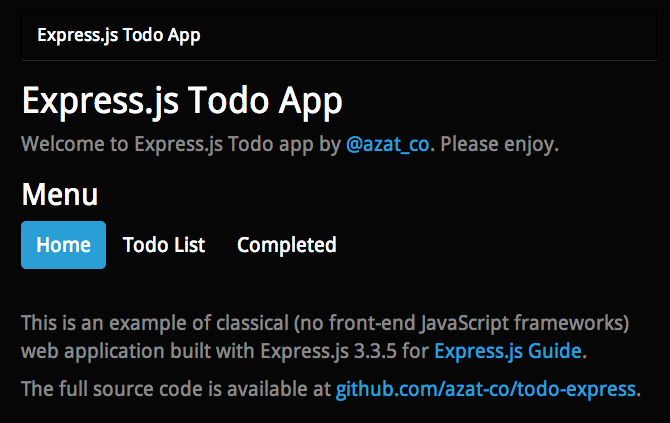
\includegraphics[width=0.75\linewidth]{todo_home.png}
  
\captionof{figure}{ToDo app home page, simple three-button naviagation}
  
\end{Figure}

\begin{Figure}
  \centering
  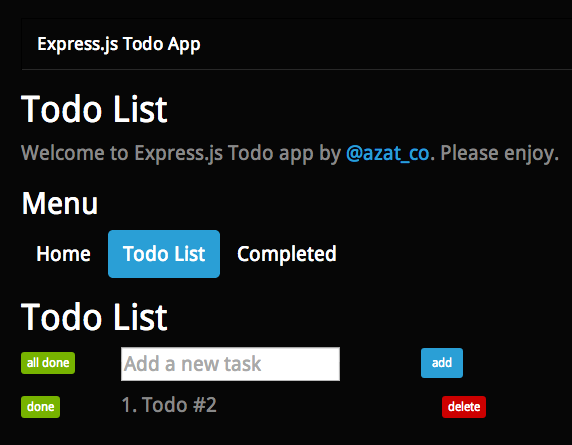
\includegraphics[width=0.75\linewidth]{todo_some_tasks.png}
  
\captionof{figure}{ToDo app task page}
  
\end{Figure}

\begin{Figure}
  \centering
  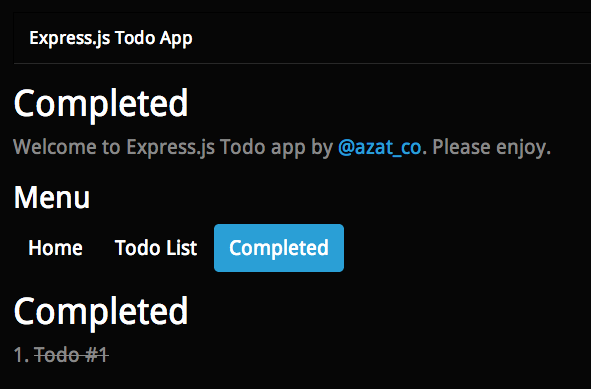
\includegraphics[width=0.75\linewidth]{todo_completed.png}
  
\captionof{figure}{ToDo app completed tasks page}

\end{Figure}

In addition to the simplicity and ease of understanding, this application was selected because it included Node.js and MongoDB as we wanted to see if the tools would be able to handle our final evaluation application which also uses those two.

One of the challenges in testing that we quickly came across was the asynchronous nature of the MongoDB function calls. As many web applications feature asynchronous calls, we will be discussing how the following frameworks deal with asynchronous test support.

\subsection{The Average Web Application}
In an effort to create a detailed and in-depth workflow and collection of tools, we have chosen to focus on web applications that use Node.js, JavaScript, and a backing Database. Although this will not cover all web application configurations, we wanted to narrow our scope in order to provide a specific, instead of general, set of guidelines and workflow suggestions.

Node.js is in wide use and because it is written in JavaScript we were able to test our client and server code using the same frameworks. Node.js also offers an incredible package manager, NPM, that allows for a smooth and efficient workflow.

JavaScript is the language of HTML5 and Node.js. It is used in over 87\% of all websites\cite{JSUsage} and as such allows us to create a workflow to cover a majority of web applications.

Many websites use databases to store user records, items in stock, and a number of other pieces of information. We wanted to make sure that the testing frameworks could support database functionality as it is often pivotal in running web applications.

\subsection{Tool Requirements}
Our requirements for the selection of testing tools was relatively simple. In addition to meeting the requirements of our ``average web application'', the only other requirement was that the tool was free. What ``free'' means is that the developer would have access to at least the minimum functionality needed to use the tool on \emph{one} application that is \emph{open-source}. What we quickly found is that web testing tools support open-source projects for free but are far less willing to provide free functionality to private or closed-source projects. 

Occasionally the cost of tools will be discussed but in general we did not review tools that only offered paid options.

\section{Unit Testing Frameworks}
The following frameworks are reviewed in chronological order of our evaluation. As such, comparisons will generally only be drawn between a framework and its predecessors in paper order. After all of the frameworks are outlined and evaluated, a section regarding the final decision will be made where comparisons will be drawn between all of them. 

Web applications can be broken down into two general parts. There is functionality behind the scenes that drives the web page and there is the user interface of the web page that conveys the information to the user. Unit testing frameworks are aimed at the functionality the drives the web page, not what the user sees.

\subsection{Jasmine}
The first of the unit testing frameworks that we looked at was Jasmine\cite{Jasmine}, a Behavior Driven Development (BDD) testing framework. BDD is based on Test Driven Development and adds some simplifications and patterns that attempt to bring both developers and businessmen into the software testing process. The idea behind Behavior Driven Development is that input from non-technical stakeholders as well as technical stakeholders can come together so that everyone understands what the project should do.

This relates to Jasmine is the way that the developer writes Jasmine tests. The idea behind jasmine tests is that they read, as much as possible, like English sentences. As an example, the following is a valid Jasmine test:
\begin{lstlisting}
describe("Arithmetic Test", function () {
  it("should compute the addition of two numbers", function () {
    expect(1 + 2).toEqual(3);
  });

  it("should be able to subtract numbers", function () {
    var theAnswer = 10;
    expect(12 - 2).toEqual(theAnswer);
  });
});
\end{lstlisting}
The \lstinline{describe} statement creates a test suite to organize related tests. Each \lstinline{it} statement is generally one test with some number of \lstinline{expect} statements. The above code is quite readable even to someone with no coding experience.

The default Jasmine did not support Node.js but there was a package available through npm called jasmine-node \cite{JasmineNode} that gave jasmine access to the node package and functions. 

Asynchronous testing using Jasmine is a bit of a chore because it requires a series of functions that are not straightforward. The asynchronous support comes in the form of a three-set function progression. The first function, \lstinline!runs(function () { .... })!, runs the asynchronous code. The second function, \lstinline!waitsFor(function () { ... })!, waits for a true value from a flag or other system. Finally, the third function, another \lstinline{runs(...)}, houses the assertions to determine if the code ran properly or not. These functions will be outlined in an example below. This method of asynchronous testing requires a fairly substantial amount of typing as well as complicated function chains when more than one asynchronous call is required.

\begin{lstlisting}
describe("Asynchronous specs", function() {
  var value, flag;

  it("should support async execution", function() {
    runs(function() {
      flag = false;
      value = 0;

      // Create an asynchronous function to run in half a second
      setTimeout(function() {
        flag = true;
      }, 500);
    });

    waitsFor(function() {
      value++;
      return flag;
    }, "The Value should be incremented", 750);

    runs(function() {
      expect(value).toBeGreaterThan(0);
    });
  });
});
\end{lstlisting}

The above test merely sets the \lstinline{flag} to true after half of a second, thus fulfilling the \lstinline{waitsFor} function and finally the assertions are run in the final \lstinline{runs} function.

Jasmine's BDD testing is something that we'd not see before. Having come from a more structured and developer-oriented testing background, it was interesting to see assertions and tests written in this different manner. The idea behind writing tests in this style is that requirements and customer feedback can be more easily translated into tests or even written by customers or other non-technical stakeholders. Jasmine does have asynchronous support but the three-function system is a bit tedious.

\subsection{Mocha}
Mocha\cite{Mocha} is another BDD testing framework that is almost identical to Jasmine. Unlike Jasmine, however, Mocha is not completely self-contained and requires an additional assertion library of one's choosing. We will outline our choice of Chai.js below.

Mocha, by default, also uses the \lstinline{describe -> it("should..."} pattern to create tests. Mocha offers a variety of other test interfaces for developers to write their test code. A few of the testing interfaces are outlined here:
\begin{lstlisting}
// BDD (default)
describe('BDD Suite', function () {
  it('should be test 1', function () {
    ...
  });
});

// TDD
suite('TDD Suite', function () {
  test('test 1', function () {
    ...
  });
));

// Exports
module.exports = {
  'Exports Suite': {
    'test 1': function () {
      ...
    }
  }
};

// QUnit
suite('QUnit Suite');
test('test 1', function () {
  ...
});

// Require, allows the developer to structure and call tests what they want
var testCase = require('mocha').describe

testCase('Require Suite', function(){
  testCase('test 1', function(){
    ...
  });
});
\end{lstlisting}
The developer doesn't gain anything by using one interface over another except the ability to write tests in a way that makes sense to them. There is no standard for writing assertions, as each assertion library is likely to be slightly different.

Mocha's approach to asynchronous testing is quite a bit more straightforward than Jasmine's. In the \lstinline{it(...)} anonymous function, there is an additional parameter called \lstinline{done} which is then called when the asynchronous call has finished. This required us to edit the code we were testing to make all the asynchronous calls accept an additional callback, but it was a very small price to pay for extended testability. An example asynchronous test would look like this:
\begin{lstlisting}
describe("Asynch Mocha Test", function () {
  it("looks like this", function (done) {
    myAsyncCall(param1, param2, function () { 
      // This callback expected to run when myAsyncCall finishes
      // Test ...
      // Test ...
      // ...
      done();
    });
  });
});
\end{lstlisting}

Overall Mocha offered more flexibility and better asynchronous support at the cost of additional setup. This increased flexibility came in the way of being able to select a testing interface and assertion library so that tests could be written in the way a developer wants. The cost of the flexibilty was the need to find an assertion library among the dozen that are out there. We prefer Mocha's method of asynchronous testing because it required considerably less typing on our part and was more easy to follow and read than the Jasmine chain of method calls.

\subsubsection{Chai.js}
For the assertion library we chose Chai.js\cite{Chaijs}. It contains three different assertion APIs: an Expect API, a Should API, and a more general Assert API. The Expect API provides assertions of the form \lstinline{expect(myVar).to.equal(10);} or \lstinline{expect(myArr).to.have.length(10);}. The Should API has assertions of the form \lstinline{myVar.should.be.a('number');} or \lstinline{myArr.should.have.length(10);}. Finally, the Assert API has the more tried and true \lstinline{assert.equal(myVar, 10);} and \lstinline{assert.lengthOf(myArr, 10);}. The various APIs combined with Mocha's flexibility led to an experience that can appeal to a variety of different developers.

\subsection{QUnit}
QUnit\cite{QUnit} is an Assertion style framework developed by the jQuery Foundation, the makers of jQuery, a popular framework for DOM manipulation and access\cite{jQuery}. QUnit is a bit more developer-centered and not as ``feel-good'' as the other frameworks but has, so far, been the most easy to use and has the most thorough test reporting of any framework out of the box. Mocha and Jasmine show how many ``specs'', the \lstinline{it} functions, have passed, which is great information, but QUnit takes it a step further and breaks down each spec into the asserts contained within:
\begin{Figure}
  \centering
  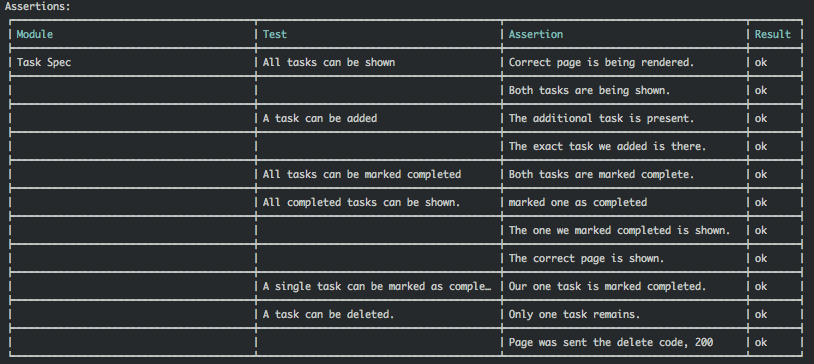
\includegraphics[width=\linewidth]{qunitrunner.png}
  \captionof{figure}{Each individual spec is further broken down into the assertions within it.}
\end{Figure}

An interesting feature that QUnit has is the ability to specify how many assertions are expected to run in the test. This is incredibly useful for callbacks. By setting an expected number of assertions, tests can no longer fail silently just because an assertion was never run. Silent failure can happen if the developer forgets to specify that a test is asynchronous or if there are synchronous callbacks. If a function in the test has a callback that runs the assertions, the test framework may finish executing the test and move on to the next test before ever running the assertions in the callback. If the QUnit test finishes and the assertion count is not what was specified, it will fail the test and let the developer know fewer assertions were called than expected.

QUnit tests are not grouped into suites by default and the syntax for grouping them leaves much to be desired. In order to group tests into ``modules'', as QUnit calls them, the developer writes code like the following:
\begin{lstlisting}
Qunit.module("Module A"); // All code following is grouped
test("Addition", function () {
  equal(2 + 2, 4, "Two + Two = Four");
  equal(3 + 5, 8, "Three + Five = Eight");
});
test("Subtraction", function () {
  equal(4 - 2, 2, "Four - Two = Two");
  equal(2 - 2, 0, "Two - Two = Zero");
});

// More tests....

QUnit.module("Module B");
// Tests now grouped under Module B
// ... Etc
\end{lstlisting}
It can be difficult to visually determine where one module starts and ends, resulting in additional time spent finding the right place to add a test.

QUnit's handling of asynchronous tests is similar to Mocha's except instead of adding a parameter to the \lstinline{it} function, the developer calls the \lstinline{asyncTest} function instead. Finally, the developer calls \lstinline{start()} when the asynchronous test is finished. Example:
\begin{lstlisting}
asyncTest("Async Test", function () {
  myAsyncCall(param1, param2, function () {
    // This callback expected to run when myAsyncCall finishes
    // Test ...
    // Test ...
    // ...
    start();
  });
});
\end{lstlisting}

QUnit provides another style of writing tests and grouping modules. QUnit's handling of asynchronous tests is nice because they are more explicitly stated for the casual read-through instead of an extra parameter or set of functions within the test itself.

\subsection{Intern}
Intern\cite{InternIO} is a hybrid unit testing and browser testing framework that aims to be an all-in-one testing framework. Intern has unit testing, browser testing, and code coverage information all built into the same tool. It is our intention to build a testing framework with all of these components, so finding a framework with all of them built-in was promising. Intern runs on its own server which give it access to the internals of the project, but caused problems when attempting to interact with a separate server running the Node.js application. We were unable to get the browser testing portion of Intern to work because of our inability to set up cross-server communication due to inexperience.

%-AMD
Intern uses Asynchronous Module Definition (AMD) form. This is merely a change in how modules are included in a piece of code, instead of separately requiring modules, the entire program is wrapped in a \lstinline{define([...])} block that passes modules as parameters to an overarching function. That will make more sense after an example:
\begin{lstlisting}
// Intern
define([ // Here's the AMD
    'intern!object',
    'intern/chai!assert',
    'app/hello'
], function (registerSuite, assert, hello) {
  // Test code here
});


// CommonJS, what Node.js uses 
var registerSuite = require('intern/object');
var assert = require('intern/chai/assert');
var hello = require('app/hello');

// Test code here


// Another way to write CommonJS so that it's not global scope, used frequently
(function () {
  var registerSuite = require('intern/object');
  var assert = require('intern/chai/assert');
  var hello = require('app/hello');

  // Test code here
} ());
\end{lstlisting}

Using either style you get access to the modules outlined. AMD form offers a tighter, more straightforward way to look at module loading in addition to being better supported and having fewer gotchas. \cite{AMDInfo} Intern offers support for CommonJS modules but strongly recommends switching to AMD styles for your project. We chose to keep our CommonJS format because that is what Node.JS uses, which is used by our evaluation applications.

%- TDD, BDD, Object methods
Intern uses Chai.js for assertion methods but has it built-in as opposed to Mocha in which the developer had to get it themselves. This gives the developer access to Expect, Assert, and Should testing methods. In addition to the various assertion styles, Intern offers three different testing interfaces: TDD, BDD, and Object. These testing interfaces effect how the general layout of test code looks. Here's a very quick example of the different layouts:
\begin{lstlisting}
// TDD
suite('TDD Suite', function () {
  test('test 1', function () {
    ...
  });
}

// BDD
describe('BDD Suite', function () {
  it('should be test 1', function () {
    ...
  });
}

// Object
registerSuite({
  name: 'Object Suite', 
  'test 1' : function () {
    ...
  },
  'test 2' : ...
)
\end{lstlisting}

The ability to mix assertion styles with testing interfaces provides a diverse way of writing tests. Some testing interfaces seems to fit better with certain assertion styles, but there's no restrictions on which can be used with which.

%- Integration with Selenium
Intern uses the WebDriver API to communicate with Selenium to drive the automated browser testing portion of Intern. Selenium and the WebDriver API will be discussed in more detail in the next section ``Browser and UI Testing''.

%- Distinction between non-functional and functional tests
Intern's unit-test versus browser test separation is termed, by Intern, nonfunctional versus functional testing. Nonfunctional tests are those that run without a browser while functional tests are WebDriver tests.

%- Code Coverage!
Intern includes configurable code coverage metrics on tests by default. Running unit tests gives the number of lines covered (ran) by the tests. Code coverage is provided by another JavaScript library, Istanbul, created by Krishnan Anantheswaran \cite{Istanbul}.

Intern offers a fully-featured framework for all testing needs but was difficult to configure for a Node.js server setup. If a developer had a more traditional web application setup with a separate server that served normal HTML pages, Intern would be a go-to framework for all testing needs.

\section{Browser and UI Testing}
Web applications, for the most part, require user input in order to be useful. The way the user interacts is through the outward facing web pages. Testing of a web application would be incomplete without testings the interactions and elements of these web pages. It's important that the inner workings are running the right code and producing the right answer, but it's almost just as important that the parameters get passed correctly and from the right places on the web pages. Also, it is important that navigation work as expected or a user will become frustrated and lose interest in the application.

What's important in browser testing is repeatability and being able to test on multiple browsers. Without the ability to automatically repeat tests, developers are left manually clicking through web pages every time anything changes. In addition, because there are so many different browsers and browser versions in the wild, it's important that the web pages run correctly (and predictably) on as many of them as possible.

\subsection{Selenium}
Selenium\cite{Selenium} is an automated browser driver. It is one of the only automated browser drivers; in all of our searching, we did not find a single other browser automation tool, all other frameworks were built on top of Selenium. A developer can write code that will cause Selenium to drive a browser's input and assert expectations. On its own Selenium has very minimal testing usage. It lacks a test reporting mechanism and only offers output in two forms: 1) No output at all, a browser window will open, input will be generated, and the window will close, or 2) the browser will exit with a cryptic error printed to the console. It is up to the developer to include print statements as to what is happening at any given time, what test is being run, and what the results are.

Generally, all browser testing tools will be using Selenium behind the scenes and doing the housekeeping automatically. This is the case for the web testing tools that will follow this description.

Selenium has support for running a number of different browsers. Out of the box it comes with support for Firefox but getting Chrome and Safari running takes minimal effort.

Having the ability to automatically run browser tests at any point takes a huge burden off of the web developer and allows for UI testing in addition to behind the scenes functionality testing. Whenever code is changed that may affect the UI flow or functionality, Selenium tests can be run without the need for developers to manually click all of the HTML elements and input information in the relevant places.

% This is talked about in the tutorial
% Selenium's Node incarnation is out-of-date and as such we had to change the Selenium package to use the latest version of Selenium that works with the latest version of browsers. This required us to edit some of the JavaScript files that ran Selenium from the console using Node. At the time of this writing, the Selenium node package was using Selenium 2.20 from over two years ago. The latest Selenium version is 2.40.

Selenium was written with maximum functionality and language flexibility in mind and therefore can be incredibly verbose.

The Selenium WebDriver has APIs for a variety of programming languages including: JavaScript, C, Java, and Python.

\subsection{Nightwatchjs}
Nightwatch\cite{NightwatchJS} is a JavaScript testing library that wraps Selenium in an effort to make browser testing more concise and straightforward. Nightwatch uses Node.js' assertion library paired with Selenium's WebDriver to both run browser automation and also report test results.

Tests are written as a long chain of function calls that produce an easy-to-read series of browser events. For example, the following code segment opens a browser, goes to Google.com, makes some assertions, writes ``nightwatch'' in the search box, clicks the search button, and then makes a few more assertions:
\begin{lstlisting}
module.exports = {
  "Demo test Google" : function (client) {
    client
      .url("http://www.google.com")
      .waitForElementVisible("body", 1000)
      .assert.title("Google")
      .assert.visible("input[type=text]")
      .setValue("input[type=text]", "nightwatch")
      .waitForElementVisible("button[name=btnG]", 1000)
      .click("button[name=btnG]")
      .pause(1000)
      .assert.containsText("#main", "The Night Watch")
      .end();
  }
};
\end{lstlisting}
As one can see, just reading the code line by line paints a picture of exactly what is happening and what is being checked for. 

The same code in normal Selenium is quite a bit more verbose:
\begin{lstlisting}
var assert = require('chai').assert,
    test = require('selenium-webdriver/testing'),
    webdriver = require('selenium-webdriver');

test.describe('Google Search', function() {
  test.it('should work', function() {
    var driver = new webdriver.Builder().
        withCapabilities(webdriver.Capabilities.chrome()).
        build();

    driver.get('http://www.google.com');
    driver.findElement(webdriver.By.name('q')).sendKeys('nightwatch');
    driver.findElement(webdriver.By.name('btnG')).click();

    driver.sleep(1000);
    driver.findElement(webdriver.By.id('main')).getText().then(function (text) {
        assert.isTrue(text.indexOf("The Night Watch") !== -1);
        driver.quit();
    });
  });
});
\end{lstlisting}

In addition to being more verbose, we've had to add an assertion library and this code has to be run using Node.js and the Mocha module instead of using the Selenium command. By default, Selenium does not come with its own assertion library. We chose Mocha with Chai.js because we were most familiar with it.

Nightwatch is a Node.js module, and as such can easily installed and run via npm and the commandline.

Though a small feature, Nightwatch has the ability to either assert or verify tests. The difference is that assertions will stop execution while verifications will merely log the failure and continue on. Verification can be useful if the developer wants to get an update on how many things are currently failing as opposed to having the entire test stop executing immediately after a single failure.

Nightwatch, as of this writing, has the ability to open Firefox, Chrome, and Internet Explorer. As of February 2014, Chrome is used by 46.69\% of internet users, Internet Explorer is used by 24.39\% and Firefox is used by 20.78\%.\cite{BrowserStats} Together that accounts for 91.86\% of all internet users.

\subsection{Headless Browsers}
In an attempt to speed up UI testing, which is notoriously slow, there have been efforts to create ``headless'' browsers which behave like normal browsers except that there's no display element. They emulate the DOM and skip the display phase. We opted to stick with visual browsers due to time constraints and the added complexity of running headless browsers.

Nonetheless, we still looked at two options that we will outline briefly below for other developers' reference. The two options outlined below by no means cover all of the headless browser options, they are simply the two that we saw most often discussed by the other testing tools.

\subsubsection{PhantomJS}
PhantomJS\cite{PhantomJS} came up repeatedly in our searches for testing frameworks as an option for headless browsing; it is the reason we had the idea to look into headless browsers. PhantomJS is a headless browser written using WebKit, which is what most of the web is based on. This means that running PhantomJS is nearly indistinguishable from a normal browser to any testing code.

There are, however, a couple problems with PhantomJS. It is generally fairly verbose when it comes to writing the scripts that run your commands. It is also not a testing tool, it is a headless WebKit. The distinction here is that PhantomJS does not have any assert functionality built-in and thus requires the developer to find and use their own assertion library.

The difference between PhantomJS and ZombieJS, which I talk about in the next section, is akin to the difference between Selenium and Nightwatch. PhantomJS is heavier duty and requires an additional set of testing tools whereas ZombieJS is lightweight and has assertions built-in.

\subsubsection{ZombieJS}
ZombieJS\cite{ZombieJS} is the other headless browser that we saw when searching for browser testing tools. ZombieJS is not a WebKit implementation but rather a simple DOM emulator. This means that certain tests may not be as accurate as they could be with PhantomJS.

Where ZombieJS shines is in its simplicity and brevity. Much like Nightwatch, calls are chained together to create a flow of calls that generally end with assertions.

\begin{lstlisting}
// Zombie.js website's example code
var Browser = require("zombie");
var assert = require("assert");

// Load the page from localhost
browser = new Browser()
browser.visit("http://localhost:3000/", function () {

  // Fill email, password and submit form
  browser.
    fill("email", "zombie@underworld.dead").
    fill("password", "eat-the-living").
    pressButton("Sign Me Up!", function() {

      // Form submitted, new page loaded.
      assert.ok(browser.success);
      assert.equal(browser.text("title"), "Welcome To Brains Depot");
    });
});
\end{lstlisting}

Developers like ZombieJS syntax so much that there exists a wrapper that uses ZombieJS's API around PhantomJS. \cite{ZombiePhantom}

ZombieJS offers a lightweight solution to headless browser testing, but does not have the same depth of features as PhantomJS or the same assurances that your tests do exactly what they would do in a browser with a head.

\section{Continuous Integration Frameworks}
Continuous Integration frameworks attempt to make development easier by running specified actions, usually tests, after a change to the project. This change can be simply saving a modified file, or, more usually, an action like pushing a change to a repository.

Continuous Integration frameworks, therefore, need to be flexible in the type of project they support, customizable in their chosen environments to support differing projects, and have a simple way to connect to repositories or file systems.

\subsection{Jenkins}
Jenkins\cite{Jenkins} is an offline Continuous Integration tool, the only offline tool that we found with active developement and support. It was created by developers of a previous tool called Hudson when a dispute with Oracle led them to fork the Hudson project and rename it Jenkins. As of February 2014, the Jenkins organization has over 1,100 public repositories and 570 members. \cite{JenkinsGitHub} Jenkins has, according to their website, two main focuses: (1) building and testing software continuously and (2) monitoring executions of externally-run jobs. The first focus is the general goal for any CI framework. The second focus is of note and will be discussed after the initial evaluation. 

Jenkins is a series of web pages that are set up to run on a given server. This is what it looks like:
\begin{Figure}
  \centering
  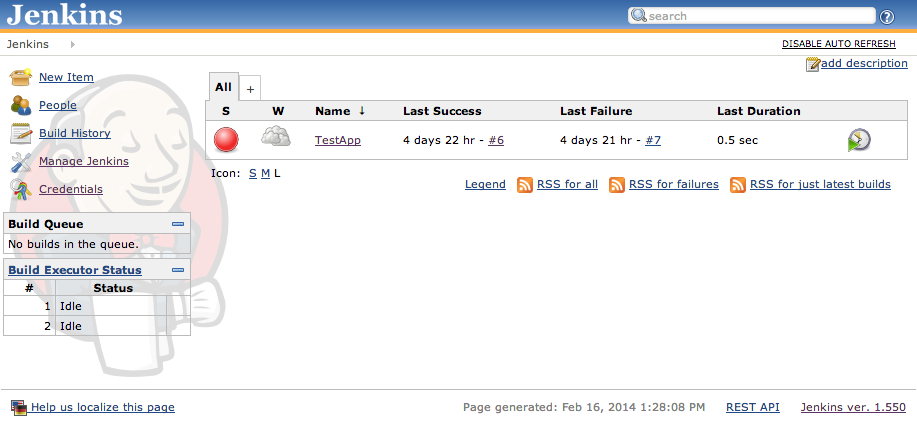
\includegraphics[width=0.95\linewidth]{jenkins.png}

\end{Figure}
Most companies give Jenkins a sub-domain on their web pages.

Jenkins comes bare-boned but is highly customizable and has a wide array of plugins. The plugins available integrate Jenkins with various services, integrate Jenkins with source control systems, and even just change the look of the Jenkins page or how it behaves. As an example, Jenkins can integrate with GitHub to run builds and tests when changes are pushed to a branch.

Because Jenkins comes bare and runs on the system of the developer's choosing, it can run any project that is set up. The downside is that there is no support out-of-the-box unless the system already has the necessary compilers, interpreters, applications, and/or libraries installed.

One of the exceptional strengths of Jenkins is that the developer is only limited by the hardware of the machine running Jenkins. Jenkins can run an ``unlimited'' number of builds, tests, and processes with the only limiting factor the hardware that it is running on.

The other use for a tool like Jenkins is the ability to start services like cron jobs or similarly long-running tools and status monitors and then collect the output for them and allow the developer to check on them at any time.

Jenkins is an exceptionally strong tool for CI, but requires immense overhead in setting up the environment to run a project in. However, once the server has the necessary applications and libraries, the developer can run builds and tests. Jenkins is 100\% free and can connect with public and private repositories alike.

\subsection{Travis}
Travis\cite{Travis} is an online continuous integration framework with 29 active developers working to improve it and 64 repositories that support it at the time of this writing. Unlike Jenkins, Travis is all online and includes a dashboard from which the developer can monitor builds and processes. Travis has a free version which is fully-featured but requires the project to be open-source and a paid version which gives the developer more processing power and access to private repositories.

Travis comes with internal support for eleven different languages including Node.JS, Ruby, Java, and Python. Travis has incredibly thorough documentation and a wealth of built-in services to work with projects if needed. Theses services include databases, notifications, deployment options, and GUI/Headless browsers. Travis supports all of the most popular databases: MySql, PostgreSql, MongoDB, CouchDB, and a myriad of others. It offers a number of notification options ranging from Email to IRC to HipChat (a chat service from Atlassian). Travis also offers deployment to just about every sort of provider there is, from Heroku to AWS S3 to RubyGems and also provides the ability to create custom web hooks to deploy to a provider not supported natively.

If at any point the project requires something that Travis does not support natively, Travis gives the permissions necessary to install any sort of libraries or services that can be installed with apt-get on an Ubuntu machine.

Travis requires that projects be hosted on GitHub, but by doing so the setup is incredibly easy. The developer signs into Travis using GitHub credentials and Travis pulls up all of the developer's repositories automatically. 

Getting a project running with Travis is fairly easy; just create a yml file in the repository with certain lines pertaining to the language, needed services, commands to run, etc. We were able to set up everything we needed in six simple lines.

In order to get access to private repositories, Travis offers several pricing plans, the cheapest of which is \$129 \cite{TravisPricing} for their ``Startup'' plan. That's a bit steep, but it does offer unlimited private repositories, unlimited collaborators, and two concurrent jobs. 

From what we gathered, Travis appears to be targeted at companies, not individual developers. Travis requires developers to host their projects on GitHub and only supports one process running at a time. However, Travis is incredibly easy to set up, does not require it's own server, comes with impressive built-in features, and works wonderfully with open-source repositories on GitHub.

\subsection{Semaphore}
Semaphore\cite{Semaphore} is an online CI framework that connects to GitHub to bring in projects. Semaphore is made by RenderedText, a software consulting team. Semaphore connects with public and private repositories but requires a subscription after 30 days no matter which repositories are used.

Semaphore was originally designed for only Ruby applications but in January of 2014 they announced official support for Node.js and JavaScript and as of February 26th they now offer official support for Clojure projects.\cite{SemaphoreBlog} These types of projects require no setup or files in the repository, Semaphore automatically detects project type and auto-fills build steps. Their ``supported stack'' page also lists C/C++, Java, Perl, and Python, but those must be configured manually. 

Semaphore supports most databases and has a number of testing frameworks built-in. Once again any missing libraries or dependencies can be installed using apt-get. It would appear that deployment support is only available for Ruby projects.

Semaphore's pricing scheme is different than Travis' as it focuses on an individual, not a company. Their lowest cost subscription is one project (public or private) for \$14 per month. They offer more subscriptions with the ability to have more projects and concurrent processes in higher tiers.

Semaphore is still ruby-centric and requires a subscription. As our goal is to find a framework that is free for open-source projects, Semaphore was out automatically. It is included here because it's well-known and fairly established, especially in the ruby community.

\subsection{MagnumCI}
MagnumCI\cite{MagnumCI} is another online CI framework. MagnumCI has every feature available for free, however, it's still in public beta and although prices haven't been released, the team making MagnumCI has already stated that there will be price tiers. It is not unreasonable, though, to believe that MagnumCI will be free for open-source projects.

MagnumCI offers support for Ruby, PHP, Node.JS, and Go. MagnumCI, much like Semaphore, will attempt to auto-detect commands that it should run based on the project structure and language. All settings are able to be overridden in a yml file.

MagnumCI has all the popular databases built-in, many of which run automatically on startup. MagnumCI also has two headless browser frameworks built in for running any browser testing that needs to be done. The developer can, again, use apt-get to install missing packages. MagnumCI does not, at current, provide automatic deployment options given a successful build.

Where MagnumCI shines is in support of different repositories. MagnumCI offers support for pulling from GitHub, BitBucket, GitLab, and a few others. It does require a bit more setup to get repositories connected, but what it comes down to is a couple lines of copied and pasted text within the repositories' settings.

Right now MagnumCI offers impressive features, private repositories, and extensive repository sources, all for free. It is hard to say that MagnumCI is the best because those features may end up costing money soon after this paper is completed. It is included in this review because it seems to be an up and comer that could prove quite strong.

\subsection{Drone.io}
Drone.io\cite{DroneIO} is an impressive online CI framework that offers substantial language support, is free for open-source projects, and offers the most reasonable pricing scheme for private repositories.

Drone.io supports eleven languages including: C++, Dart, Go, Haskell, Java, Node.JS, Ruby, and others. Setup requires the developer to specify language, as opposed to the automatic tools provided by the previous two CI frameworks, but will auto-generate build commands.

Drone.io offers support for an impressive number of databases, has a variety of deployment options, and is entirely configurable from the online dashboard. It also offers the most browsers and headless browsers for use with web page testing tools such as Selenium and PhantomJS.

Drone.io is able to connect to GitHub, BitBucket, and Google Code repositories to get projects automatically. Setup is simple, select the source of the repository (GitHub, BitBucket, or Google Code), select the repository from the list it gives once it connects, select the language of the repository, edit the default build script, and the project is ready to go.

Drone.io offers unlimited free open-source repositories. The next step up offers 5 private repositories for \$25 per month and for \$50 per month, unlimited private repositories. They also offer higher tier plans that allow for concurrently running builds.

Drone.io is a strong contender because of its language support, deployment options, and ease of setup. Where it lacks is in its notification options. The only notification option at present is email while other CI frameworks offer a number of other notification options for various messaging services.

\subsection{Manual Continuous Integration}
Most of what these CI frameworks accomplish can be done by hand with enough script writing. Continuous Integration tools are notified of updates by scripts that run after a commit is pushed. With the Continuous Integration scripts above, the post commit scripts are written without the knowledge of the developer. There is, however, no reason that a developer cannot hook into those scripts themselves.

Manual CI is incredibly similar to Jenkins in that its only limitations are the libraries and hardware that it's run on.

There are a few differences between Jenkins and Manual CI, the biggest being that Jenkins has a GUI. This GUI is used to configure the project while manual CI requires script and text editing. 

Another big difference between Manual CI and all of the other CI frameworks is that the non-manual frameworks store information regarding the status of builds, the success and failure of builds, which files changed in each commit, and a lot of other information that can be quickly viewed. It is possible to store this information manually, but it would require considerable effort to make it as easy to use as the other CI frameworks.

Finally, manual CI uses a developer's system, rendering it unusable to the developer, particularly during the UI testing phase. The developer must accept a productivity hit every time they commit to their repository.

\section{Miscellaneous Frameworks}
In addition to the Unit Testing, Continuous Integration, and Browser Testing frameworks outlined above, we came across a number of incredibly helpful frameworks that did not quite fit into any of the above categories.

\subsection{Sauce Labs}
Sauce Labs\cite{SauceLabs} is an online service that gives you access to a variety of browsers and browser options. They outline the options available to the developer as follows: Selenium, JavaScript, Mobile, Manual. Sauce Labs will start up a Selenium server and run the developer's Selenium tests, they can run unit tests using their JavaScript service, they allow access to a variety of mobile device browsers and resolution, and they offer the ability to manually look at a web application in different browser configurations.

Every CI framework we looked at had built-in configurations for Sauce Labs so that one of the CI steps could be running your tests on Sauce Labs.

Sauce Labs is an incredibly helpful tool for making sure a web application behaves as expected on a wide spectrum of devices and configurations and saves the developer the hassle of acquiring multiple devices, operating systems, and browsers.

\subsection{Istanbul}
As already mentioned briefly, Istanbul\cite{Istanbul} is a tool used for code coverage metrics. It was built into Intern.io but getting it running with other frameworks is easy as well.

Getting Istanbul to output code coverage is as easy as installing it and then calling the \lstinline{istanbul} function from the commandline with your test executable.
For example: \lstinline{istanbul cover mocha -- . -R spec} will run the mocha tests in the current directory and output coverage statistics. To break that down a little further:

\lstinline{istanbul cover} tells istanbul to run coverage on the tests.

\lstinline{mocha --} specifies that the executable to be run is mocha and that the developer is done giving commandline arguments to istanbul, that's the \lstinline{--}

Finally, \lstinline{. -R spec} is just the flags for the mocha command to run the appropriate test suites.

Istanbul offers an incredibly easy way to get code-coverage on your tests and is painless to get working right away.

\subsection{Grunt.js}
Grunt.js\cite{GruntJS} is a task-runner for JavaScript. What Grunt does is automate routine tasks like linting, testing, copying files, and updating modules. The developer writes Grunt scripts that outline the necessary tasks and then can run them on the commandline with the \lstinline{grunt} command.

Grunt is widely supported and has all kinds of built-in or installable plugins that make writing common tasks nearly trivial. As an example, a few built-in grunt tasks that we use include: \lstinline{jshint} for linting, \lstinline{uglify} for code minimization, and \lstinline{watch} for automatically re-running tests when certain files change. Each of those plugins requires very little configuration and they're ready to be used.

Of particular interest is that last feature, \lstinline{watch}. We use grunt's \lstinline{watch} capability to run tests constantly. This feature gives immediate feedback to the developer when they change existing code or write new code after having written a test for it. As long as all the tests are passing, the developer has a good idea that the changes made are regression-tested as well as freshly tested and are ready for publishing or integration.

\subsection{Node Inspector}
Node Inspector\cite{NodeInspector} is a GitHub project for debugging Node.js server-side code. The inspector runs in the browser and is started by running \lstinline{node-debug} instead of \lstinline{node} when starting the application. Simple as that. Then you can set breakpoints using the normal browser developer tools.

Currently Node Inspector only runs on Chrome and Opera but since those browsers are available on all OSes, it shouldn't be a problem for developers to use.

\section{Framework Decision Matrices}
In an effort to further expedite the selection of tools, the following decision matrices can be quickly referenced by new developers to decide on which tools are right for them.

\FloatBarrier
\begin{table}[ht]
\resizebox{\textwidth}{!}{%
\begin{tabular}{|c|c|c|c|c|c|c|}
\hline
Framework & Assertion Styles  & Test Interfaces & Reporters & AMD & Active Development*   \\ \hline
Jasmine   &                   &                 &           &     & X                     \\ \hline
Mocha     & X**               & X               & X         &     & X                     \\ \hline
Qunit     &                   &                 &           &     & X                     \\ \hline
Intern    & X                 & X               & X         & X   & X                     \\ \hline
\end{tabular}
}
\captionof{table}{Decision Matrix for Unit Testing Frameworks}
\end{table}
\FloatBarrier
\footnotesize

* Active Development is defined as any commit within the last month.

** Mocha requires a separate assertion, which leaves the options for assertion styles entirely up to the developer.

\normalsize
\FloatBarrier
\begin{table}[ht]
\resizebox{\textwidth}{!}{%
\begin{tabular}{|c|c|c|c|c|c|c|}
\hline
Framework & GitHub & Other Repos & Multi-Language & Active Development** & GUI Configuration \\ \hline
Jenkins   & X*     & X*          & X*             & X                    & X                 \\ \hline
Travis    & X      &             & X              &                      &                   \\ \hline
Semaphore & X      &             & X              & X                    & X                 \\ \hline
MagnumCI  & X      & X           & X              & X                    & X                 \\ \hline
Drone.io  & X      & X           & X              & X                    & X                 \\ \hline
Manual    &        & X           & X              & X                    &                   \\ \hline
\end{tabular}
}
\captionof{table}{Decision Matrix for Continuous Integration Frameworks}
\end{table}
\FloatBarrier
\footnotesize

* Jenkins has the ability to do all of the things listed with enough time devoted to setup.

** Active Development is defined as any commit within the last month.

\normalsize
%%%%%%%%%%%%%%%%%%%%%%
%%% Implementation 
%%%   Why we chose the tools we chose
%%%   Scripts written to help out 
%%%%%%%%%%%%%%%%%%%%%%
\chapter{Framework Selection}
In this chapter, we will outline our final choices for frameworks and why we chose them.

\section{Chosen Tools}
After evaluating a number of different combinations and tools, we came to the following setup:
\begin{itemize}
  \item Unit Testing: Mocha with Chai.js
  \item Continuous Integration: MagnumCI
  \item Browser Testing: Nightwatch
  \item Misc:
    \begin{itemize}
      \item Coverage: Istanbul
      \item Task Runner: Grunt
      \item Package Manager: NPM (sort of a given when working with Node.js)
    \end{itemize}
\end{itemize}

\subsection{Mocha with Chai.js}
Our choice of using Mocha with Chai.js was made because Mocha offers the flexibility of choosing one's own assertion library and testing interface while still having a default structure that all developers can read and code.

Mocha was chosen over Jasmine because of Mocha's additional flexibility and the way that Mocha handles asynchronous tests.

Mocha was chosen over QUnit because of the ability to structurally portray test suites. Although QUnit output a more thorough test summary, the ability to scan code more efficiently was of greater importance to us.

The final decision came down to Mocha versus Intern. Mocha was eventually chosen over Intern because of the ability to choose an assertion library and because of the issues we had with Intern. Both frameworks offer impressive flexibility regarding the way in which tests can be structured and written. Mocha ended up allowing for a bit more flexibility and caused no problems for us. Perhaps with more time and patience we would have chosen Intern, but Mocha served our needs well.

\subsection{MagnumCI}
MagnumCI has all of the features that a developer might need for free. We are still confident that the features needed by an open-source developer will continue to be free after MagnumCI ends its open-beta period.

Given enough resources and time, Jenkins will offer more support and functionality than the rest of the CI frameworks. However, there's something to be said for ease of setup and total time to first use of a tool. MagnumCI offered quick initialization through web pages and automatic repository connections that allow users to quickly configure and run the CI framework.

MagnumCI was chosen over Travis because our evaluation application was not on GitHub. Travis is still an incredible CI framework that has some of the best documentation among the CI frameworks. If a developer has their project on GitHub, we would recommend Travis over MagnumCI.

Semaphore's lack of support for JavaScript and Node.js projects as well as the GitHub requirement kept us from choosing it.

Drone.io, while offering a number of repository location options, did not offer the ability for a repository to be hosted at a custom location.

MagnumCI was chosen over manual CI for much the same reasons as it was chosen over Jenkins. Manual CI requires an extraordinary effort on the part of the developer if they wish to have all of the features and history of the other CI frameworks.

Overall, the CI frameworks were all impressive and usable. The main driving factor behind our decision was that our application used a custom repository and that at the time of this writing our application is closed-source. We have every intention of opening it to the public as soon as we get a version that is more polished.

\subsection{Nightwatch}
The choice for Nightwatch was an easy one. First and foremost there were not many options and the options we did have sorted themselves out.

Nightwatch, being a wrapper around Selenium already, was chosen over Selenium because of its concise way to express tests. We have yet to come across any situation that is not covered with Nightwatch as the developer of Nightwatch has seemed to implement nearly all WebDriver calls, even if some are undocumented.

Nightwatch was chosen over Intern's UI testing tool because of the issue with Intern running its own server. If Intern did not impose its own server for what it calls ``functional'' testing, we would probably have gone with Intern for both Unit and UI testing. Intern is a strong choice for an all-in-one testing tool.

\subsection{Miscellaneous Tools}
Generally the miscellaneous tools were chosen because they were already integrated into our project or were the obvious choices for other reasons.

Istanbul was chosen because of the ease of set up in getting it running using our existing toolset and project. There are other code coverage tools but Istanbul required so little setup that we chose to not look further.

Grunt was already a part of the evaluation application prior to the testing effort we set out on. With a bit of looking into Grunt, it was an obvious choice to keep it as our new functionality was easily integrated into the existing grunt scripts.

NPM is the go-to choice for acquiring modules for Node.js applications.

%%%%%%%%%%%%%%%%%%%%%%%%%
%%% Product 
%%% User Manual
%%%   Tools (programs, IDEs, scripts)
%%%   Setup instructions
%%%   Usage
%%%%%%%%%%%%%%%%%%%%%%%%%
\chapter{Testing and Development Workflow}
In this section we will mention our development setup, discuss how to set up the chosen tools, and outline our recommended workflow using the tools. It is our hope that after finishing this section, the reader will be able to install and run the chosen tools and have a good grasp of what the next steps are for their particular project.

\section{Our Implementation Configuration}
The following are the specs of the laptop that we used for the entirely of this research and implementation:
\begin{itemize}
  \item Model: 15-inch Macbook Pro, Late 2008
  \item OS: OS X 10.9.2, Mavericks
  % \item Processor: 2.53 GHz Intel Core 2 Duo
  % \item Memory: 4 GB 1067 MHz DDR3
  % \item Graphics: NVIDIA GeForce 9400M 256 MB
\end{itemize}
The point of listing the laptop specs is to show that our research and workflow was completed on an average, everyday laptop and does not require any kind of special hardware or software configurations. In addition, our setup instructions will be OS X based, but nearly all commands will work the same on another UNIX-based system.

To carry out the development we used a combination of the OS X terminal, Sublime Text, and Netbeans. The terminal was used mainly for starting Node services, testing tools, Grunt scripts, and for updating modules. Sublime Text was used to write the unit tests and the UI tests. Netbeans was used to quickly navigate through the code as it had already been set up as a series of Netbeans projects.

\section{Tool Setup}
Getting the tools up and running is a fairly simple task. It involves installing modules with NPM, writing or copying a few configuration scripts, and then using the terminal commands for running the tests.

We decided to install the node modules globally, but it's not a requirement. Tests can be executed using locally installed node modules. Instead of using the command by itself, the developer would just need to supply the full path to the executable, which is generally \lstinline{./node_modules/MODULE_NAME/bin/MODULE_NAME} \space instead of \lstinline{MODULE_NAME}. For example, a globally installed Mocha executable can be run with \lstinline{mocha ...} while a locally installed Mocha module is run with \lstinline{./node_modules/mocha/bin/mocha ...} \space .

Following the setup instructions will be a more thorough Gruntfile that can serve as a template and starting point for developers. The Gruntfile will have tasks that will run the Unit Testing and the UI Testing.

\subsection{Setting up Mocha}
To install Mocha, type into the terminal: \lstinline{npm install -g mocha}. The \lstinline{-g} means to install the module globally. The developer need simply skip the \lstinline{-g} in all of the following install commands if they want the modules installed locally.

Next, to install Chai, type into the terminal: \lstinline{npm install -g chai}.

To get Chai running with Mocha, just \lstinline{require(...)} the appropriate chai assertion method in a test file and start writing. For example, to get the Assert library: \lstinline{var assert = require('chai').assert;}

The tests can be put in any folder, but something to keep in mind is that the tests will reference the source code. The further away from the source code the tests are, the longer the paths to the source code in the test files.

For reference here's what a simple test file might look like:
\begin{lstlisting}
// repo/src/tests/myTestFile.js

var assert = require('chai').assert;

describe("My Test Suite", function () {
  var myModule = require('../my_module.js');

  it("should run my function", function () {
    var result = myModule.myFunction();
    var expected_result = 10;

    assert.equal(result, expected_result);
  });
});
\end{lstlisting}

After the tests have been written, the developer can run them using the \lstinline{mocha} command. There are a number of command-line arguments available to the mocha command which are well documented and which we won't talk about here. We will talk about the one that we used consistently, that being \lstinline{-R}. The \lstinline{-R} argument allows the developer to specify how the test results will be printed and formatted. Mocha offers seventeen different reporters with more reporters available online and the ability to create custom reporters. We chose the \lstinline{spec} reporter because it outlined each individual suite and test case. Other reporters generally provide less information such as the \lstinline{progress} reporter which just shows a progress bar. All together, our mocha test command was \lstinline{mocha -R spec .}, the final \lstinline{.} being the directory where the tests are located.

\subsection{Setting up MagnumCI}
Setting up MagnumCI is all done online. Visit ``magnum-ci.com'', create an account, sign in, click on ``Add a New Project''.

Here is the new project page:
\begin{Figure}
  \centering
  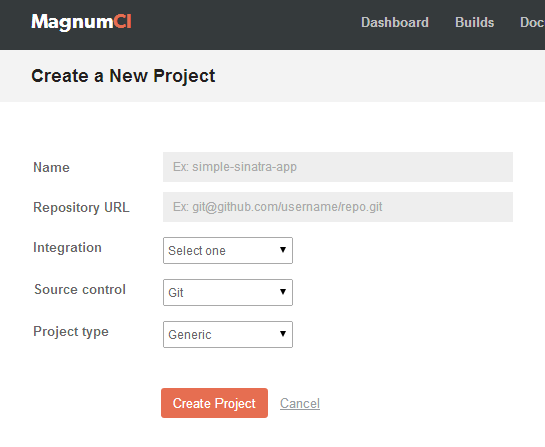
\includegraphics[width=0.75\linewidth]{magnumCI_new_project.png}
\end{Figure}

Fill out the fields with the appropriate values for a given project and click ``Create Project''. Depending on what the setup is for your project, you'll see slightly varying web pages after you create your project. One thing in common, though, is the button at the bottom of the steps list that says ``Customize Build''. After following the instructions, click ``Customize Build'':
\begin{Figure}
  \centering
  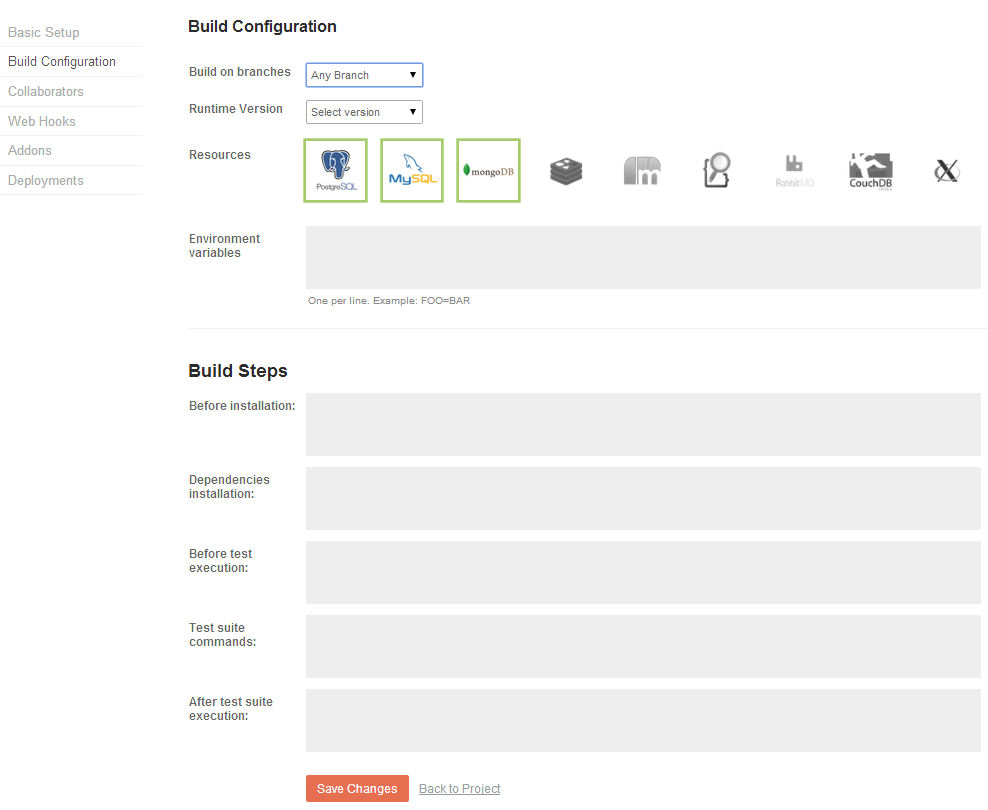
\includegraphics[width=0.75\linewidth]{magnumCI_customize_build.png}
\end{Figure}

There are a number of configuration options and panes that can be accessed on the left side. Our focus was making sure the ``Build Configuration'' tab was properly set up. This involved selecting the correct branch, the correct Node.js runtime version, the correct database from the ``Resources'' area, and adding the appropriate commands in the build steps. In our case we wanted ``mongoDB'' and ``Xvfb'' for UI testing, and then \lstinline{npm install -g} in the ``Dependencies Installation'' to make sure our modules are available when we need them. Finally, we run Nightwatch using \lstinline{nightwatch -c nightwatch.json} (the nightwatch flags will be outlined in the next section) in the ``Test suite commands'' box. All of that makes our build configuration page look like this:
\begin{Figure}
  \centering
  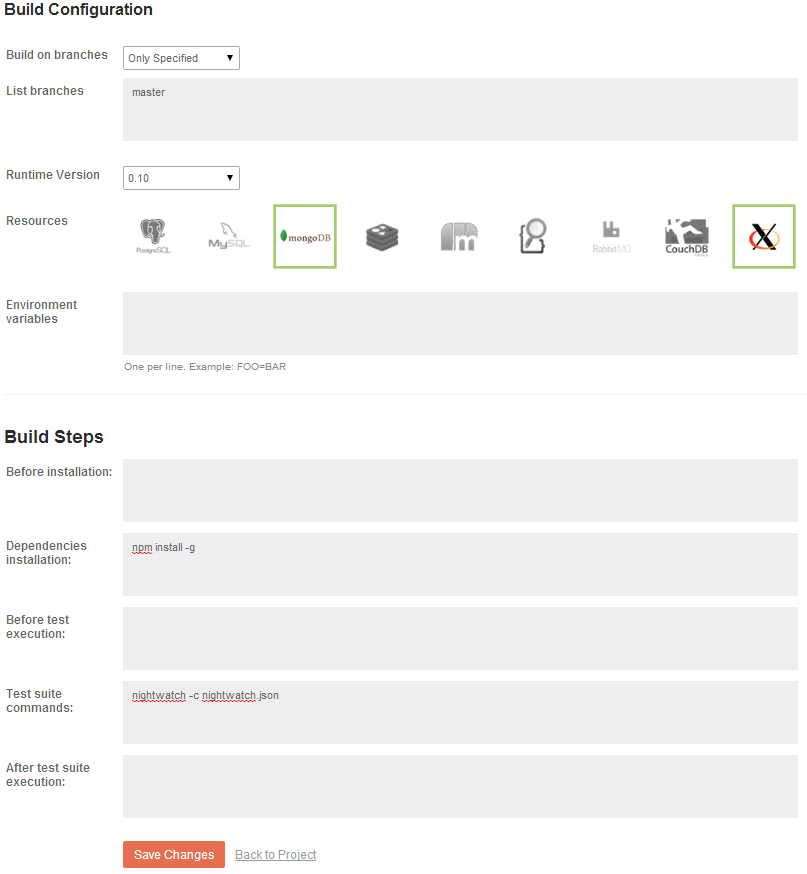
\includegraphics[width=0.75\linewidth]{magnumCI_customize_build_filled.png}
\end{Figure}

After that setup, the project is ready to go. Anytime a commit is pushed from then on, MagnumCI will run and notify the developer of successful and unsuccessful builds.

\subsection{Setting up Nightwatch}
Installing Nightwatch consists of just installing another npm module. \lstinline{npm install -g nightwatch}. In addition to Nightwatch, the developer needs Selenium. The easiest way is to just download the ``selenium-server-standalone'' jar straight from the Google repository here: ``http://selenium-release.storage.googleapis.com/index.html''. Our tests ran using ``selenium-server-standalone-2.40.0'' but any version 2.40+ should work. Once the developer has the JAR and places it in a location they will remember, generally along with other similar executables in a bin or library directory, Nightwatch is ready to be configured and run. Nightwatch configuration happens in a json file that is pointed to when the developer executes Nightwatch. 

The configuration file has plenty of options to get Nightwatch to do exactly what the developer wants, some of the more important ones include the \lstinline{selenium} object that holds information about where the executable is located and what ports to run on, the \lstinline{src_folders} attribute to specify a source directory, and the \lstinline{test_settings} object that contains configurations for default web pages, differing environments, and some desired capabilities. 

To run Nightwatch, navigate to the project folder and run \lstinline{nightwatch -c path_to_nightwatch_config}. This will use the \lstinline{src_folders} attribute to determine where to look for the tests, start the Selenium server, and run the tests. When debugging certain functions of even test cases, tests can be isolated with the \lstinline{-t} flag: \lstinline{nightwatch -c nightwatch.json -t folder1/test1.js}. Nightwatch offers a number of other command-line arguments that are discussed in their developer guide. \cite{NightwatchJS}

\subsection{Setting up Istanbul}
As mentioned in the Istanbul section, getting it running is simple. Install Istanbul with npm: \lstinline{npm install -g istanbul} and then run the istanbul command along with any others needed. In our case, we ran \lstinline{istanbul cover mocha -- . -R spec} to run Istanbul on our Mocha unit tests. For a more detailed view of possible commands and arguments, the developer can check out the Istanbul page. \cite{Istanbul}

\subsection{Setting up Grunt}
Getting Grunt set up just the way the developer wants it is the most involved, but there are a myriad of examples and sample scripts to help them through. Installation is the same as we've seen before, \lstinline{npm install -g grunt-cli}. After installation the developer will need to create a ``Gruntfile'' which is just a JavaScript file named ``Gruntfile.js''. Inside the Gruntfile are all of the command names and procedures that the developer wants. As the documentation outlines: ``A Gruntfile is comprised of the following parts: 1) The \"wrapper\" function 2) Project and task configuration 3) Loading Grunt plugins and tasks 4) Custom tasks''. \cite{GruntJS}

Here is an example Gruntfile:
\begin{lstlisting}
// 1) Wrapper Function
module.exports = function(grunt) {

  // 2) Project configuration.
  grunt.initConfig({
    pkg: grunt.file.readJSON('package.json'),
    uglify: {
      options: {
        banner: '/*! <%= pkg.name %> <%= grunt.template.today("yyyy-mm-dd") %> */\n'
      },
      build: {
        src: 'src/<%= pkg.name %>.js',
        dest: 'build/<%= pkg.name %>.min.js'
      }
    }
  });

  // 3) Load the plugin that provides the "uglify" task.
  grunt.loadNpmTasks('grunt-contrib-uglify');

  // 4) Default task(s).
  grunt.registerTask('default', ['uglify']);
};
\end{lstlisting}

In this simple Gruntfile, all that is happening is some configuration and the creation of an ``uglify'' task that will obscure the code when run.

A more complicated Gruntfile simply consists of more tasks. Taken one at a time, it's easy to pick apart a Gruntfile. Task names can refer to one or more commands, so the command \lstinline{grunt testMyStuff} may run one command, or may run five commands. The task names are the ones that are used as the first parameter of the \lstinline{registerTask} call.

\section{Suggested Workflow}
In addition to just a list of tools and installation instructions, we'd like to propose a way to use those tools that is efficient and nearly autonomous. Our goal is to bring testing tools into use with as little resistance as possible. With a bit of effort at the outset, testing can become a crucial and enjoyable part of development.

What we recommend is a unit test suite that runs on save. While this may seem excessive, it provides invaluable, instant feedback for regression assurance and new functionality. The way to set this up with the above tools is have a grunt task that watches for changes in certain files and runs a script when the files change. Here's what our Grunt task looks like:
\begin{lstlisting}
module.exports = function(grunt)
{
  grunt.initconfig({
    watch: {
      test: {
          options: {
              spawn: false
          },
          files: ['**/*.js'],
          tasks: ['mochaTest']
      }
    },
    mochaTest: {
      test: {
          options: {
              reporter: 'spec',
              clearRequireCache: true
          },
          src: ['../../../../NetBeans/PolyXpressAuthor/test/unit/functional/*.js']
      }
    }
  });

  // Specify the test directory for Watch to keep track of
  var defaultTestSrc = grunt.config('mochaTest.test.src');
  grunt.event.on('watch', function(action, filepath) {
      grunt.config('mochaTest.test.src', defaultTestSrc);
      if (filepath.match('test/functional')) {
        grunt.config('mochaTest.test.src', filepath);
      }
  });

  grunt.loadNpmTasks('grunt-contrib-watch');
  grunt.loadNpmTasks('grunt-mocha-test');

  // Register the mocha test task
  grunt.registerTask('test', ['mochaTest', 'watch:test']);
}
\end{lstlisting}

Our gruntfile is more complex than just that, but those are the parts that make the test-on-save functionality work. As we said earlier, Grunt has a lot of plugins that are available. We use one here to make our lives easier, \lstinline{grunt-mocha-test}. It is installed, once again, through npm and gives us access to the now-built-in task \lstinline{mochaTest}. The run-on-save functionality comes from the \lstinline{watch} task which has \lstinline{mochaTest} in its \lstinline{tasks} array.

Once that setup is done, the developer just runs \lstinline{grunt --force test} once which will execute the tests and then watch for changes and continue testing on save. The \lstinline{--force} flag is used so that the grunt task continues after ``failure'' which would occur if any tests did not pass.

For running the browser tests, we recommend using the CI tool. Most CI setups have Xvfb (a windowless X11 process) and some even have Firefox pre-installed. Nightwatch requires both to be installed. If Firefox needs to be installed, the developer can use the CI framework's package manager to install it. For example, if the package manager is \lstinline{apt-get}: ``\lstinline{apt-get install firefox}''. In the CI setup, after installing all the prerequisites, the developer should start their application. Next, export the \lstinline{DISPLAY} environment variable, \lstinline{export DISPLAY=:99} (the numbers need to match between the xvfb call and the export). Then, run \lstinline{Xvfb :99 -ac -screen 0 1280x1024x24 &} to start the ``window'' that will be used. Finally, run Nightwatch, \lstinline{nightwatch -c path_to_nightwatch_config} and enjoy UI testing that doesn't take over the workstation.

\subsection{Template Files}
In order to get developers up and running as quickly as possible, we've included a couple template files below.

The first file is the \lstinline{package.json} file that includes the dependencies for the unit testing, UI testing, and grunt portions of the workflow:
\begin{lstlisting}
{
  "name": "MODULE_NAME", // Edit Me
  "version": "SOME_NUMBER", // Edit Me
  "dependencies": {
    "grunt": "latest",
    "grunt-contrib-watch": "latest",
    "grunt-shell": "latest",
    "grunt-mocha-test": "^0.10.2"
    "mocha": "^1.18.2",
    "istanbul": "^0.2.7",
    "nightwatch": "^0.4.9",
    "chai": "^1.9.1"
  }
}
\end{lstlisting}
The developer should put this file in the main folder of their project, the folder where they will run commands from. It is not necessary for the folder to be the same folder that the tests are in, just a central location where the developer expects the most work to be done. This file can be copied into other directories if the developer expects to run the testing and grunt commands from multiple directories.

Next is an example \lstinline{gruntfile.js} that will get grunt up and running quickly:
\begin{lstlisting}
module.exports = function(grunt)
{
    // Configure Grunt
    grunt.initConfig({
        pkg: grunt.file.readJSON('package.json'),
        shell: {
            npm: {
                command: 'npm update',
                options: {
                    stdout: true
                }
            },
            istanbul: {
                command: 'istanbul cover _mocha --  PATH_TO_TESTS -R spec', // Edit Me
                options: {
                    stdout: true
                }
            }
        },
        watch: {
            test: {
                options: {
                    spawn: false // So watch actually works!
                },
                files: ['**/*.js'],
                tasks: ['mochaTest']
            },
            coverage: {
              options: {
                    spawn: false // So watch actually works!
                },
                files: ['**/*.js'],
                tasks: ['shell:istanbul']
            }
        },
        mochaTest: {
            test: {
                options: {
                    reporter: 'spec',
                    clearRequireCache: true
                },
                src: ['ABSOLUTE_PATH_TO_TESTS'] // Edit Me
            }
        }
    });

    var defaultTestSrc = grunt.config('mochaTest.test.src');
    grunt.event.on('watch', function(action, filepath) {
        grunt.config('mochaTest.test.src', defaultTestSrc);
        if (filepath.match('RELATIVE_PATH_TO_TESTS')) { // Edit Me
          grunt.config('mochaTest.test.src', filepath);
        }
    });

    // Load libs
    grunt.loadNpmTasks('grunt-contrib-watch');
    grunt.loadNpmTasks('grunt-mocha-test');
    grunt.loadNpmTasks('grunt-shell');

    // Register the default tasks
    grunt.registerTask('default', ['mochaTest']);

    // Register update task
    grunt.registerTask('update', ['shell:npm']);

    // Register the mocha test task
    grunt.registerTask('test', ['mochaTest', 'watch:test']);

    // Register the code coverage task
    grunt.registerTask('test_with_coverage', ['shell:istanbul', 'watch:coverage']);
};
\end{lstlisting}
The developer will want to put the Gruntfile in the same folder as the \lstinline{package.json} file. This template file comes with a \lstinline{default} task, an \lstinline{update} task, a \lstinline{test} task, and a \lstinline{test_with_coverage}. The \lstinline{default} will run the Mocha tests one time, with no additional watch functionality. The \lstlisting{update} task that will update the dependencies. We recommend that the developer run the \lstinline{update} task at least once a day to keep dependencies and executables up to date. The \lstinline{test} task will run the Mocha tests with watch functionality so that the tests will run on every save of the source files. The \lstinline{test_with_coverage} task will run the Mocha tests with \emph{coverage} in addition to the watch functionality.

With these two files, the developer will have a testing workflow set up with minimal effort.

% - Unit Testing on save
% - CI used for running browser tests

%%%%%%%%%%%%%%%%%%
%%% Evaluation
%%% PX Intro
%%%	Outline test suites
%%% PX Test metrics/results
%%%%%%%%%%%%%%%%%%
\chapter{Evaluation}
After gathering the tools into a loose toolkit, we wanted to use that toolkit on an existing project of respectable size. We chose an application developed at Cal Poly called PolyXpress.

\section{PolyXpress (PX)}
Our major evaluation application was an in-house application called PolyXpress (PX)\cite{PX}. As the About page says, ``PolyXpress allows you to create location-based stories, build eTours, or create restaurant guides. It is the tool that will bring people to locations in order to entertain, educate, or provide amazing deals.''\cite{PX} Users can play or create ``Stories'', each of which consists of ``Chapters''. Each chapter consists of various ``Events''. Each ``Event'' generally give the user some sort of information, in the form of text, video, audio, or a picture. After the player has chosen a story, they must physically reach certain checkpoints to unlock chapters and events. Since the application requires physical movement, it works solely on devices with GPS, generally phones and tablets. Rather than put a series of pictures showing PolyXpress here, we will put them in the appendix at the end of the paper. To get a better sense of what PolyXpress does and looks like, we recommend looking at the appendix now.

PolyXpress consists of three smaller application: 1) The Player. 2) The Author. 3) The PointFinder.

The Player is what the user open to actively complete stories. Using the Player, the user travels around and get notification when things are within range and can explore the story further. When the user opens the Player they can choose which story they want to play, including any they've made. The Player also gives them access to the PX Marketplace where all other public stories are available for download.

The Author is a tool to create one's own stories. Our tests revolved around the Author, so we'll be discussing it in depth in the following section.

The PointFinder is a tool for users to select GPS points based on their current location. Setting points when authoring stories can be done by clicking on a map or using points saved in the PointFinder.

\subsection{PolyXpress Author}
Our tests covered the Authoring portion of PolyXpress. PolyXpress is a completely open application where users can publish and share their stories with the world. 

PolyXpress is meant for the general public and so there's no convoluted programming involved to create a story, it's all done through the application's Authoring tool. Screen captures of the authoring tool are in the appendix once again. The flow for creating a story is to create the Events first, the Chapters second, and finally tie it all together and create a Story. The flow is this way because the tool offers lists of existing Events in the Chapter creation page and lists of existing Chapters in the Story creation page. Doing the flow out of order or backwards would require a lot of editing of elements already created.

An Event consists of a title, a list of authors, a list of keywords, a version number, whether or not it's a recurring event, a geographical location (either entered manually as latitude and longitude, or using a map and clicking), a range at which this event can be triggered, and a number of assets to show the user when this event is triggered.

A Chapter consists of almost all the same things as an Event with the addition of an overview, an image, and a list of Events associated with that Chapter.

A Story consists of most of the same things as a Chapter except that the list of Events is a list of Chapters and the user chooses whether or not they want to publish this story. If the user chooses to share the story with the world, it is placed in the marketplace, otherwise it is stored within their own list of stories and is inaccessible to anyone else.

In regards to the underlying code, the Author tool is made up of three parts, the Controller, the Model, and the Server. The Model is more-or-less just a list that stores events, chapters, and stories and has retrieval and insertion methods. The Controller orchestrates the interactions between the Server, Model and the web page. The Server stores and retrieves information from the backing database.

\subsection{Writing Unit Tests for Web Applications}
Writing unit tests for normal applications can be quite challenging. When there is the added overhead of network communication, it becomes exceptionally difficult to test units in isolation, i.e. without having to worry about bugs and time related to network code. There is also the issue of asynchronous calls that we talked about earlier. Although the testing frameworks offer solutions, the developer still must recognize and properly write tests for asynchronous calls.

The goal of a unit test, is to test the function, module, or ``unit'' in isolation. While this sounds simple in theory, the situation is often more complicated when it comes to actual code. The method we used to alleviate this issue was to create mock functions and objects. Mocks are stand-in pieces of code that get called instead of the real implementation. Mocks are highly controlled and often just simply return the same value regardless of parameters or prior calls. Mock functions are just as their name implies, a function with a known return value regardless of parameters that is named the same things as what the unit is calling. Mock objects are objects with attributes and functions that the unit interacts with instead of the real object it will interact with in production.

Most of our mocks were used in the Controller unit tests because the controller continually reaches into the Model and the Server. In order to test the Controller in isolation, we had to mock almost an entire new Model and new Server. This mock kept track of previous data, parameters, and calls in order to test that certain calls were made and made in the right order within the Controller.

All of the unit testing code for the PolyXpress Author is available in the appendix. The mocks are at the top of each test file, though the Model does not have any mocks.

%%%%%%%%%%%%%%%%%%%%
%%% Related Work 
%%% Similar testing frameworks
%%% 	Why they're not as good as ours
%%%%%%%%%%%%%%%%%%%%
\chapter{Related Work}
We were unable to find any works that attempted to bring existing technologies together to create a web testing framework. Instead, we came across a number of proprietary tools and research. Compared to these proprietary tools, the framework we already laid out is free and each part is supported by a community. There is no need to contact any paper authors to get software or support. We will, however, still outline them as they provided insight into what the problems in existing frameworks were, gaps in coverage, what was important in a framework, and inspiration and acknowledgment that this is a real problem that many people are trying to solve.

We also found research into common bugs, general testing techniques, and finding bugs that greatly improved our test cases and understanding.

\section{Testing Frameworks}
The following are papers that were written about creating proprietary testing frameworks.

\subsection{``A Framework for Automated Testing of JavaScript Web Applications''}
A collection of IBM Researchers and two university students came up with a framework called ``Artemis'' for testing web applications\cite{FrameworkForAutomatedTesting}. What is novel about their tool is that it generates test cases automatically based on execution patterns and feedback. They have attempted to solve the problem that writing test cases by hand is both time-consuming and often difficult. Their automatic test generation lead to an average of 69\% test coverage with enough tests generated.

Though it was an interesting and somewhat effective method, 69\% coverage is not great and this particular framework only covers the client-side, so it was incomplete for our purposes.

\subsection{``A Multi-Agent Software Environment for Testing Web-based Applications''}
Two students and a person from Lanware Limited brought AI into the web testing world with an agent-based environment for testing web applications\cite{MultiAgentSoftwareEnvironment}. In order to split testing into manageable tasks for agents to carry out, they created an ontology for web testing using XML. Each agent is set up to handle one particular kind of testing with certain test data, i.e., a unit tester with data for one or two functions. This agent may then communicate with another agent who needs the results from that test, such as a test coverage agent or agent that is keeping track of test success and failure. This communication is done through a message-passing intermediary layer and a set of brokers who shuffle messages between agents.

This system is exciting and intricate but far too complex for a general web testing toolkit that just about any developer could pick up. It was important to weed techniques like this out as we wanted a fairly easy to use and understand toolkit.

\subsection{``A 2-Layer Model for the White-Box Testing of Web Applications''}
A couple of gentlemen at the Center for Scientific Research and Technology in Povo, Italy came up with a model for white-box testing of web applications\cite{2LayerModel}. (White box testing is when the developer is given access to the underlying code.) This paper breaks up the testing process into two abstraction levels, the navigation model, the way in which a webpage goes from page to page, and the control flow model, the way in which information is passed and stored on a given page or between pages. These constitute the 2-layers in the title. The navigation model represents high-level test cases, like asserting that a given link redirects to the correct location, while control flow represents low-level test cases, like making sure data is persisted between pages. 

This 2-layer approach is interesting and provided us with some insight, but the system was made for PHP applications and we weren't looking to implement a brand-new system and test PolyXpress with it all in one year.

\subsection{``Invariant-Based Automatic Testing of AJAX User Interfaces''}
Two individuals from the Software Engineering Research Group at Delft University in the Netherlands came up with a way to automatically test AJAX UI\cite{InvariantBasedUseInterfaces}. The core of this idea is using a crawler to infer a flow graph. This paper outlines an plugin for an automated tool, ATUSA, for creating state validators and test suites for covering paths discovered during crawling (with a separate tool, CRAWLJAX). Their tests show that with minimal manual effort, the use of ATUSA can lead to high code coverage and error discovery. 

This tool showed promise as an AJAX testing tool, but we wanted something more generic. Their crawler, CRAWLJAX, however, was very interesting and while we didn't use it, the techniques it used are used in other tools we have.

\subsection{``JSART: JavaScript Assertion-based Regression Testing''}
Two students from the University of British Columbia created a tool called JSART that uses run-time code instrumentation and analysis to infer invariants that can be used for regression testing\cite{JSART}. When the code runs, JSART creates a number of test cases that will be run the next time the code executes. The point being to catch any discrepancies between old code and new code. They ran their tool on nine web systems with fairly strong results. The tool was not perfect and occasionally created inappropriate tests, but generally the tests were appropriate and useful.

This is a useful concept that could be integrated into the toolkit at a later time.

\subsection{``DOM Transactions for Testing JavaScript''}
Three people from Albert Ludwigs University in Germany came up with a way to deal with test fixtures that are built and torn down frequently\cite{DOMTransactions}. When testing JavaScript, many of one's tests will change the underlying web page in some way. This is often different from testing traditional software where components are separated. In order to test JavaScript, test fixtures for setting up the page and tearing down the page are exceptionally important. Because these fixtures are being made and torn down frequently, this paper discusses a way to utilize transactional memory to quickly get the web page into the right state without constant setup and tear down.

This could be integrated with one of the existing tools we will use, but our goal was to collect existing tools that did not need alteration.

\subsection{``Testing Web Applications in Practice''}
Four students from the University of Seville, Spain published a paper with an overview of web testing\cite{TestingInPractice}. This paper was more of an introduction to testing, outlining the concepts of “Unit Testing”, “Integration Testing”, “Regression Testing”, testing the client versus testing the server, and a few others. It also describes how to test an actual web application using PHPUnit, a library similar to JUnit, for those developers familiar with Java. When writing their tests, they suggest taking more abstract actions and breaking them up into their functional parts and testing each of those. As an example, inserting a customer into the database (albeit not that abstract) is broken into tests for the function that inserts the customer and tests for making sure the customer makes it into the database.

The paper was good refresher on testing concepts and a hands-on application of those concepts. There wasn't any new information or tools to put toward our toolkit, but it was a good reminder and outlined some testing procedures.

\subsection{``Contract-Driven Testing of JavaScript Code''}
Two individuals from the Albert Ludwigs University in Germany created a tool, JSConTest, that provides a framework for making contracts for a JavaScript program, allowing for guided random testing on inputs and outputs\cite{ContractDrivenTesting}. Contracts in JSConTest are comments above each function that are of the form ``type -> type''. More complicated forms can introduce parenthesis for function types. In general, JSConTest is useful for detecting type errors on input or output based on the operations performed within a function on the input and the result being output. 

Although JSConTest could be useful in a toolkit, its source is no-where to be found and there were other, more robust, tools out there for our purposes.

\subsection{``JAWS: A JavaScript API for the Efficient Testing and Integration of Semantic Web Services''}
A researcher from Ford Motor Company published a paper regarding an API, called JAWS (JavaScript, AJAX, Web Service), to facilitate testing and integration of Semantic Web Services\cite{JAWS}. Semantic Web Services (SWS) are the server side of machine-to-machine interaction via the internet. This is opposed to machine-to-human interaction such as web pages that one visits personally. SWS use markup that is detailed and sophisticated which conforms to certain standards but is not human-readable.

Another interesting API and project, but we are not focusing on SWS and so including a tool or API like JAWS would be overkill and beyond trying to keep the toolkit as simple and robust as possible.

\subsection{``WebMate: A Tool for Testing Web 2.0 Applications''}
Four people from Saarland University in Germany created a tool, WebMate, for automatically navigating web-pages with dynamic content and data\cite{WebMate}. WebMate's goal is to output a usage model for testing purposes. This usage model allows tests to be focused on navigation as well as functionality. This dual usage leads to the ability to test the experience as well as the functions. In addition, WebMate can be used for Cross-Browser testing by running it on multiple browsers and comparing the results. In essence, WebMate is a web application crawler seeking to automatically suss out the layout and interaction between web pages to provide a model to the tester, be it a developer or the automatic testing capabilities of WebMate.

WebMate was another interesting project that could have seen use in our toolkit if crawlers weren't already available in other, more mainstream, tools.

\subsection{``Continuous Testing with Ruby, Rails, and JavaScript''}
This well known book by Rady and Coffin\cite{BookContinuousTesting} talks about Continuous Testing and has lots of examples. The last two chapters of the book, six and seven, talk about setting up a Continuous Testing environment for JavaScript using Node.js and a number of other tools. It fit almost perfectly with our project and was used as the basis of our testing setup. They use JSLint for linting, Jasmine for test cases, and Watchr for running the tests continuously. Lastly it discussed writing effective tests, which is always important.

Not all of those tools made it into the eventual final toolkit, but they were all important to look at in the context of making the overarching toolkit.

\section{Finding Bugs}
One of the most important aspects of testing is actually finding the bugs in the program. A number of sources provided guidelines and suggestions for finding bugs in web applications.

\subsection{``Finding Bugs In Dynamic Web Applications''}
Seven researchers from the MIT Computer Science and Artificial Intelligence Lab wrote a paper addressing testing in dynamic web applications\cite{FindingBugs}. Common testing techniques were not made to work with dynamic content that can be generated at the drop of a hat or click of a button. Therefore, common testing techniques are inadequate for testing dynamic web applications. This paper discusses ways to find bugs in these new-fangled dynamic web applications. They use a new technique and extended a tool called Apollo. This technique generates dynamic test cases based on concrete and symbolic execution. ``The basic idea is to execute an application on an initial input (e.g., an unconstrained or randomly chosen input), and then on additional inputs obtained by solving constraints derived from exercised control flow paths.''

Although they test PHP applications, the extension to JavaScript is fairly straightforward. We didn't use Apollo, but the techniques described within allowed for more focused and productive testing.

\subsection{``Testing Web Services: A Survey''}
Three researchers at the Centre for Research on Evolution, Search \& Testing at King's College in London wrote a survey of web frameworks for testing web services\cite{TestingWebServicesSurvey}. Their focus is on Service-Oriented Computing, a paradigm in which web sites or applications provide small pieces of functionality usable by ``anyone''. These services are then combined to create more fully featured applications. What they note in particular is that when using web services, the developer rarely has access to the source code and must therefore black-box test them. Corollary to that is that the developer has to implicitly trust whoever made the service. They go through and discuss a number of frameworks and come to the conclusion that it's most certainly not a solved problem for the following reasons: The frequency of testing required, Testing without disrupting the operation of the service, Determining when testing is required and which operations need to be tested. Regarding the frequency of testing, web services often change in effort to make improvements, but those improvements can change the services and break tests. Testing without disrupting service is difficult because these services often limit accesses or simultaneous access of both a test and a running web application. Finally, determining when and what to test comes back to the trust issue. Some services provide their own testing metrics that include code coverage, number of tests, etc, but the developer must trust that the service is thoroughly tested, not just tested enough to provide interesting metrics.

\subsection{``A Framework for Testing RESTful Web Services''}
Two people from the University of Dakota School of Aerospace Studies outline a framework for testing RESTful web services\cite{RESTfulFramework}. RESTful web services, short for Representation State Transfer, are, in the context of web applications, a name for web APIs that conform to a set of constraints. In particular they must offer four request methods: GET, POST, PUT, and DELETE. These methods generally connect to a database or other storage system in order to store, retrieve, or delete entries therein.

\section{Writing Effective Test Cases}
Although not too distinct from \emph{finding bugs}, writing effective test cases is its own art form. The important of writing concise, correct, productive test cases cannot be overstated. The difference between writing one test case that effective tests multiple things and writing a single test case for every little detail is the difference between developers wanting to write tests at all and skipping it due to time constraints or frustration.

\subsection{``Going Faster: Testing The Web Application''}
Two employees of Evant Software wrote an article for IEEE Software regarding the testing of web applications\cite{GoingFaster}. Mostly this paper was an overview and implementation of Test Driven Development (TDD) and eXtreme Programming, but in the middle of the article was a good section about the difficulties of testing the web and how to deal them. A few of the remarks regarding the difficulty of web testing is that often the client-side and server-side portions of web applications are written in different languages. This wasn't an issue for our application, but is still an issue for many applications. Some of the most useful advice was: ``First, test those parts of the server-side code that are not directly concerned with being part of the Web application, without involving Web peculiarities. ... Second, test those parts of the client-side code that have no server interaction. This is typically code that contains little or no business logic. ... Third, write functional tests of a low grain in the server-side language (for example, Java or C++) that simulate the request/response Web environment. ... Using this framework you can write walk-through tests that simulate the user moving through the UI''.

This step-by-step walkthrough of how to test was an excellent starting point to look at different tools and how they handled this issue.

%%%%%%%%%%%%%%%%%%
%%% Conclusion 
%%% Summary of what they just read
%%% Recap results
%%%%%%%%%%%%%%%%%%
\chapter{Conclusion}
It is our hope that after reading through the tools and workflow described here, any developer would be able to hone in on the tools they want without having to scour the web for the best tool for their job. We feel that we've covered all of the latest and greatest tools that offered support and ease of use to new developers.

%%%%%%%%%%%%%%%%%%%
%%% Future Work 
%%% Anything we wanted to do but didn't have time to
%%%%%%%%%%%%%%%%%%%
\chapter{Future Work}
Given unlimited time and resources, we would have implemented a number of other things.

\subsubsection{Full PX coverage}
It's no surprise that given enough time we'd like to extend this to all of PolyXpress so that when new code is written, it doesn't matter which part of the codebase the developer is in, they'll have tests for all of it.

\subsubsection{``Real-world'' Evaluation}
Although PolyXpress is a complex application that has been used by people outside of Cal Poly, it would have been nice to try out our framework on an existing open-source project and on a brand new project to see how the workflow would go on an established project or from the ground up.

\subsubsection{Headless Browsers}
The notion of headless browsers is extremely interesting and worthy of exploration. PhantomJS appeared to be quite promising for a full DOM implementation or ZombieJS for more simple DOM emulation. A side-by-side comparison of tests running through a full-fledged browser and tests running through a headless browser would be interesting and enlightening as to whether or not headless browsers could have a real place in a testing framework.

\subsubsection{Sauce Labs}
Sauce Labs, the online web testing site, offered a phenomenal set of features that we did not have time to take advantage of. The ability to test web applications across multiple browsers and browser configurations without having to set all of them up is incredibly enticing.

% -- Extension to all of PX?
% -- Extension to non-proprietary open-source project
% -- Headless browsers
% -- Sauce Labs

%%%%%%%%%%%%%%%%%
%%% Appendices
%%% Actual Test Code
%%% Anything that needs an appendix
%%%%%%%%%%%%%%%%%
\chapter{Appendices}
The following appendices include the test code for the ToDo application, screenshots of the various PolyXpress modules, and the PolyXpress test code.

\section{PolyXpress Tutorial}
We also created a thorough tutorial for future PolyXpress developers that is available at \url{https://github.com/tgashby/PolyXpress/wiki/Tutorial}

The tutorial makes no assumptions and goes from getting the code from the repository all the way through running the tests that are already there. In addition, there are detailed sections on writing unit tests using Mocha with Chai.js and writing UI tests with Nightwatch.

\section{ToDo App Test Code}
The ToDo application and related tests are available at \url{https://github.com/tgashby/ThesisTestApp}

The unit testing code is located in the \lstinline{test} folder and consequent sub-folders.

Unfortunately most of the CI frameworks used GUI configurations that are not included in the repository.

\section{PolyXpress Player Screenshots}
\begin{Figure}
  \centering
  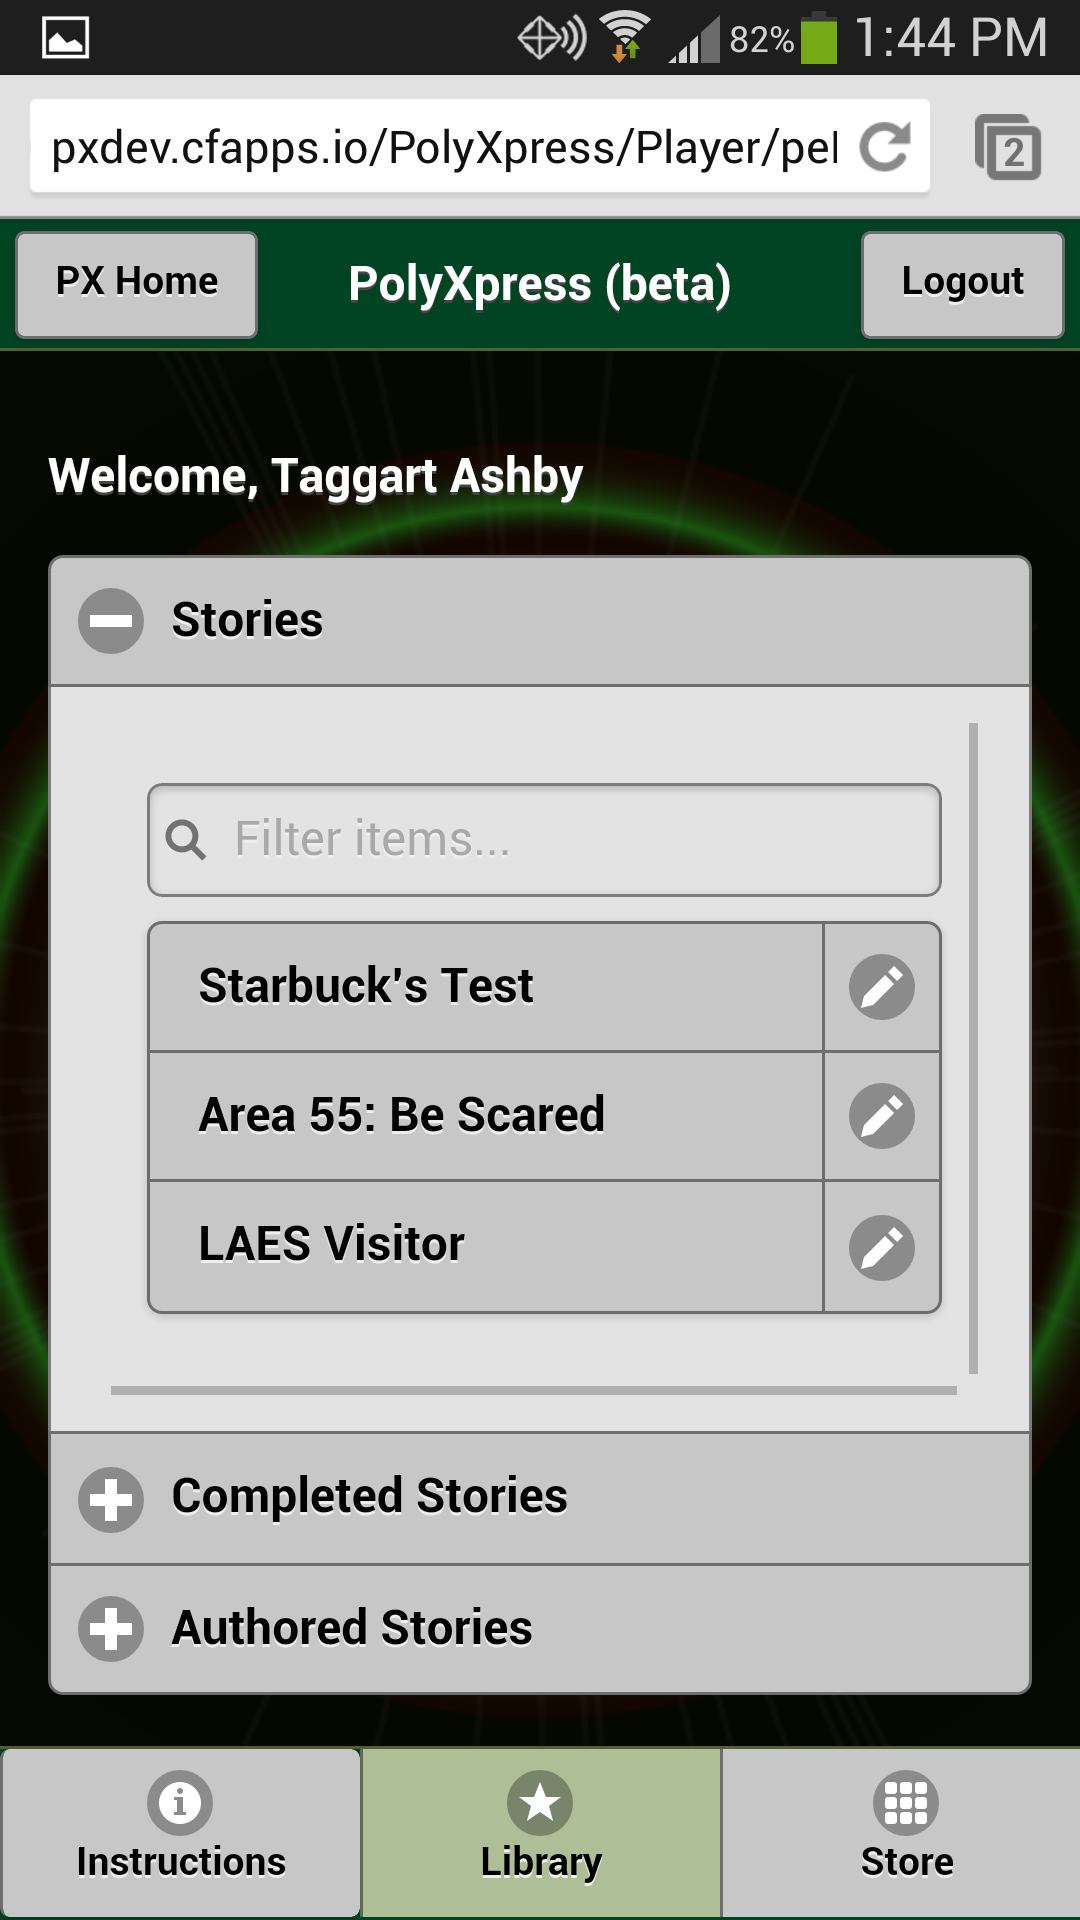
\includegraphics[width=0.30\linewidth]{px_stories.png}
  
\captionof{figure}{Story selection}

\end{Figure}

\begin{Figure}
  \centering
  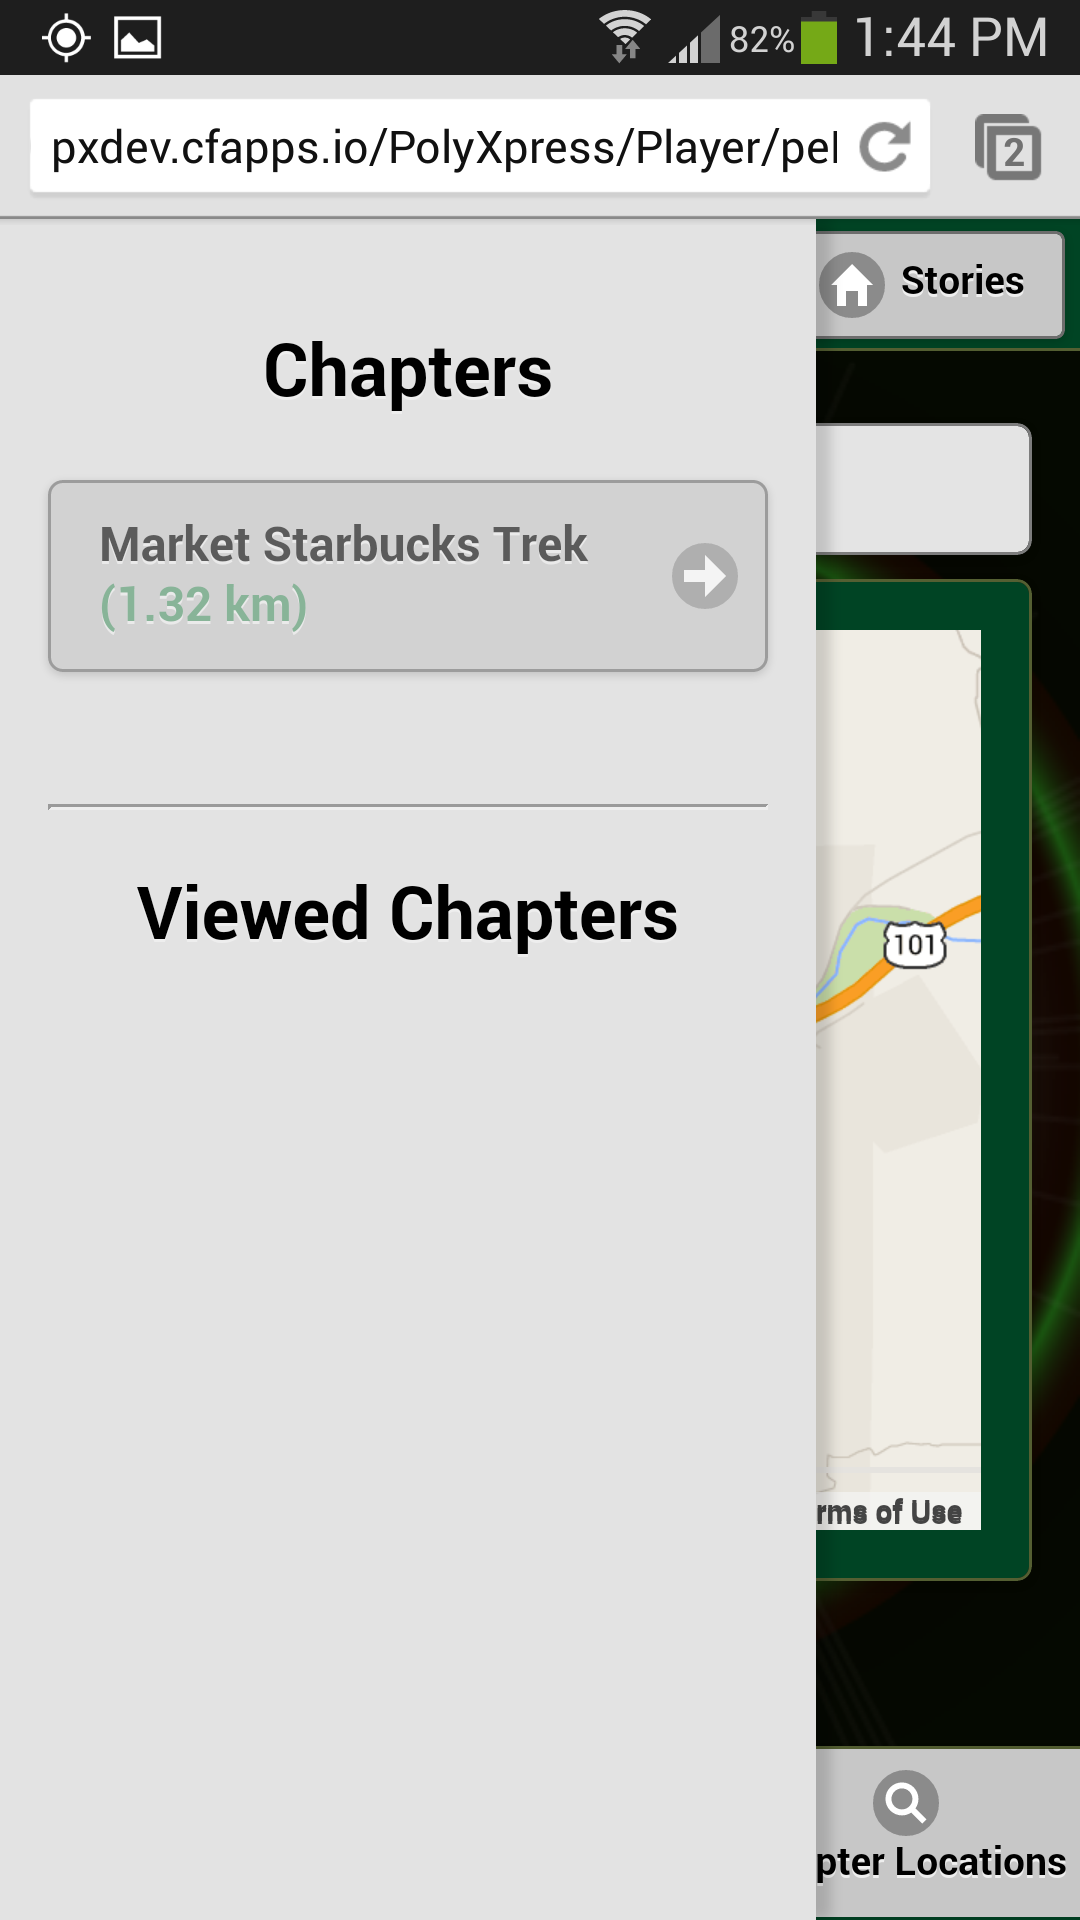
\includegraphics[width=0.30\linewidth]{px_chapter_pane.png}
  
\captionof{figure}{Chapter pane with approximate distances to each chapter}

\end{Figure}

\begin{Figure}
  \centering
  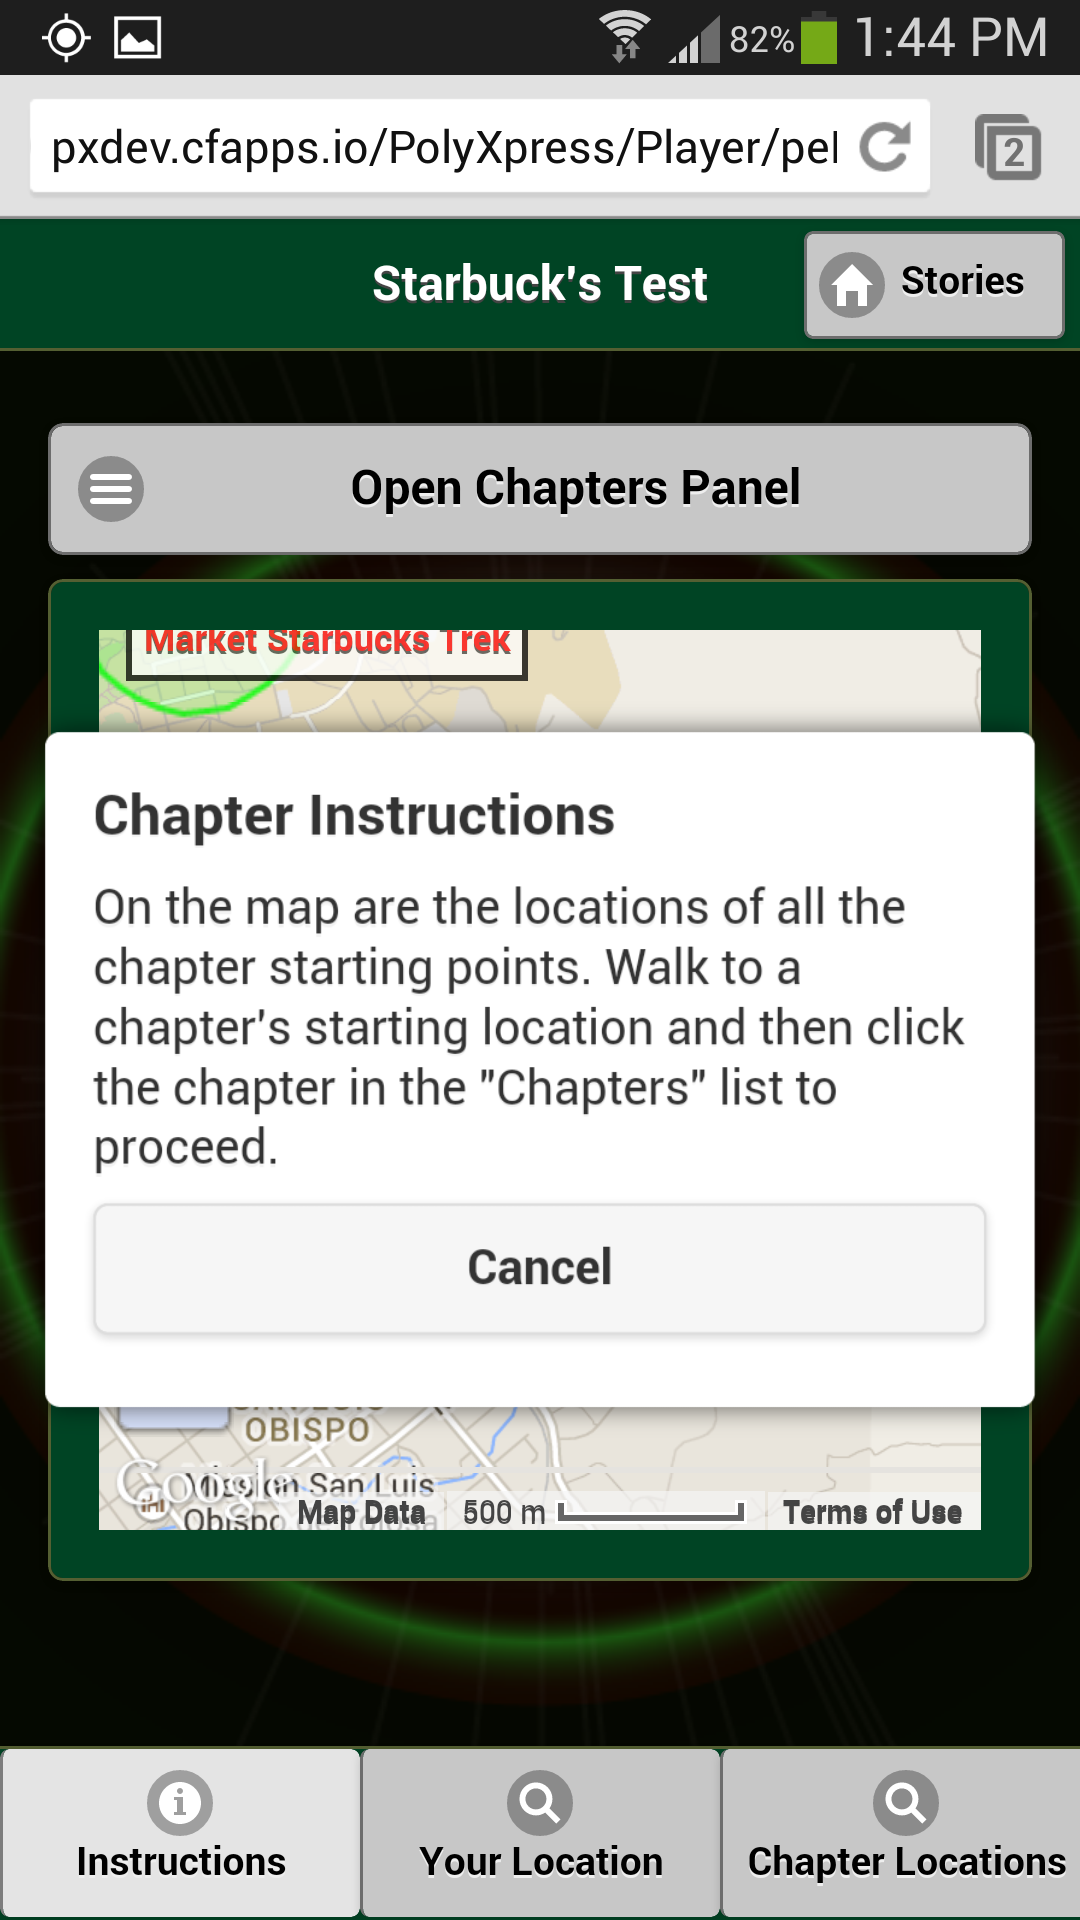
\includegraphics[width=0.30\linewidth]{px_chap_instructions.png}
  
\captionof{figure}{Each page and element of PolyXpress has instructions, here they are for Chapters}

\end{Figure}

\begin{Figure}
  \centering
  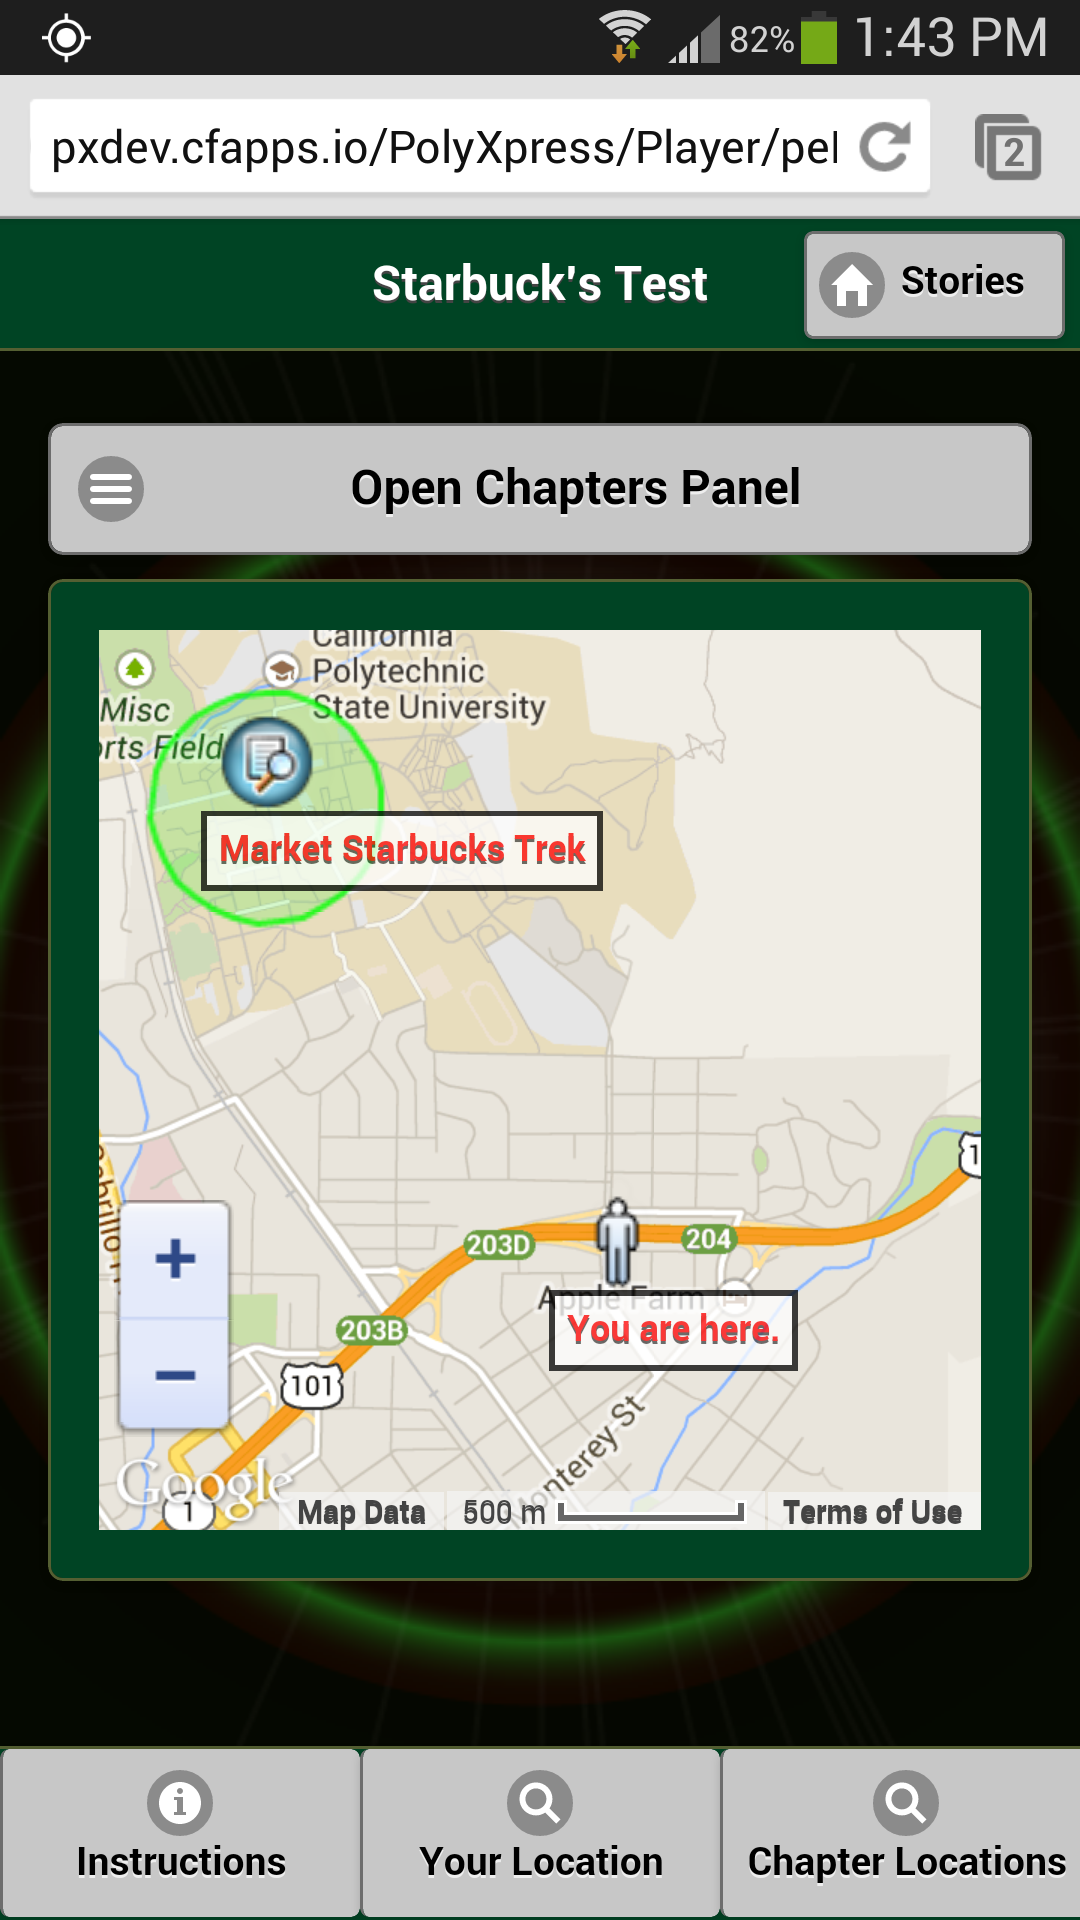
\includegraphics[width=0.30\linewidth]{px_chapter_locs.png}
  
\captionof{figure}{A map of the chapter location in relation to the player}

\end{Figure}

\begin{Figure}
  \centering
  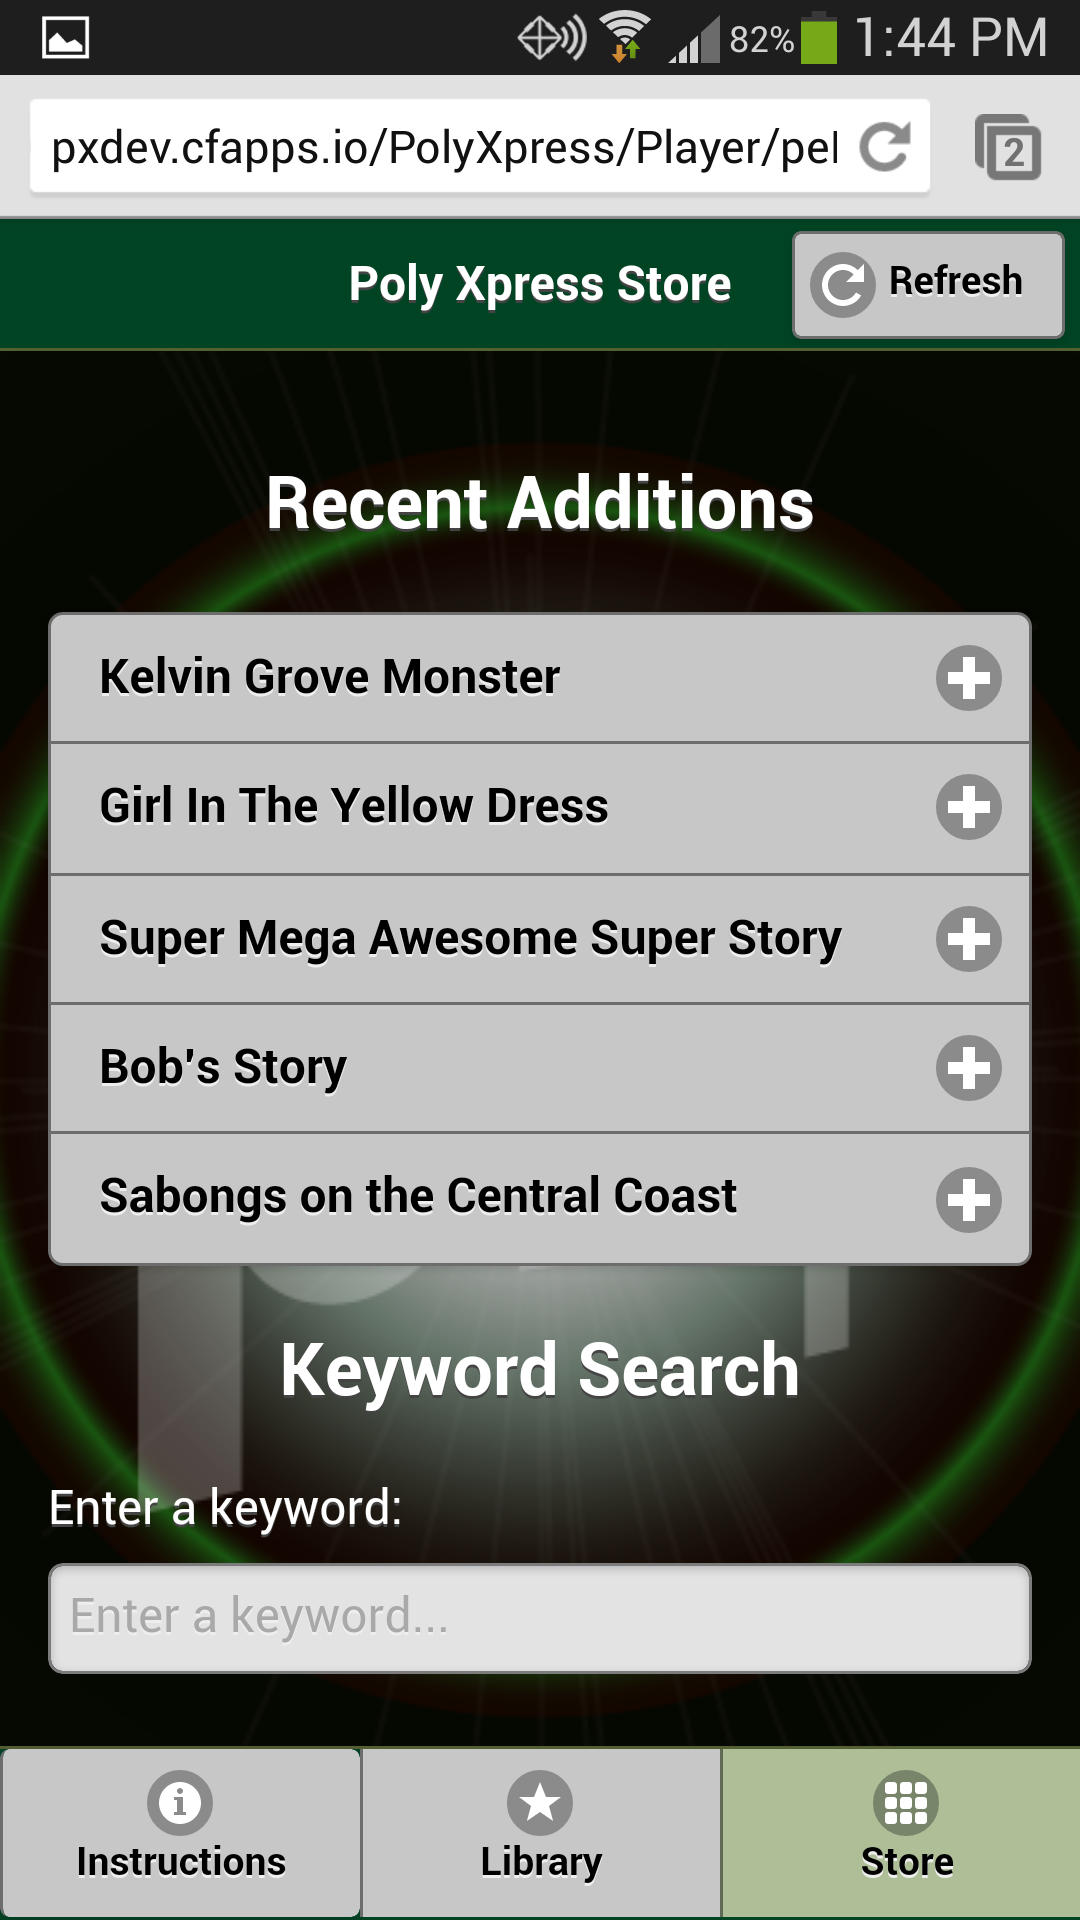
\includegraphics[width=0.30\linewidth]{px_marketplace.png}
  
\captionof{figure}{PolyXpress marketplace, to find other published stories}

\end{Figure}

\begin{Figure}
  \centering
  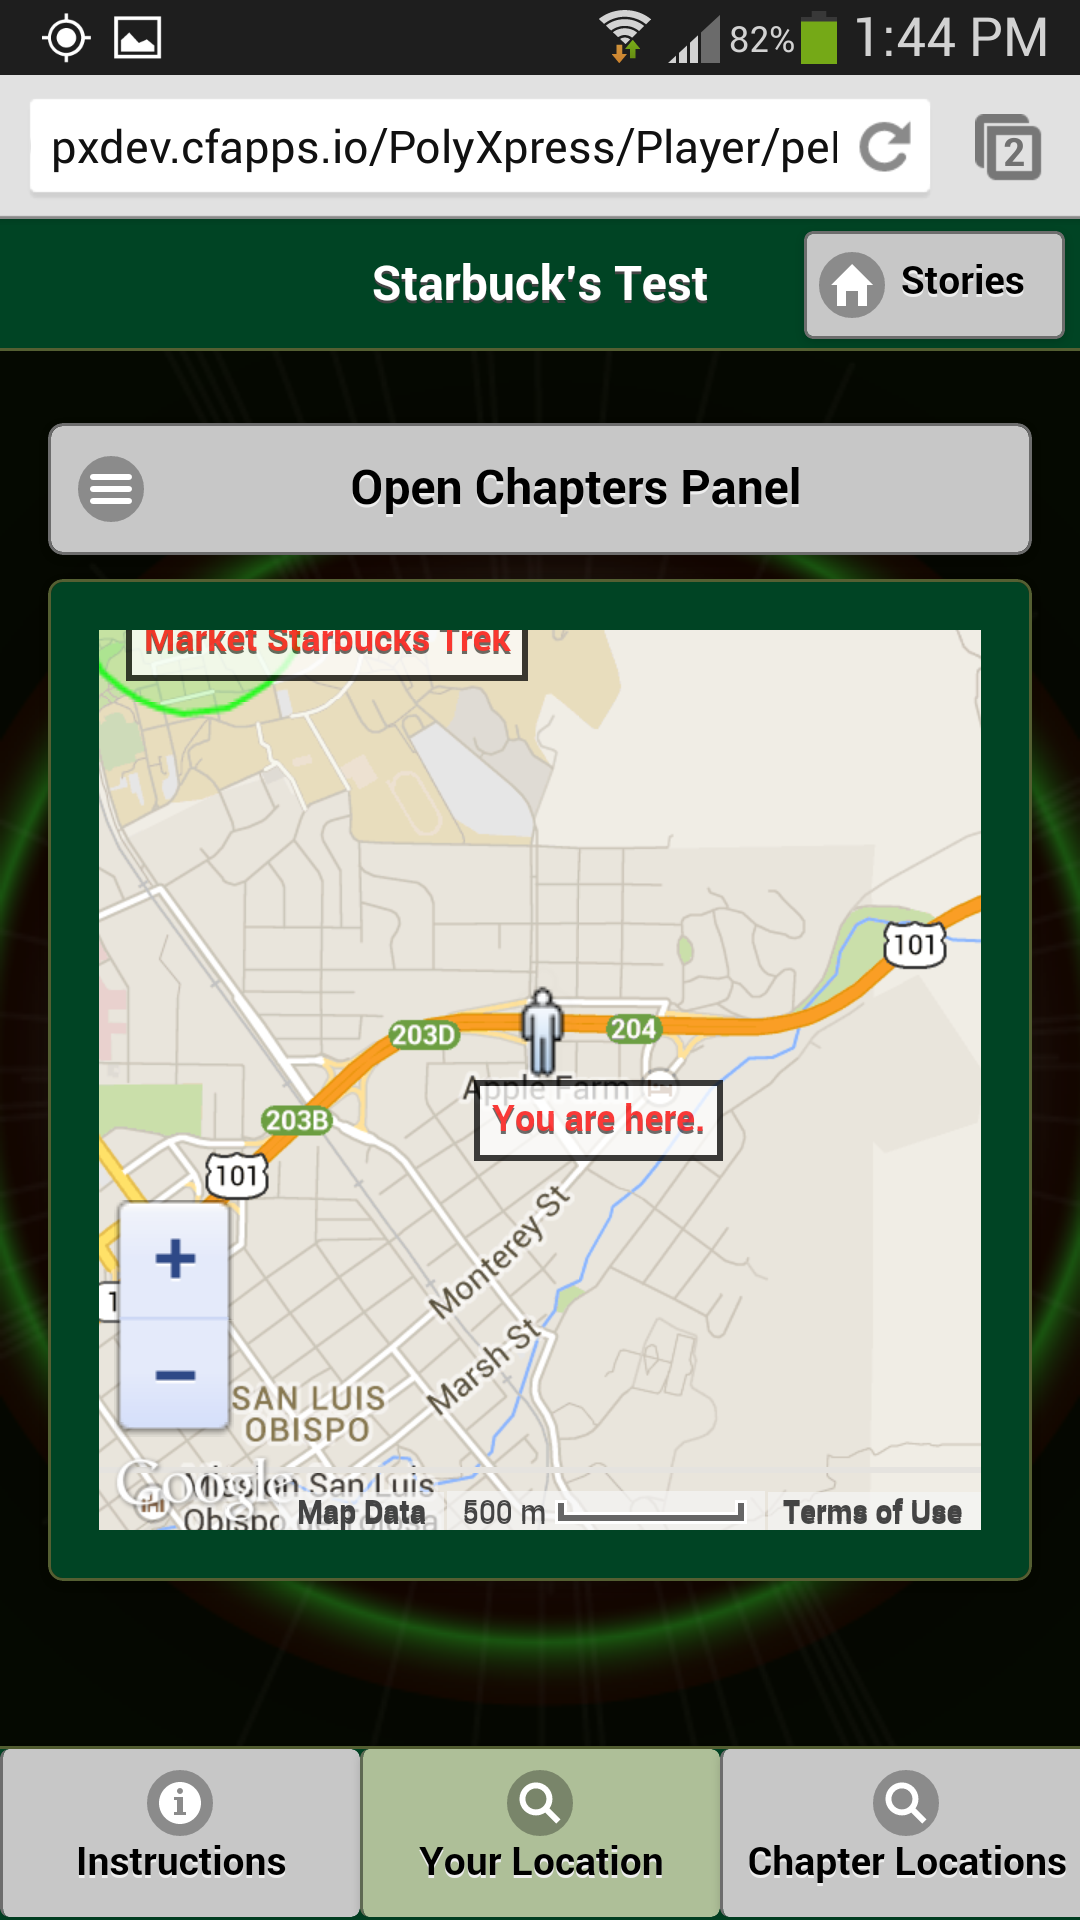
\includegraphics[width=0.30\linewidth]{px_player_loc.png}
  
\captionof{figure}{A map centered around the player}

\end{Figure}

\section{PolyXpress Author Screenshots}
\begin{Figure}
  \centering
  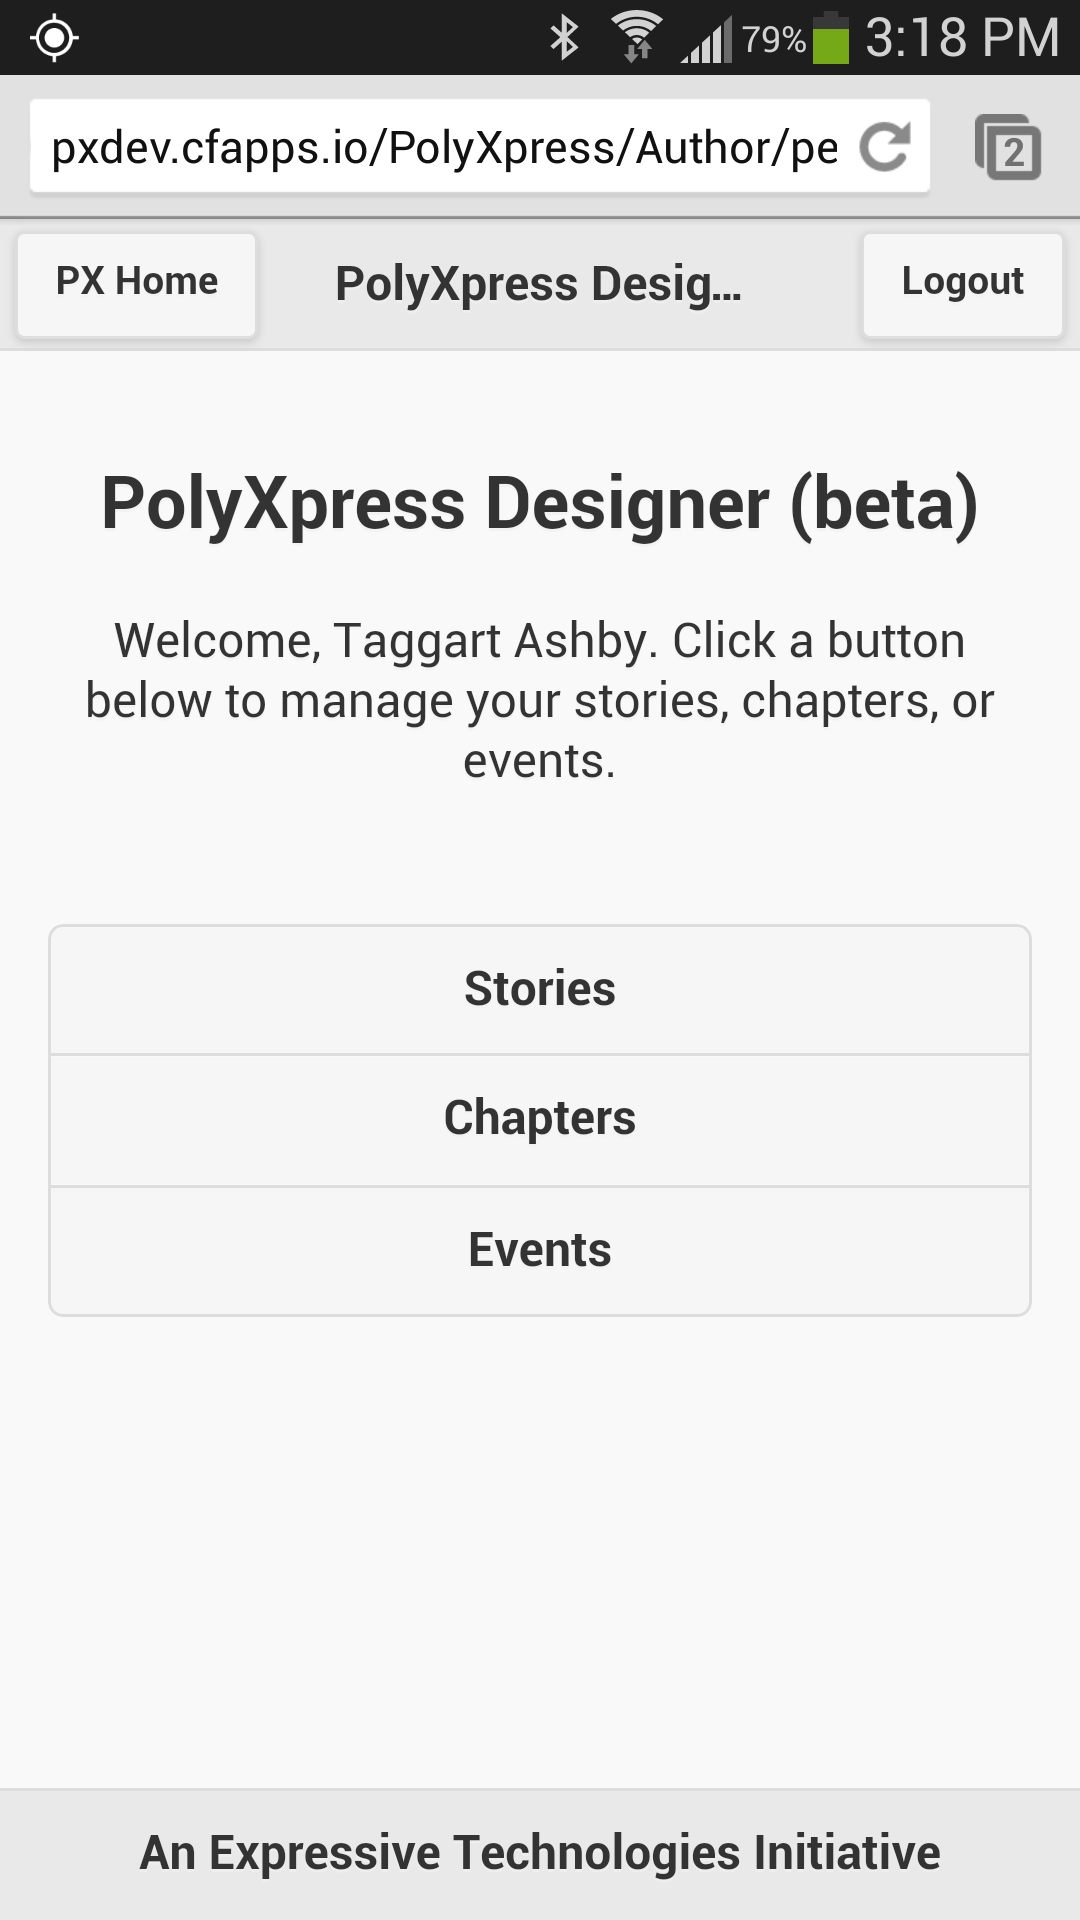
\includegraphics[width=0.30\linewidth]{px_author_home.png}
  
\captionof{figure}{PolyXpress Authoring Tool}

\end{Figure}

\begin{Figure}
  \centering
  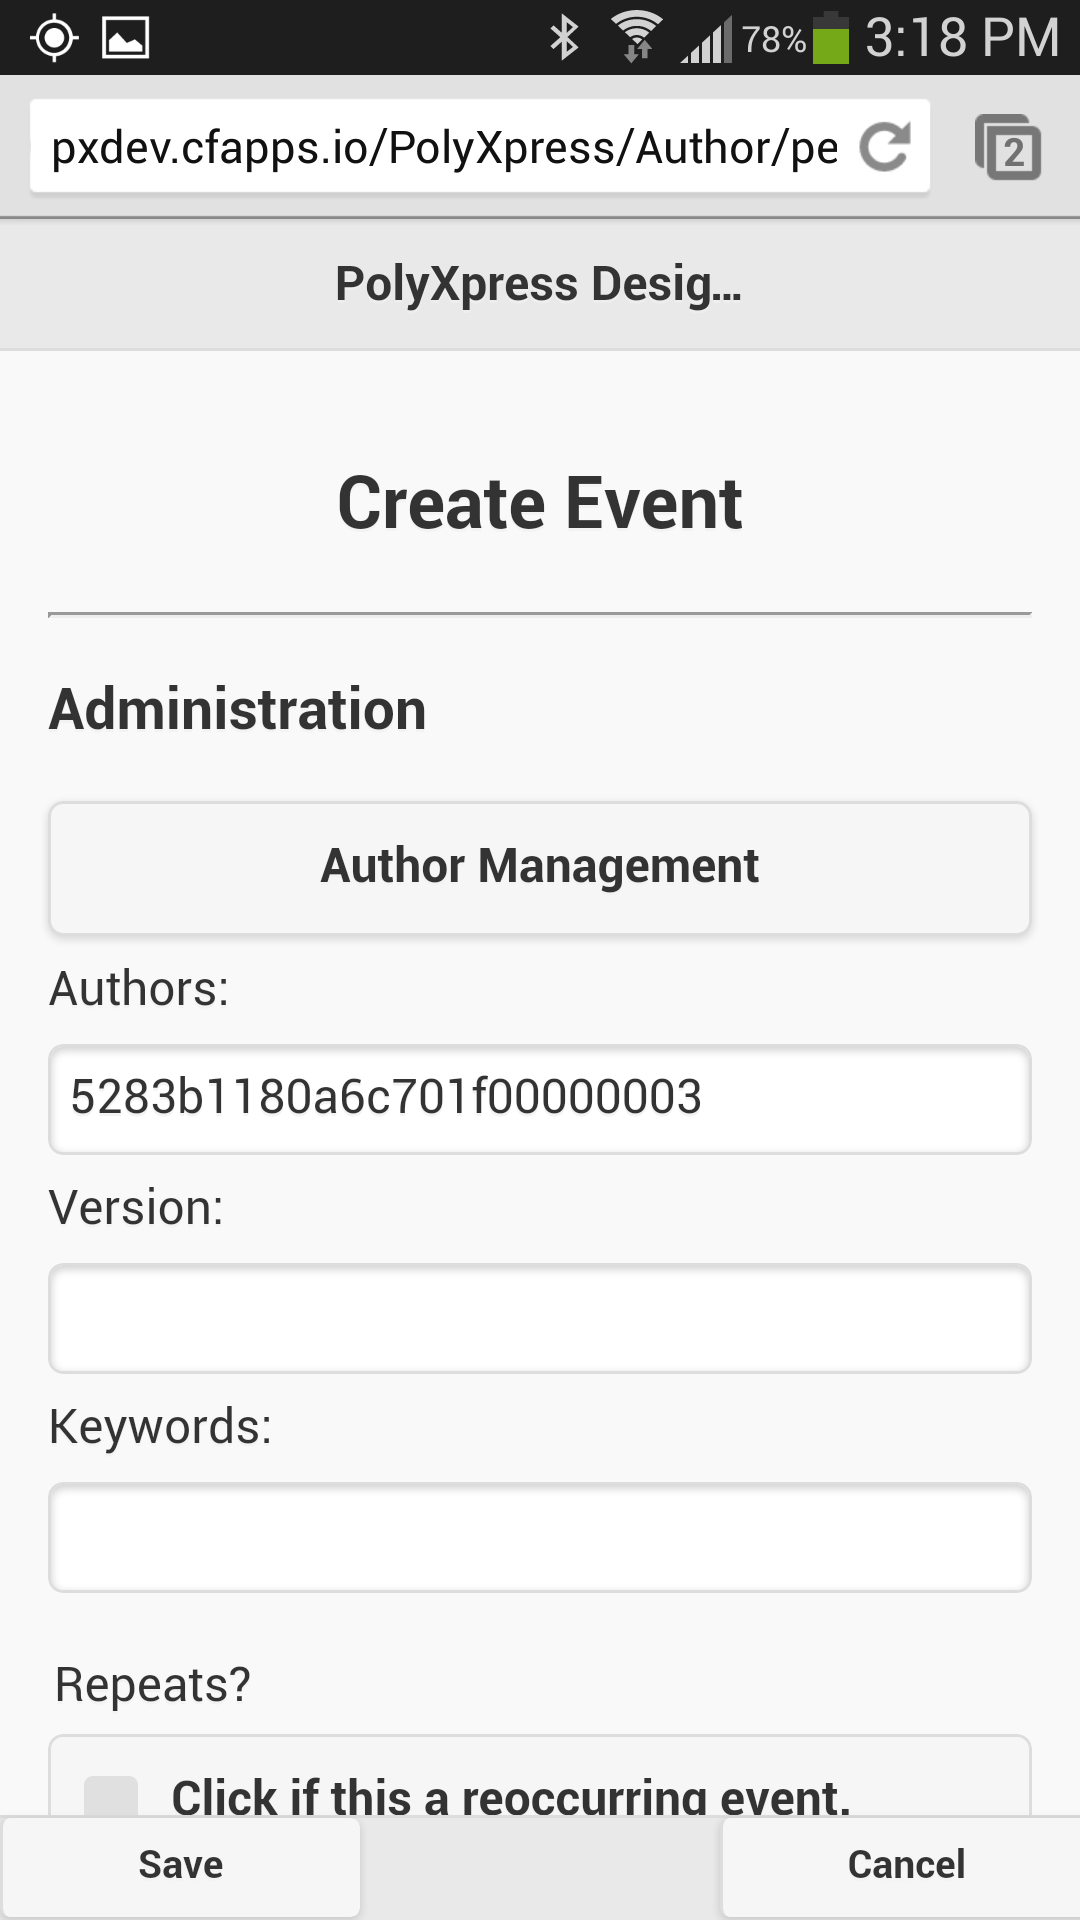
\includegraphics[width=0.30\linewidth]{px_create_event.png}
  
\captionof{figure}{Form to create an Event}

\end{Figure}

\begin{Figure}
  \centering
  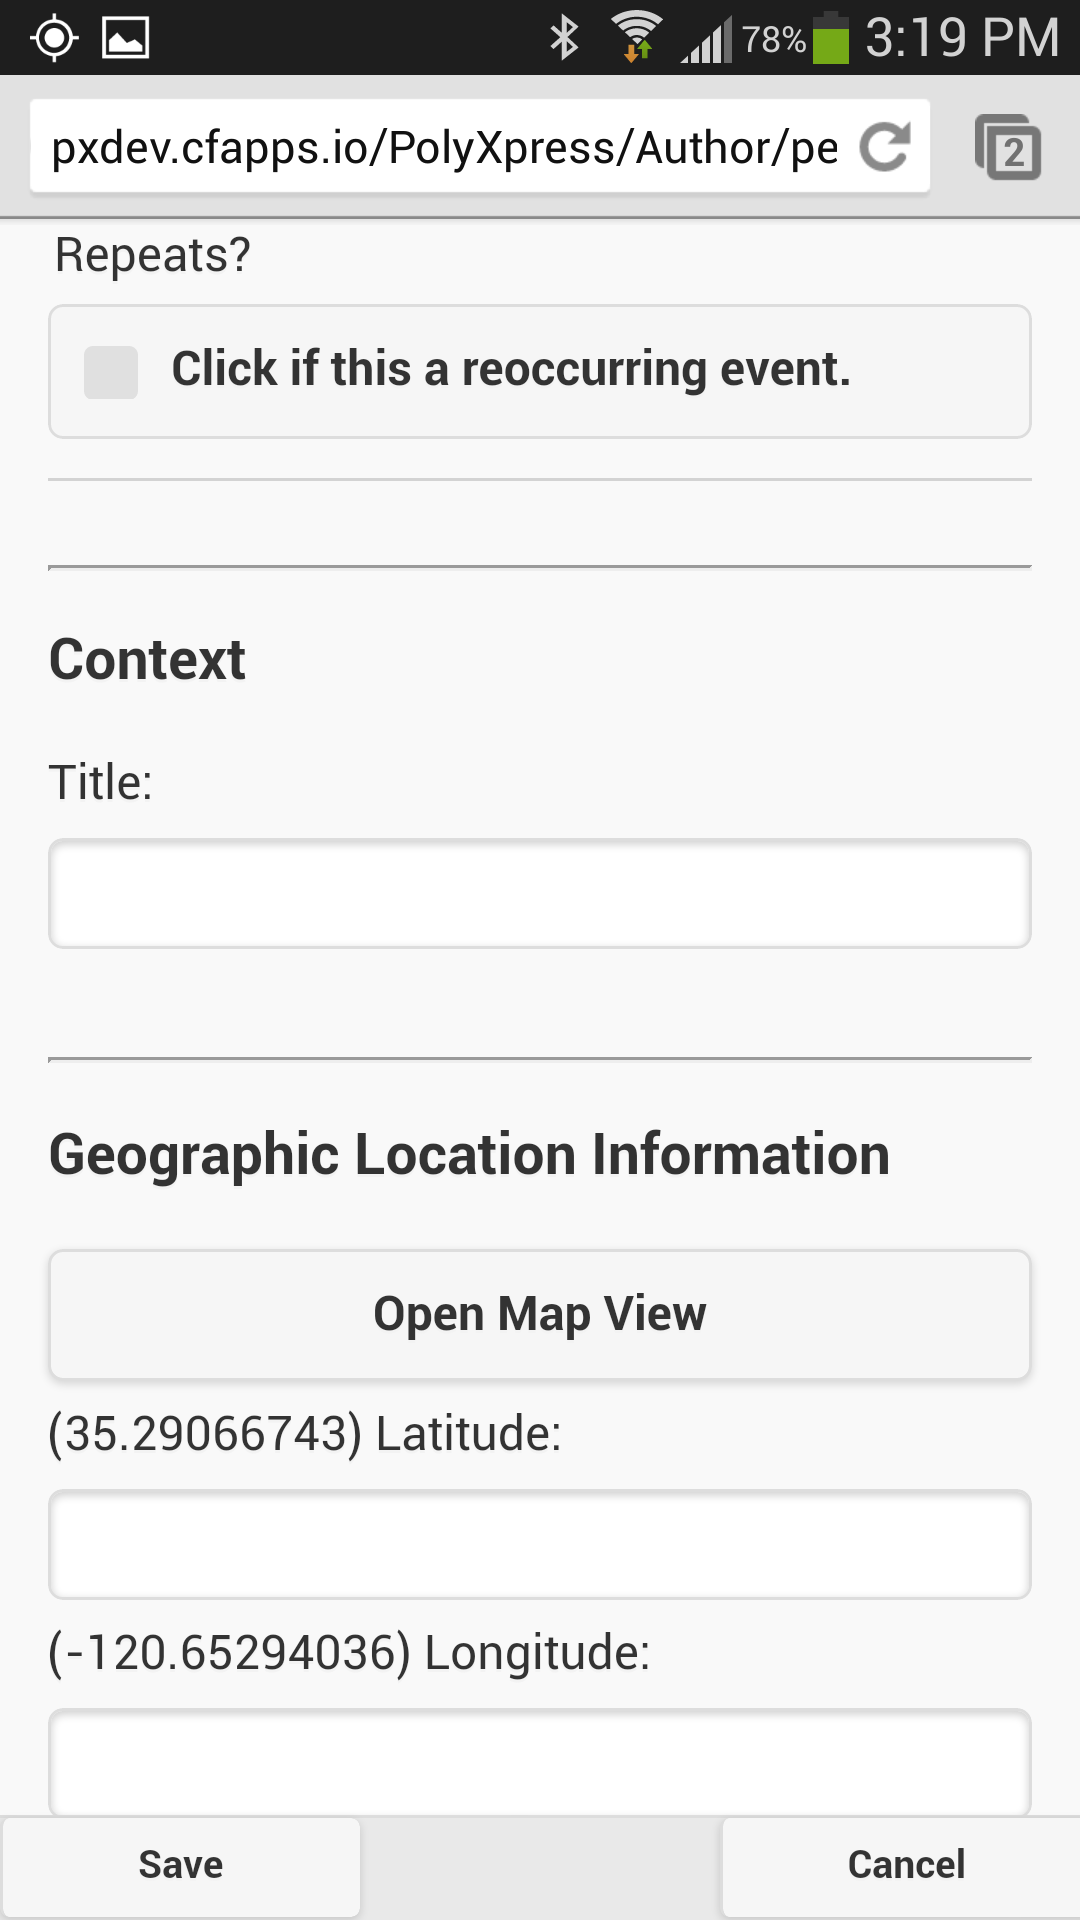
\includegraphics[width=0.30\linewidth]{px_create_event2.png}
  
\captionof{figure}{Bottom of form to create an Event}

\end{Figure}

\begin{Figure}
  \centering
  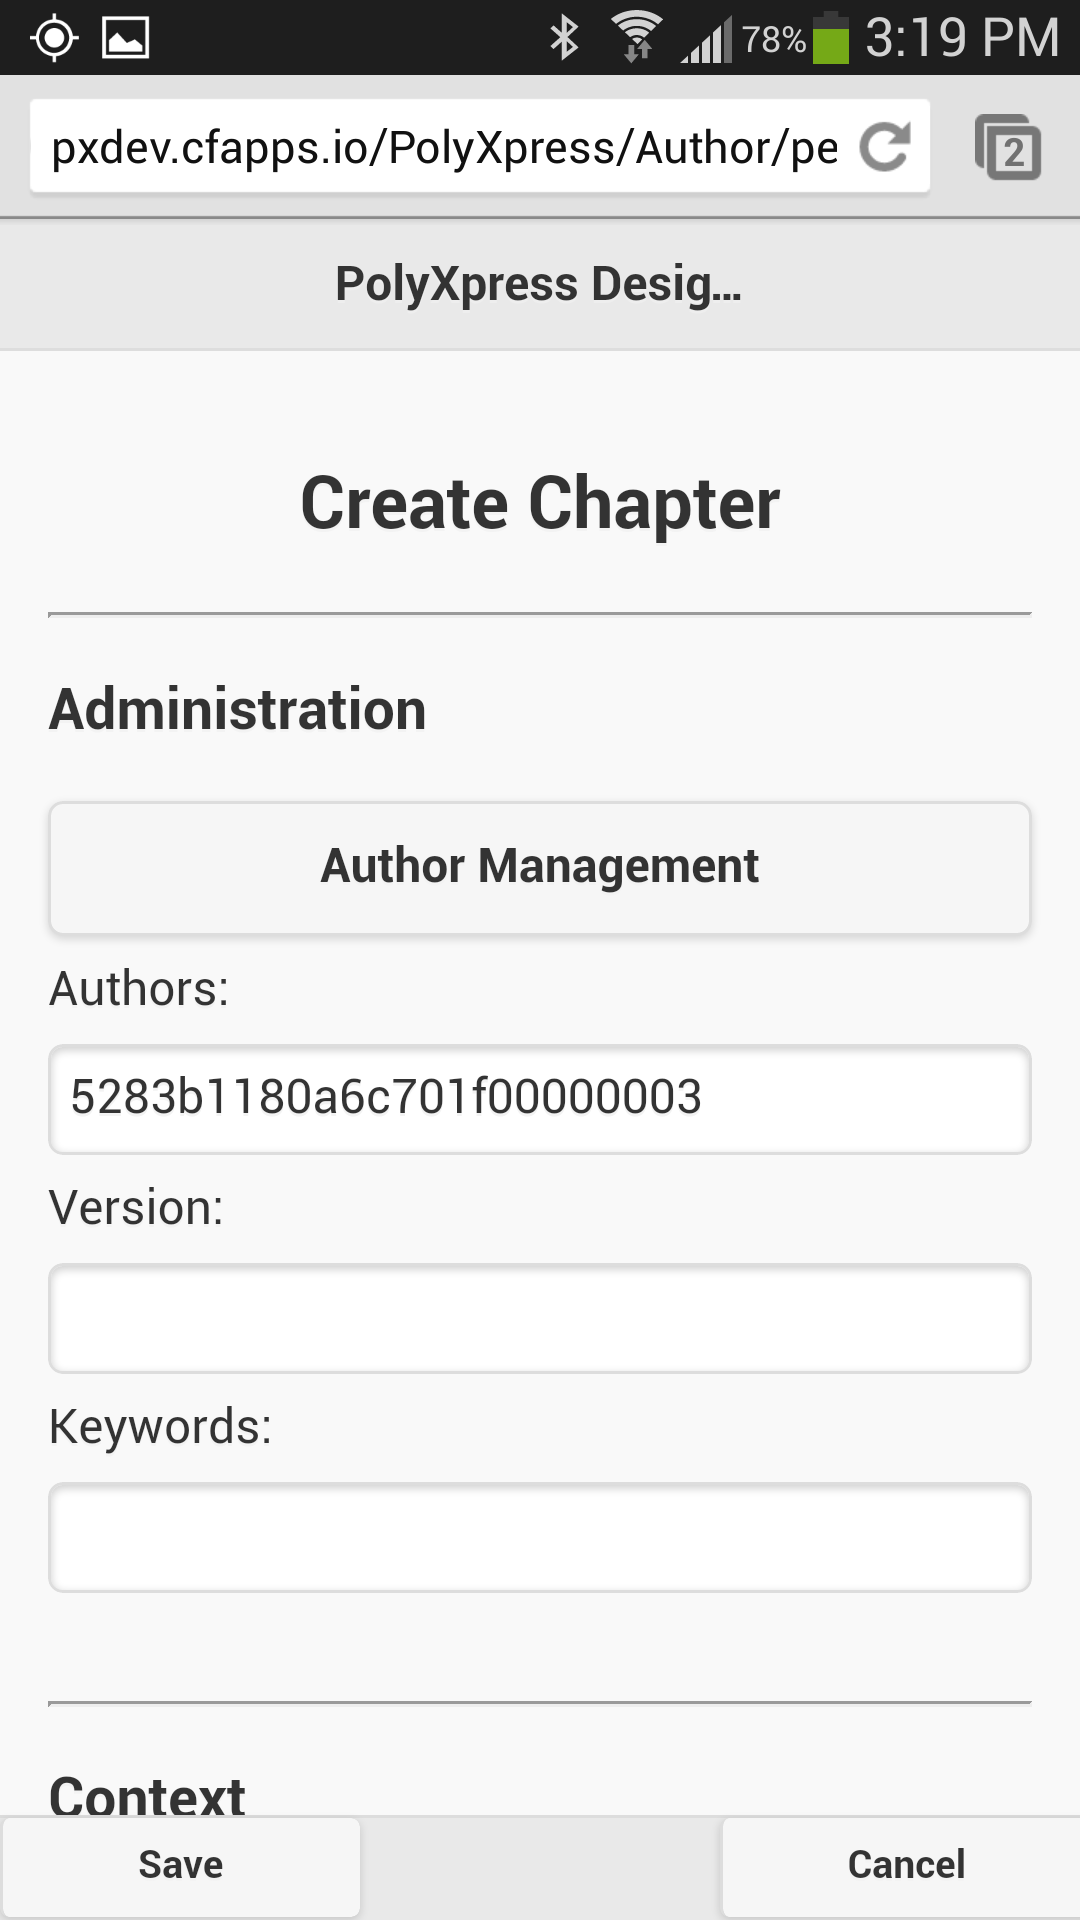
\includegraphics[width=0.30\linewidth]{px_create_chap.png}
  
\captionof{figure}{Form for creating Chapters}

\end{Figure}

\begin{Figure}
  \centering
  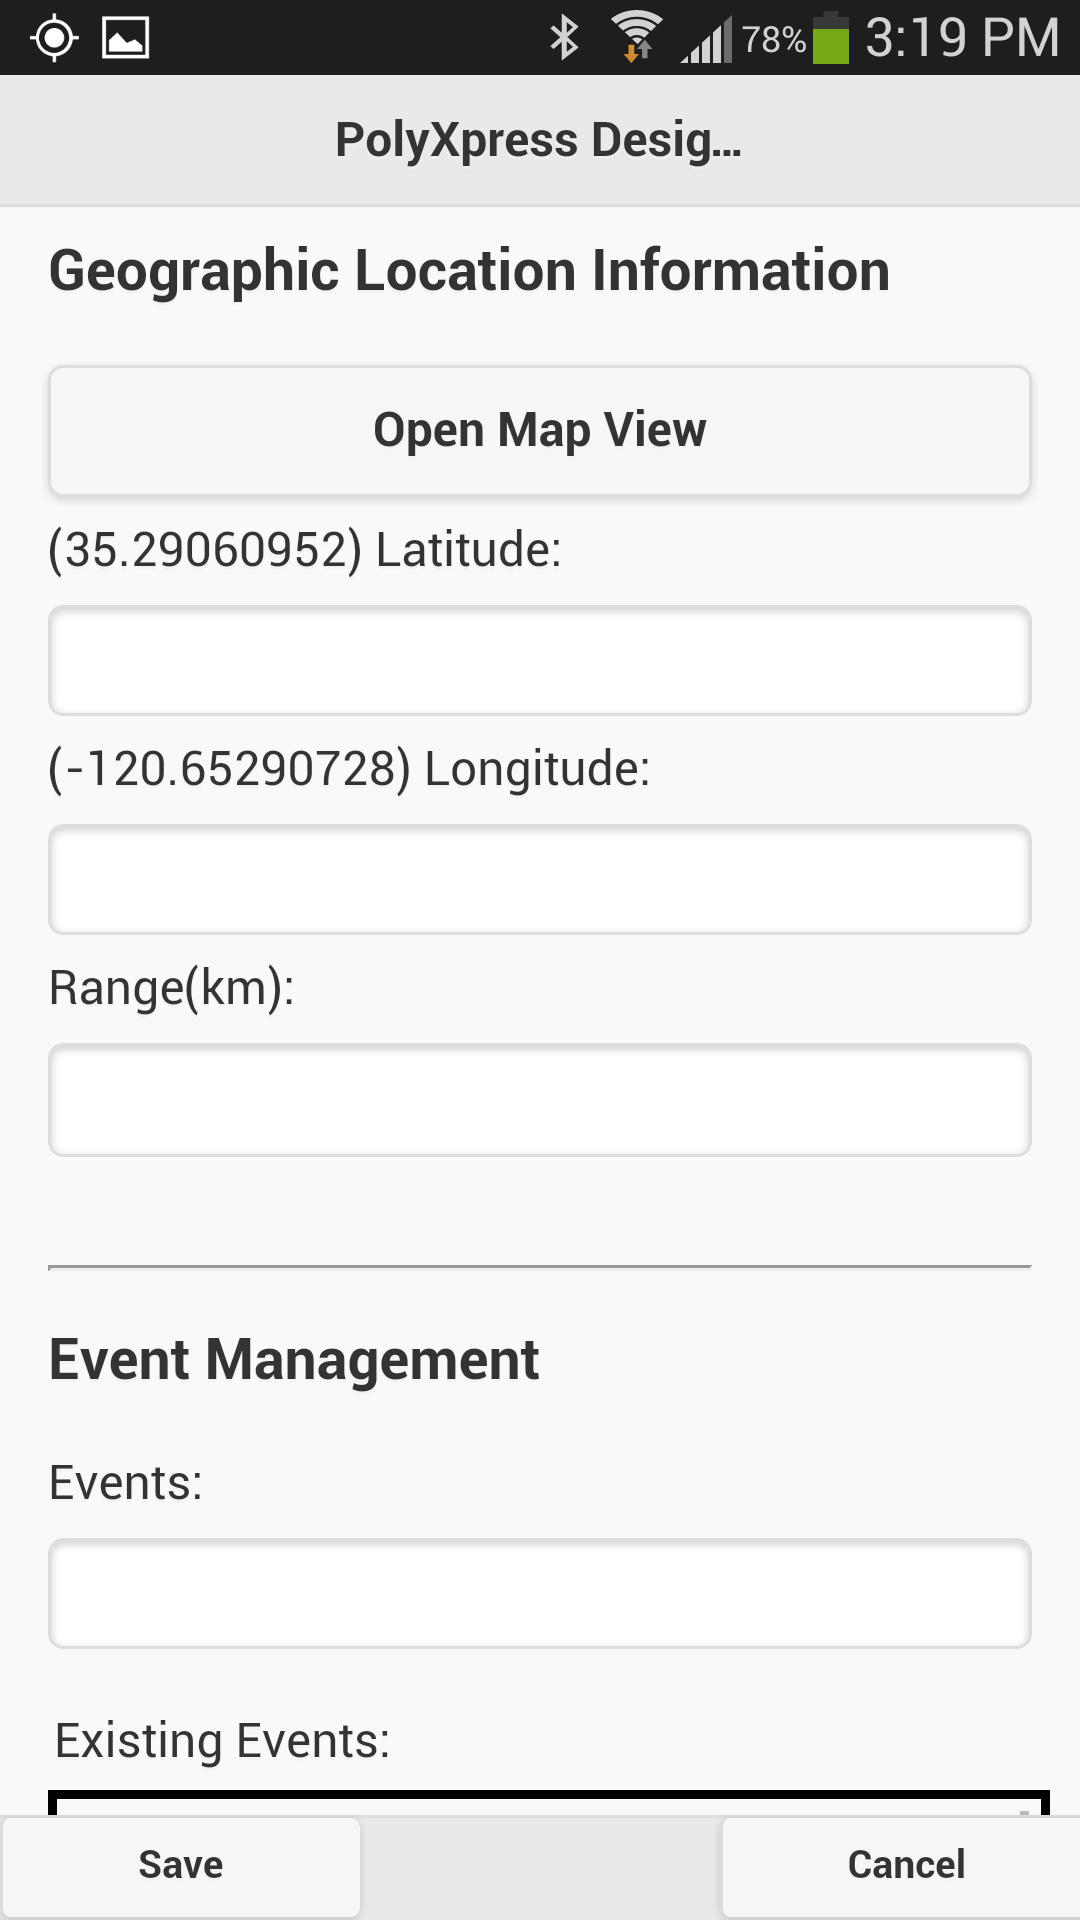
\includegraphics[width=0.30\linewidth]{px_create_chap2.png}
  
\captionof{figure}{Events are selected manually for inclusion in Chapters}

\end{Figure}

\begin{Figure}
  \centering
  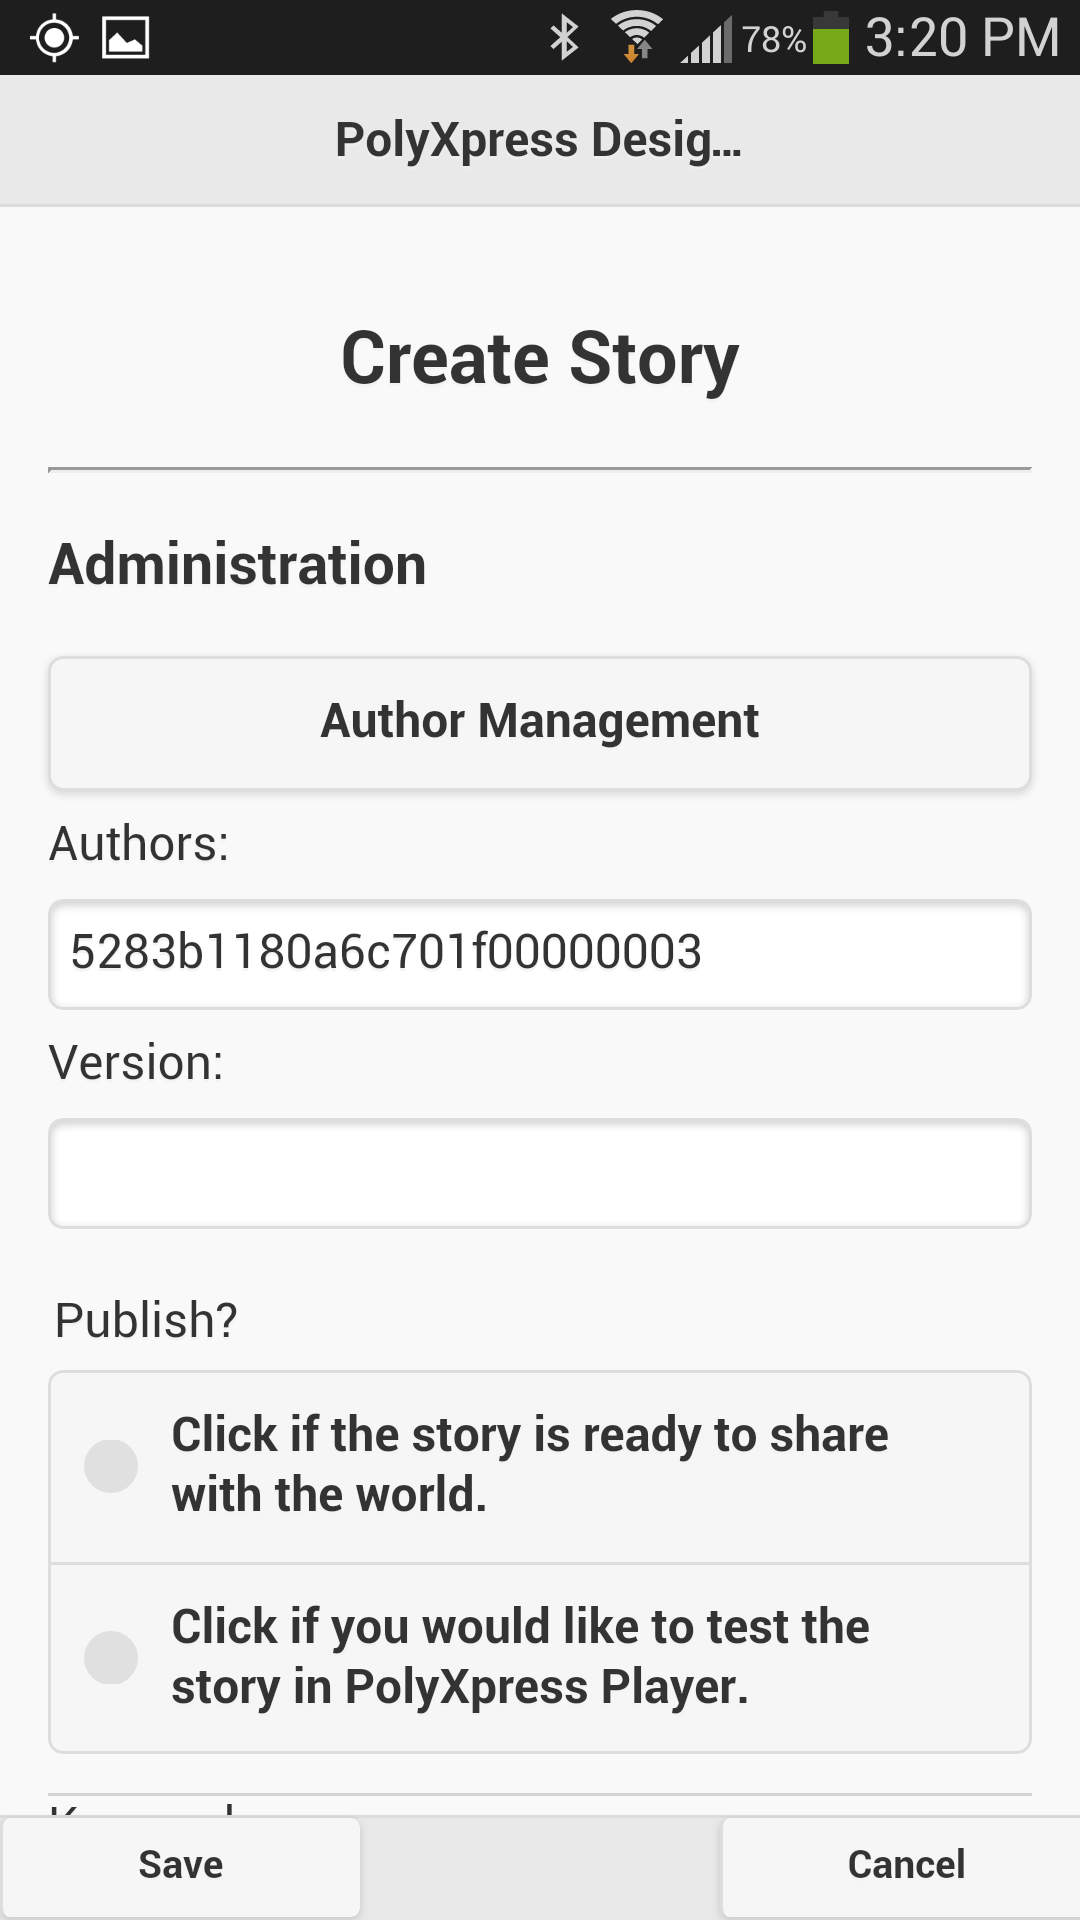
\includegraphics[width=0.30\linewidth]{px_create_story.png}
  
\captionof{figure}{Story creation asks if the user wants their story published}

\end{Figure}

% \section{PolyXpress Test Code}

% \subsection{Author Model Unit Test}
% \begin{lstlisting}
% var assert = require("chai").assert;

% describe('PX Designer Model', function() {
%     var model = require('../src/js/peDesignerModel.js')();

%     before(function() {
%         model.storyMap.push({_id: "storyID", title: "Story Test"});
%         model.chapterMap.push({_id: "chapterID", title: "Chapter Test"});
%         model.eventMap.push({_id: "eventID", title: "Event Test"});
%     });
    
%     after(function() {
%     });

%     /* Object Methods */

%     describe('stories', function () {
%       it('should be found by ID', function() {
%           // findStoryByID
%           assert.equal(model.findStoryByID("storyID").title, "Story Test");
%       });
      
%       it('should not be found by bogus ID', function() {
%           // findStoryByID
%           assert.isUndefined(model.findStoryByID("bogusID")); 
%       });

%       it('should be updateable', function() {
%           // updateStory
%           var story = {_id: model.storyMap[0]._id, title: "New Story Test"};

%           model.updateStory(story);

%           assert.equal(model.storyMap[0].title, "New Story Test");
%       });

%       it('should be deleteable', function() {
%           // deleteStory
%           var storyID = model.storyMap[0]._id;

%           model.deleteStory(storyID);

%           assert.lengthOf(model.storyMap, 0);
%       });

%       it('should be able to be populated', function() {
%           // populateStoryMap
%           var stories = [{_id: "story1", title: "Story 1"}, 
%             {_id: "story2", title: "Story 2"}, 
%             {_id: "story3", title: "Story 3"}];

%           model.populateStoryMap(stories);

%           assert.lengthOf(model.storyMap, 3);

%           assert.equal(model.storyMap[0]._id, "story1");
%           assert.equal(model.storyMap[0].title, "Story 1");

%           assert.equal(model.storyMap[1]._id, "story2");
%           assert.equal(model.storyMap[1].title, "Story 2");

%           assert.equal(model.storyMap[2]._id, "story3");
%           assert.equal(model.storyMap[2].title, "Story 3");
%       });
%     });
    
%     describe('chapters', function () {
%       it('should be found by ID', function() {
%           // findChapterByID
%           assert.equal(model.findChapterByID("chapterID").title, "Chapter Test");
%       });
      
%       it('should not be found by bogus ID', function() {
%           // findChapterByID
%           assert.isUndefined(model.findChapterByID("bogusID")); 
%       });

%       it('should be updateable', function() {
%           // updateChapter
%           var chapter = {_id: model.chapterMap[0]._id, title: "New Chapter Test"};

%           model.updateChapter(chapter);

%           assert.equal(model.chapterMap[0].title, "New Chapter Test");
%       });

%       it('should be deleteable', function() {
%           // deleteChapter
%           var chapterID = model.chapterMap[0]._id;

%           model.deleteChapter(chapterID);

%           assert.lengthOf(model.chapterMap, 0);
%       });

%       it('should be able to be populated', function() {
%           // populateChapterMap
%           var chapters = [{_id: "chapter1", title: "Chapter 1"}, 
%             {_id: "chapter2", title: "Chapter 2"}, 
%             {_id: "chapter3", title: "Chapter 3"}];

%           model.populateChapterMap(chapters);

%           assert.lengthOf(model.chapterMap, 3);

%           assert.equal(model.chapterMap[0]._id, "chapter1");
%           assert.equal(model.chapterMap[0].title, "Chapter 1");

%           assert.equal(model.chapterMap[1]._id, "chapter2");
%           assert.equal(model.chapterMap[1].title, "Chapter 2");

%           assert.equal(model.chapterMap[2]._id, "chapter3");
%           assert.equal(model.chapterMap[2].title, "Chapter 3");
%       });
%     });


%     describe('events', function () {
%       it('should be found by ID', function() {
%           // findEventByID
%           assert.equal(model.findEventByID("eventID").title, "Event Test");
%       });
      
%       it('should not be found by bogus ID', function() {
%           // findEventByID
%           assert.isUndefined(model.findEventByID("bogusID")); 
%       });

%       it('should be updateable', function() {
%           // updateEvent
%           var updated_event = {_id: model.eventMap[0]._id, title: "New Event Test"};

%           model.updateEvent(updated_event);

%           assert.equal(model.eventMap[0].title, "New Event Test");
%       });

%       it('should be deleteable', function() {
%           // deleteEvent
%           var eventID = model.eventMap[0]._id;

%           model.deleteEvent(eventID);

%           assert.lengthOf(model.eventMap, 0);
%       });

%       it('should be able to be populated', function() {
%           // populateEventMap
%           var events = [{_id: "event1", title: "Event 1"}, 
%             {_id: "event2", title: "Event 2"}, 
%             {_id: "event3", title: "Event 3"}];

%           model.populateEventMap(events);

%           assert.lengthOf(model.eventMap, 3);

%           assert.equal(model.eventMap[0]._id, "event1");
%           assert.equal(model.eventMap[0].title, "Event 1");

%           assert.equal(model.eventMap[1]._id, "event2");
%           assert.equal(model.eventMap[1].title, "Event 2");

%           assert.equal(model.eventMap[2]._id, "event3");
%           assert.equal(model.eventMap[2].title, "Event 3");
%       });
%     });
% });
% \end{lstlisting}

% \subsection{Author Controller Unit Test}
% \begin{lstlisting}
% var assert = require('chai').assert;

% controllerStubs = {
%   elements: {},
%   createdElements: {}
% };

% // Stub
% document = {
%   getElementById: function (elementName) {
%     controllerStubs.elements[elementName] = {
%       name: elementName,
%       style: '',
%       firstChild: undefined,
%       children: [],
%       appendChild: function (child) {
%         this.children.push(child);
%         this.firstChild = child;
%       },
%       removeChild: function (child) {
%         if (this.children.length > 0) {
%           this.children.pop(child);
%           this.firstChild = this.children[0];
%         }
%       },
%       getElementsByTagName: function (element) {return [];}
%     }
%     return controllerStubs.elements[elementName];
%   },
%   createElement: function (elementType) {
%     controllerStubs.createdElements[elementType] = {
%       type: elementType,
%       firstChild: undefined,
%       children: [],
%       appendChild: function (child) {
%         this.children.push(child);
%         this.firstChild = child;
%       },
%       removeChild: function (child) {
%         if (this.children.length > 0) {
%           this.children.pop(child);
%           this.firstChild = this.children[0];
%         }
%       },
%       setAttribute: function (att, val) {}
%     }

%     return controllerStubs.createdElements[elementType];
%   },
%   createTextNode: function (text) {
%     return {
%       text: text
%     }
%   }
% };

% confirm = function (_) {return true};

% createStory = {
%   title: {}, authors: {}, version: {}, publish: {}, test: {}, 
%   keywords:{}, overview: {}, image: {}, music: {}, chapters: {}
% };

% createChapter = {
%   ctitle: {}, cauthors: {}, cversion: {}, ckeywords: {}, coverview: {},
%   cimage: {}, cmusic: {}, clat: {}, clng: {}, crange: {}, cevents: {}
% }

% createEvent = {
%   etitle: {}, eauthors: {}, eversion: {}, ekeywords: {},
%   erepeats: {}, elat: {}, elng: {}, erange: {}
% }

% window = {};

% alert = function(message) {
%   controllerStubs.alertMsg = message;
% }

% // Stub for JQM initialization in peDesignerController
% $ = function (_) {
%   return {
%     on: function (event, element, callback) {
%       controllerStubs.event = event;
%       controllerStubs.element = element;
%       controllerStubs.callback = callback;
%     },
%     trigger: function (event) {
%       controllerStubs.event = event;
%       controllerStubs.element = _;
%     },
%     checkboxradio: function (_) {},
%     hasClass: function (_) {},
%     listView: function (_) {}
%   }
% }

% $.mobile = {
%   changePage: function(newPage) {}
% }

% map_canvas = "map canvas";
% google = {maps: {event: {}}};
% google.maps.event.trigger = function (element, action) {
%   controllerStubs.google = {element: element, action: action};
% }

% // Need to overwrite peDesignerServer calls to isolate controller
% controllerDS = {
%   getAuthorData: function (authorDataCallback) {
%     this.authorData = {name: "controllerDS Author Data", _id: 0};
%     controllerStubs.controllerDSCall = true;

%     authorDataCallback(this.authorData);
%   },
%   submitNewStory: function(storyData, authorData, storyCallback) {
%     controllerDS.newStory = {storyData: storyData, authorData: authorData}
%   },
%   submitUpdateStory: function(storyID, storyData, storyCallback) {
%     controllerDS.updateStory = {storyID: storyID, storyData: storyData}
%   },
%   submitDeleteStory: function(updateStoryID, authorData, populateStoryList) {},
%   submitNewChapter: function(chapterData, authorData, chapterCallback) {
%     controllerDS.newChapter = {chapterData: chapterData, authorData: authorData}
%   },
%   submitUpdateChapter: function(chapterID, chapterData, chapterCallback) {
%     controllerDS.updateChapter = {chapterID: chapterID, chapterData: chapterData}
%   },
%   submitDeleteChapter: function(updateChapterID, authorData, populateChapterList) {},
%   submitNewEvent: function(eventData, eventCallback) {
%     controllerDS.newEvent = {eventData: eventData}
%   },
%   submitUpdateEvent: function(eventID, eventData, eventCallback) {
%     controllerDS.updateEvent = {eventID: eventID, eventData: eventData}
%   },
%   submitDeleteEvent: function(updateEventID, authorData, populateEventList) {}
% };

% controllerDM = {
%   storyMap: [
%     // First story built out to accomodate all tests
%     {title: 'Test Story 1', _id: '1', chapterList: [1, 2], keywords: ["test1", "test2"]}, 
%     {title: 'Test Story 2', _id: '2'}, 
%     {title: 'Test Story 3', _id: '3'}
%   ],
%   chapterMap: [
%     {title: 'Test Chapter 1', _id: '1', eventList: [1, 2], keywords: ["kw1", "kw2"], proximity: {}},
%     {title: 'Test Chapter 2', _id: '2'},
%     {title: 'Test Chapter 3', _id: '3'}
%   ],
%   eventMap: [
%     {title: 'Test Event 1', _id: '1', assetList: [{order: "Test Order 1", format: "Test Format 1", uri: "Test Data 1"}], keywords: ["kw1", "kw2"], proximity: {}},
%     {title: 'Test Event 2', _id: '2'},
%     {title: 'Test Event 3', _id: '3'}
%   ],
%   findStoryByID: function (id) {return this.storyMap[id - 1];},
%   findChapterByID: function (id) {return this.chapterMap[id - 1];},
%   findEventByID: function (id) {return this.eventMap[id - 1];}
% };

% // Test Spec Begins
% describe('PX Designer Controller', function () {
%   var controller = require('../src/js/peDesignerController.js')(controllerDS, controllerDM);

%   before(function () {
%     // For JQM Initialize
%     assert.equal(controllerStubs.event, 'pageshow');
%     assert.equal(controllerStubs.element, '#mapView');

%     controllerStubs.callback();
%     assert.equal(controllerStubs.google.element, 'map canvas');
%     assert.equal(controllerStubs.google.action, 'resize');
%   });

%   // // Documentation says unused, test here for future use, unfinished
%   // it('should set up page event handlers', function () {
%   //  // setupPageEventHandlers
%   //  assert.equal(controllerStubs.element, 'pageinit');
%   //  assert.equal(controllerStubs.event, '#mainMenu');

%   //  controllerStubs.callback();
%   // });

%   it('should show a main menu given existing author data', function () {
%     // showMainMenu

%     // Call to controllerDS
%     controller.showMainMenu();
%     assert.equal(controller.getAuthorData().name, 'controllerDS Author Data');
%     assert.isTrue(controllerStubs.controllerDSCall);
%     controllerStubs.controllerDSCall = false;

%     // No call to controllerDS
%     controller.showMainMenu();
%     assert.equal(controller.getAuthorData().name, 'controllerDS Author Data');
%     assert.isFalse(controllerStubs.controllerDSCall);
%   });

%   describe('Story Management', function () {
%     function assertClearStory() {
%       assert.equal(createStory.title.value, "");
%             assert.equal(createStory.authors.value, "");
%             assert.equal(createStory.version.value, "");
%             assert.equal(createStory.publish.checked, false);
%             assert.equal(createStory.test.checked, false);
%             assert.equal(createStory.keywords.value, "");
%             assert.equal(createStory.overview.value, "");
%             assert.equal(createStory.image.value, "");
%             assert.equal(createStory.music.value, "");
%             assert.equal(createStory.chapters.value, "");
%     }

%     it('should initialize the story manager', function () {
%       // initStoryManager, just calls populateStoryList()
%       controller.initStoryManager();
      
%       // TODO: More tests here
%       var storyList = controllerStubs.elements["existingStoryList"].children;
%       assert.lengthOf(storyList, 3);
%       assert.equal(storyList[0].innerHTML, "<a href='#storyData'>Test Story 1</a>");
%       assert.equal(storyList[1].innerHTML, "<a href='#storyData'>Test Story 2</a>");
%       assert.equal(storyList[2].innerHTML, "<a href='#storyData'>Test Story 3</a>");
%     });
    
%     it('should update a story', function () {
%       // updateStory, calls populateStoryChapterList with a story
%       controller.updateStory(1); // The 'full' story or it'll be unhappy

%       var checkboxElements = controllerStubs.elements["chapterCheckboxes"].children;
%       assert.lengthOf(checkboxElements, 6); // A label and input element for each chapter associated with the story

%       var chapter1Label = checkboxElements[0].firstChild;
%       var chapter2Label = checkboxElements[2].firstChild;
%       var chapter3Label = checkboxElements[4].firstChild;

%       var chapter1Checkbox = checkboxElements[1];
%       var chapter2Checkbox = checkboxElements[3];
%       var chapter3Checkbox = checkboxElements[5];

%       assert.equal(chapter1Label.text, "ID: 1, Title: Test Chapter 1");
%       assert.equal(chapter2Label.text, "ID: 2, Title: Test Chapter 2");
%       assert.equal(chapter3Label.text, "ID: 3, Title: Test Chapter 3");
      
%       assert.isTrue(chapter1Checkbox.checked);
%       assert.isTrue(chapter2Checkbox.checked);

%       assert.isUndefined(chapter3Checkbox.checked); // Story 3 isn't a part of this chapter!
%     });

%     it('should create a story', function () {
%       // createStory
%       controller.createStory();

%       var checkboxElements = controllerStubs.elements["chapterCheckboxes"].children;
%       assert.lengthOf(checkboxElements, 6); // A label and input element for each chapter associated with the story

%       var chapter1Label = checkboxElements[0].firstChild;
%       var chapter2Label = checkboxElements[2].firstChild;
%       var chapter3Label = checkboxElements[4].firstChild;

%       var chapter1Checkbox = checkboxElements[1];
%       var chapter2Checkbox = checkboxElements[3];
%       var chapter3Checkbox = checkboxElements[5];

%       assert.equal(chapter1Label.text, "ID: 1, Title: Test Chapter 1");
%       assert.equal(chapter2Label.text, "ID: 2, Title: Test Chapter 2");
%       assert.equal(chapter3Label.text, "ID: 3, Title: Test Chapter 3");
      
%       // A new story has no chapter boxes checked
%       assert.isUndefined(chapter1Checkbox.checked);
%       assert.isUndefined(chapter2Checkbox.checked);
%       assert.isUndefined(chapter3Checkbox.checked);
%     });

%     it('should submit a story', function () {
%       // submitStoryData
%       // Not the greatest because it relies on createStory and updateStory, but I can't change updateStoryID any other way, it's a private variable

%       // A brand new story
%       controller.createStory();

%       createStory.title.value = "New Story";
%       createStory.authors.value = "Author1 Author2";
%       createStory.chapters.value = "0 1";

%       controller.submitStoryData();

%       assert.equal(controllerDS.newStory.storyData.title, "New Story");
%       assert.deepEqual(controllerDS.newStory.storyData.authors, ["Author1", "Author2"]);
%       assert.deepEqual(controllerDS.newStory.storyData.chapterList, ["0", "1"]);

%       assert.equal(controllerStubs.alertMsg, "Adding story to server. \nHit \"ok\" to return to main menu!");

%       // Updates to a previous story
%       controller.updateStory(1);

%       createStory.title.value = "Updated Story";
%       createStory.authors.value = "Author3 Author4";
%       createStory.chapters.value = "1 2"; 

%       controller.submitStoryData();

%       assert.equal(controllerDS.updateStory.storyData.title, "Updated Story");
%       assert.deepEqual(controllerDS.updateStory.storyData.authors, ["Author3", "Author4"]);
%       assert.deepEqual(controllerDS.updateStory.storyData.chapterList, ["1", "2"]);

%       assert.equal(controllerStubs.alertMsg, "Updating story on server. \nHit \"ok\" to return to main menu!");
%     });

%     it('should validate a story', function () {
%       // validateStoryPublish
%       createStory.publish.checked = true;

%       // Invalid, no chapters
%       createStory.chapters.value = "";

%       assert.isFalse(controller.validateStoryPublish(undefined)); // Takes event param that isn't used

%       // Invalid, no events
%       createStory.chapters.value = "1 2";
%       var eventList = controllerDM.chapterMap[0].eventList.slice(0);
%       controllerDM.chapterMap[0].eventList = [];

%       assert.isFalse(controller.validateStoryPublish(undefined)); // Takes event param that isn't used

%       // Valid!
%       controllerDM.chapterMap[0].eventList = ["Event 1"];

%       assert.isTrue(controller.validateStoryPublish(undefined)); // Takes event param that isn't used
    
%       controllerDM.chapterMap[0].eventList = eventList.slice(0);
%     });

%     it('should delete a story', function () {
%       // deleteStoryData
%       // Most of the work is done in the Designer Server, only thing to check is that it clears the current story
%       controller.deleteStoryData();

%       assertClearStory();
%     });

%     it('should clear a story', function () {
%       // cancelStoryData
%       // Just calls clearStoryData();
%       controller.cancelStoryData();

%       assertClearStory();
%     });
%   });
  
%   describe('Chapter Management', function () {
%     function assertClearChapter() {
%       assert.equal(createChapter.ctitle.value, "");
%             assert.equal(createChapter.cauthors.value, "");
%             assert.equal(createChapter.cversion.value, "");
%             assert.equal(createChapter.ckeywords.value, "");
%             assert.equal(createChapter.coverview.value, "");
%             assert.equal(createChapter.cimage.value, "");
%             assert.equal(createChapter.cmusic.value, "");
%             assert.equal(createChapter.clat.value, "");
%             assert.equal(createChapter.clng.value, "");
%             assert.equal(createChapter.crange.value, "");
%             assert.equal(createChapter.cevents.value, "");
%     }

%     it('should initialize the chapter manager', function () {
%       // initChapterManager, just calls populateChapterList
%       controller.initChapterManager();

%       // TODO: More tests here
%       var chapterList = controllerStubs.elements["existingChapterList"].children;
%       assert.lengthOf(chapterList, 3);
%       assert.equal(chapterList[0].innerHTML, "<a href='#chapterData'>Test Chapter 1</a>");
%       assert.equal(chapterList[1].innerHTML, "<a href='#chapterData'>Test Chapter 2</a>");
%       assert.equal(chapterList[2].innerHTML, "<a href='#chapterData'>Test Chapter 3</a>");  
%     });

%     it('should update a chapter', function () {
%       // updateChapter
%       controller.updateChapter(1); // The 'full' chapter or it'll be unhappy

%       var checkboxElements = controllerStubs.elements["eventCheckboxes"].children;
%       assert.lengthOf(checkboxElements, 6); // A label and input element for each event associated with the chapter

%       var event1Label = checkboxElements[0].firstChild;
%       var event2Label = checkboxElements[2].firstChild;
%       var event3Label = checkboxElements[4].firstChild;

%       var event1Checkbox = checkboxElements[1];
%       var event2Checkbox = checkboxElements[3];
%       var event3Checkbox = checkboxElements[5];

%       assert.equal(event1Label.text, "ID: 1, Title: Test Event 1");
%       assert.equal(event2Label.text, "ID: 2, Title: Test Event 2");
%       assert.equal(event3Label.text, "ID: 3, Title: Test Event 3");
      
%       assert.isTrue(event1Checkbox.checked);
%       assert.isTrue(event2Checkbox.checked);

%       assert.isUndefined(event3Checkbox.checked); // Chapter 3 isn't a part of this event!
%     });

%     it('should create a chapter', function () {
%       // createChapter
%       controller.createChapter();

%       var checkboxElements = controllerStubs.elements["eventCheckboxes"].children;
%       assert.lengthOf(checkboxElements, 6); // A label and input element for each event associated with the chapter

%       var event1Label = checkboxElements[0].firstChild;
%       var event2Label = checkboxElements[2].firstChild;
%       var event3Label = checkboxElements[4].firstChild;

%       var event1Checkbox = checkboxElements[1];
%       var event2Checkbox = checkboxElements[3];
%       var event3Checkbox = checkboxElements[5];

%       assert.equal(event1Label.text, "ID: 1, Title: Test Event 1");
%       assert.equal(event2Label.text, "ID: 2, Title: Test Event 2");
%       assert.equal(event3Label.text, "ID: 3, Title: Test Event 3");
      
%       assert.isUndefined(event1Checkbox.checked);
%       assert.isUndefined(event2Checkbox.checked);
%       assert.isUndefined(event3Checkbox.checked);
%     });

%     it('should submit a chapter', function () {
%       // submitChapterData
%       // Not the greatest because it relies on createChapter and updateChapter, but I can't change updateChapterID any other way, it's a private variable

%       // A brand new story
%       controller.createChapter();

%       createChapter.ctitle.value = "New Chapter";
%       createChapter.cauthors.value = "Author1 Author2";
%       createChapter.cevents.value = "0 1";
%       createChapter.clat.value = 0;
%       createChapter.clng.value = 0;
%       createChapter.crange.value = 0;

%       controller.submitChapterData();

%       assert.equal(controllerDS.newChapter.chapterData.title, "New Chapter");
%       assert.deepEqual(controllerDS.newChapter.chapterData.authors, ["Author1", "Author2"]);
%       assert.deepEqual(controllerDS.newChapter.chapterData.eventList, ["0", "1"]);

%       assert.equal(controllerStubs.alertMsg, "Adding chapter to server. \nHit \"ok\" to return to main menu!");

%       // Updates to a previous chapter
%       controller.updateChapter(1);

%       createChapter.ctitle.value = "Updated Chapter";
%       createChapter.cauthors.value = "Author3 Author4";
%       createChapter.cevents.value = "1 2";  

%       controller.submitChapterData();

%       assert.equal(controllerDS.updateChapter.chapterData.title, "Updated Chapter");
%       assert.deepEqual(controllerDS.updateChapter.chapterData.authors, ["Author3", "Author4"]);
%       assert.deepEqual(controllerDS.updateChapter.chapterData.eventList, ["1", "2"]);

%       assert.equal(controllerStubs.alertMsg, "Updating chapter on server. \nHit \"ok\" to return to main menu!");
%     });

%     it('should validate a chapter list', function () {
%       // validateChaptersPublish
%       // A chapter list is valid if at least one chapter in it has at least one associated event

%       // Valid
%       assert.isTrue(controller.validateChaptersPublish([1, 2, 3]));

%       // Invalid
%       controllerDM.chapterMap[0].eventList = [];
%       assert.isFalse(controller.validateChaptersPublish([1, 2, 3]));
%     });

%     it('should delete a chapter', function () {
%       // deleteChapterData
%       controller.deleteChapterData();

%       assertClearChapter();
%     });

%     it('should clear a chapter', function () {
%       // cancelChapterData
%       controller.cancelChapterData();

%       assertClearChapter();
%     });
%   });

%   describe('Event Management', function () {
%     function assertClearEvent() {
%       assert.equal(createEvent.etitle.value, "");
%             assert.equal(createEvent.eauthors.value, "");
%             assert.equal(createEvent.eversion.value, "");
%             assert.equal(createEvent.ekeywords.value, "");
%             assert.equal(createEvent.erepeats.checked, false);
%             assert.equal(createEvent.elat.value, "");
%             assert.equal(createEvent.elng.value, "");
%             assert.equal(createEvent.erange.value, "");
%     }

%     it('should initialize the event manager', function () {
%       // initEventManager, just calls populateEventList
%       controller.initEventManager();

%       var eventList = controllerStubs.elements["existingEventList"].children;
%       assert.lengthOf(eventList, 3);
%       assert.equal(eventList[0].innerHTML, "<a href='#eventData'>Test Event 1</a>");
%       assert.equal(eventList[1].innerHTML, "<a href='#eventData'>Test Event 2</a>");
%       assert.equal(eventList[2].innerHTML, "<a href='#eventData'>Test Event 3</a>");
%     });

%     it('should update a event', function () {
%       // updateEvent
%       controller.updateEvent(1);

%       var assetList = controllerStubs.elements['eassetList'];

%       // TODO: Add more tests
%       assert.equal(assetList.children[0].innerHTML, "<a href=''>Order: Test Order 1, Type: Test Format 1, Data: Test%20Data%201</a>");

%       assert.equal(createEvent.etitle.value, "Test Event 1");
%     });

%     it('should create a event', function () {
%       // createEvent
%       // Not much to test.... populateChapterEventList is never called
%       controller.createEvent();
      
%       assert.equal(controllerStubs.elements['eventDataTitle'].innerHTML, "Create Event");
%       assert.equal(createEvent.eauthors.value, "0");  
%     });

%     it('should submit an event', function () {
%       // submitEventData

%       // New Event
%       controller.createEvent();

%       createEvent.etitle.value = "New Event";
%       createEvent.eversion.value = "10";
%       createEvent.eauthors.value = "091823";
%       createEvent.elat.value = 0;
%       createEvent.elng.value = 0;
%       createEvent.erange.value = 0;

%       controller.submitEventData();

%       assert.equal(controllerDS.newEvent.eventData.title, "New Event");
%       assert.equal(controllerDS.newEvent.eventData.version, "10");

%       // Updated Event
%       controller.updateEvent(1);

%       createEvent.etitle.value = "Updated Event";
%       createEvent.eversion.value = "20";
%       createEvent.eauthors.value = "091823";
%       createEvent.elat.value = 0;
%       createEvent.elng.value = 0;
%       createEvent.erange.value = 0;

%       controller.submitEventData();

%       assert.equal(controllerDS.updateEvent.eventData.title, "Updated Event");
%       assert.equal(controllerDS.updateEvent.eventData.version, "20");
%     });

%     it('should delete an event', function () {
%       // deleteEventData
%       controller.deleteEventData();

%       assertClearEvent();
%     });

%     it('should clear an event', function () {
%       // cancelEventData
%       controller.cancelEventData();

%       assertClearEvent();
%     });
%   });

%   describe('Author Management', function () {
%     it('should initialize author management', function () {
%       // initAuthorManagement
%       var removeAuthor = function (li, ul) {};

%       createStory.authors.value = "CSA1 CSA2 CSA3";
%       controller.initAuthorManagement(createStory, removeAuthor);

%       var authors = controllerStubs.elements['currentAuthors'].children;

%       assert.equal(authors[0].innerHTML, "<a href=''>CSA1</a>");
%       assert.equal(authors[1].innerHTML, "<a href=''>CSA2</a>");
%       assert.equal(authors[2].innerHTML, "<a href=''>CSA3</a>");

%       createChapter.cauthors.value = "CCA1 CCA2 CCA3";
%       controller.initAuthorManagement(createChapter, removeAuthor);

%       authors = controllerStubs.elements['currentAuthors'].children;

%       assert.equal(authors[0].innerHTML, "<a href=''>CCA1</a>");
%       assert.equal(authors[1].innerHTML, "<a href=''>CCA2</a>");
%       assert.equal(authors[2].innerHTML, "<a href=''>CCA3</a>");

%       createEvent.eauthors.value = "CEA1 CEA2 CEA3";
%       controller.initAuthorManagement(createEvent, removeAuthor);

%       authors = controllerStubs.elements['currentAuthors'].children;

%       assert.equal(authors[0].innerHTML, "<a href=''>CEA1</a>");
%       assert.equal(authors[1].innerHTML, "<a href=''>CEA2</a>");
%       assert.equal(authors[2].innerHTML, "<a href=''>CEA3</a>");
%     });

%     // Only calls controllerDS stuff, no reason to test this here.
%     // it('should search for an author', function () {
%     //  // authorSearch
%     //  var event = {keycode: 13};
%     // });

%     it('should get the author data', function () {
%       // getAuthorData
%       var authorData = controller.getAuthorData();

%       assert.equal(authorData.name, "controllerDS Author Data");
%       assert.equal(authorData._id, 0);
%     });
%   });
% });
% \end{lstlisting}

% \subsection{Author Server Unit Test}
% \begin{lstlisting}
% var assert = require('chai').assert;

% serverStubs = {};
% testResponseText = {};

% XMLHttpRequest = function () {
%   this.status = 200;
%   this.readyState = 4;
%   this.responseText = testResponseText;
  
%   this.open = function (method, url) {
%     serverStubs.lastOpen = {method: method, url: url};
%   }

%   this.setRequestHeader = function (headerType, headerValue) {
%     serverStubs.headerType = headerType;
%     serverStubs.headerValue = headerValue;
%   }

%   this.send = function (_) {
%     if (this.onload) {
%       this.onload();
%     };

%     if (this.onreadystatechange) {
%       this.onreadystatechange();
%     };

%     serverStubs.sentData = _;
%   }

%   this.updateResponseText = function(newText) {
%     this.responseText = newText;
%   }
% }

% serverDM = {
%   storyMap: [],
%   chapterMap: [],
%   eventMap: [],
%   updateStory: function (story) {this.storyMap[0] = story;},
%   updateChapter: function (chapter) {this.chapterMap[0] = chapter;},
%   updateEvent: function (event) {this.eventMap[0] = event;},
%   deleteStory: function (id) {this.storyMap[0] = {title:"deleted"};},
%   deleteChapter: function (id) {this.chapterMap[0] = {title:"deleted"};},
%   deleteEvent: function (id) {this.eventMap[0] = {title:"deleted"};}
% };

% describe('PX Designer Server', function () {
%   var server = require('../src/js/peDesignerServer.js')(serverDM);

%   it('should check authorization', function () {
%     // checkAuth
%     var authorData = {};

%     var checkAuthCallBack = function (authData) {
%       authorData = authData;
%     }

%     testResponseText = '{"author": "Test Author", "data": 1337}';

%     server.checkAuth(checkAuthCallBack);

%     assert.equal(serverStubs.lastOpen.method, "GET");
%     assert.equal(serverStubs.lastOpen.url, "/peAPI/user/checkAuth");
%     assert.isNull(serverStubs.sentData);

%     assert.equal(authorData.author, "Test Author");
%     assert.equal(authorData.data, 1337);
%   });

%   describe('Story Backend', function () {
%     it('should submit a new story', function () {
%       // submitNewStory
%       testResponseText = '{"_id": 10, "title": "Test Story", "author": "Test Author"}';

%       var storyData = {title: "Test Title"};
%       var authorData = {authorList: []};
%       var storyDisplayCallback = function () {};

%       server.submitNewStory(storyData, authorData, storyDisplayCallback);

%       assert.equal(serverStubs.lastOpen.method, "POST");
%       assert.equal(serverStubs.lastOpen.url, "/peAPI/story");
%       assert.equal(serverStubs.sentData, '{"title":"Test Title"}');

%       assert.equal(serverStubs.headerType, "Content-Type");
%       assert.equal(serverStubs.headerValue, "application/json");

%       assert.equal(serverDM.storyMap[0].title, "Test Story");
%       assert.equal(serverDM.storyMap[0].author, "Test Author");
%       assert.equal(authorData.authorList[0], 10);
%     });

%     it('should update a story', function () {
%       // submitUpdateStory      
%       testResponseText = '{"_id": 1, "title": "Test Update Story", "author": "Test Update Author"}';

%       var storyID = 1;
%       var storyData = {title: "Update Story Data"};
%       var storyDisplayCallback = function () {};

%       server.submitUpdateStory(storyID, storyData, storyDisplayCallback);

%       assert.equal(serverStubs.lastOpen.method, "PUT");
%       assert.equal(serverStubs.lastOpen.url, "/peAPI/story/" + storyID);
%       assert.equal(serverStubs.headerType, "Content-Type");
%       assert.equal(serverStubs.headerValue, "application/json");
%       assert.equal(serverStubs.sentData, '{"title":"Update Story Data"}')

%       assert.equal(serverDM.storyMap[0].title, "Test Update Story");
%       assert.equal(serverDM.storyMap[0]._id, 1);
%       assert.equal(serverDM.storyMap[0].author, "Test Update Author");
%     });

%     it('should delete a story', function () {
%       // submitDeleteStory
%       testResponseText = '{"_id": 1}';

%       var storyID = 1;
%       var authorData = {authorList: [1]};
%       var storyDisplayCallback = function () {};

%       server.submitDeleteStory(storyID, authorData, storyDisplayCallback);

%       assert.equal(serverStubs.lastOpen.method, "DELETE");
%       assert.equal(serverStubs.lastOpen.url, "/peAPI/story/" + storyID);
%       assert.isNull(serverStubs.sentData);

%       assert.lengthOf(authorData.authorList, 0);
%       assert.equal(serverDM.storyMap[0].title, "deleted");
%     });
%   });

%   describe('Chapter Backend', function () {
%     it('should submit a new chapter', function () {
%       // submitNewChapter
%       testResponseText = '{"_id": 10, "title": "Test Chapter", "author": "Test Author"}';

%       var chapterData = {title: "Test Title"};
%       var chapterDisplayCallback = function () {};

%       server.submitNewChapter(chapterData, chapterDisplayCallback);

%       assert.equal(serverStubs.lastOpen.method, "POST");
%       assert.equal(serverStubs.lastOpen.url, "/peAPI/chapter");
%       assert.equal(serverStubs.sentData, '{"title":"Test Title"}');

%       assert.equal(serverStubs.headerType, "Content-Type");
%       assert.equal(serverStubs.headerValue, "application/json");

%       assert.equal(serverDM.chapterMap[0].title, "Test Chapter");
%       assert.equal(serverDM.chapterMap[0].author, "Test Author");
%     });

%     it('should update a chapter', function () {
%       // submitUpdateChapter      
%       testResponseText = '{"_id": 1, "title": "Test Update Chapter", "author": "Test Update Author"}';

%       var chapterID = 1;
%       var chapterData = {title: "Update Chapter Data"};
%       var chapterDisplayCallback = function () {};

%       server.submitUpdateChapter(chapterID, chapterData, chapterDisplayCallback);

%       assert.equal(serverStubs.lastOpen.method, "PUT");
%       assert.equal(serverStubs.lastOpen.url, "/peAPI/chapter/" + chapterID);
%       assert.equal(serverStubs.headerType, "Content-Type");
%       assert.equal(serverStubs.headerValue, "application/json");
%       assert.equal(serverStubs.sentData, '{"title":"Update Chapter Data"}')

%       assert.equal(serverDM.chapterMap[0].title, "Test Update Chapter");
%       assert.equal(serverDM.chapterMap[0]._id, 1);
%       assert.equal(serverDM.chapterMap[0].author, "Test Update Author");
%     });

%     it('should delete a chapter', function () {
%       // submitDeleteChapter
%       testResponseText = '{"_id": 1}';

%       var chapterID = 1;
%       var chapterDisplayCallback = function () {};

%       server.submitDeleteChapter(chapterID, chapterDisplayCallback);

%       assert.equal(serverStubs.lastOpen.method, "DELETE");
%       assert.equal(serverStubs.lastOpen.url, "/peAPI/chapter/" + chapterID);
%       assert.isNull(serverStubs.sentData);

%       assert.equal(serverDM.chapterMap[0].title, "deleted");
%     });
%   });

%   describe('Event Backend', function () {
%     it('should submit a new event', function () {
%       // submitNewEvent
%       testResponseText = '{"_id": 10, "title": "Test Event", "author": "Test Author"}';

%       var eventData = {title: "Test Title"};
%       var eventDisplayCallback = function () {};

%       server.submitNewEvent(eventData, eventDisplayCallback);

%       assert.equal(serverStubs.lastOpen.method, "POST");
%       assert.equal(serverStubs.lastOpen.url, "/peAPI/event");
%       assert.equal(serverStubs.sentData, '{"title":"Test Title"}');

%       assert.equal(serverStubs.headerType, "Content-Type");
%       assert.equal(serverStubs.headerValue, "application/json");

%       assert.equal(serverDM.eventMap[0].title, "Test Event");
%       assert.equal(serverDM.eventMap[0].author, "Test Author");
%     });

%     it('should update a event', function () {
%       // submitUpdateEvent      
%       testResponseText = '{"_id": 1, "title": "Test Update Event", "author": "Test Update Author"}';

%       var eventID = 1;
%       var eventData = {title: "Update Event Data"};
%       var eventDisplayCallback = function () {};

%       server.submitUpdateEvent(eventID, eventData, eventDisplayCallback);

%       assert.equal(serverStubs.lastOpen.method, "PUT");
%       assert.equal(serverStubs.lastOpen.url, "/peAPI/event/" + eventID);
%       assert.equal(serverStubs.headerType, "Content-Type");
%       assert.equal(serverStubs.headerValue, "application/json");
%       assert.equal(serverStubs.sentData, '{"title":"Update Event Data"}')

%       assert.equal(serverDM.eventMap[0].title, "Test Update Event");
%       assert.equal(serverDM.eventMap[0]._id, 1);
%       assert.equal(serverDM.eventMap[0].author, "Test Update Author");
%     });

%     it('should delete a event', function () {
%       // submitDeleteEvent
%       testResponseText = '{"_id": 1}';

%       var eventID = 1;
%       var eventDisplayCallback = function () {};

%       server.submitDeleteEvent(eventID, eventDisplayCallback);

%       assert.equal(serverStubs.lastOpen.method, "DELETE");
%       assert.equal(serverStubs.lastOpen.url, "/peAPI/event/" + eventID);
%       assert.isNull(serverStubs.sentData);

%       assert.equal(serverDM.eventMap[0].title, "deleted");
%     });
%   });

%   describe('Author Backend', function () {
%     it('should search for a author', function () {
%       // authorSearch
%       testResponseText = '["a1", "a2", "a3"]';

%       var authorSearchText = "a1";

%       var authorList = [];
%       var setAuthorSearchCallback = function (authors) {
%         authorList = authors;
%       }

%       server.authorSearch(authorSearchText, setAuthorSearchCallback);

%       assert.equal(serverStubs.lastOpen.method, "GET");
%       assert.equal(serverStubs.lastOpen.url, "/peAPI/author/search/a1");
%       assert.isNull(serverStubs.sentData);

%       assert.lengthOf(authorList, 3);
%       assert.equal(authorList[0], "a1");
%       assert.equal(authorList[1], "a2");
%       assert.equal(authorList[2], "a3");
%     });

%     it('should update an author', function () {
%       // updateAuthor
%       testResponseText = '"Test User"';

%       var author = {_id: "TestAuthor"};

%       server.updateAuthor(author);

%       assert.equal(serverStubs.lastOpen.method, "PUT");
%       assert.equal(serverStubs.lastOpen.url, "/peAPI/user/TestAuthor");
%       assert.equal(serverStubs.headerType, "Content-Type");
%       assert.equal(serverStubs.headerValue, "application/json");
%       assert.equal(serverStubs.sentData, '{"_id":"TestAuthor"}')
%     });

%     // it('should get all author data', function () {
%     //  // getAuthorData
%     //  // There's no simple (or even complex for that matter) way I can test getAuthorData without actual HTTP Requests. This will have to wait until UI testing 
%     // });
    
%   });
% });
% \end{lstlisting}

% \subsection{Author Home Page UI Test}
% \begin{lstlisting}
% var login = require("./util/login.js");

% module.exports = {
%   // Homepage
%   "Login" : function (browser) {
%     login(browser);
%   },

%   "Designer Homepage" : function (browser) {
%     browser
%       .waitForElementVisible('#userGreeting', 1000)
%       .verify.containsText('#userGreeting', "Welcome, Pxtesttwo Two")
%       .verify.title("PolyXpress Designer (alpha)")
%       .assert.visible("#storyManagerButton")
%       .assert.visible("#chapterManagerButton")
%       .assert.visible("#eventManagerButton")
%       .end();
%   },
% }
% \end{lstlisting}

% \subsection{Author Event Page UI Test}
% \begin{lstlisting}
% var login = require("./util/login.js");

% module.exports = {
%   "Event Homepage" : function (browser) {
%     login(browser)
%       .waitForElementVisible('#eventManagerButton', 1000)
%       .click("#eventManagerButton")
%       .waitForElementVisible('#eventDataButton', 1000)
%       .assert.visible('#eventDataButton')
%       .verify.visible('#eventManager div.containedList')
%       .verify.visible('#emHomeBtn');
%   },

%   "Create an event" : function (browser) {
%     browser
%       .click("#eventDataButton")
%       .waitForElementVisible("#etitle", 1000)
%       .setValue("#etitle", "Test Event 1")
%       .setValue("#eauthors", "535d4c95d71e0de603000007")
%       .setValue("#eversion", "0.1")
%       .setValue("#ekeywords", "testeventkey1 testeventkey2")
%       .setValue("#elat", "35.303673")
%       .setValue("#elng", "-120.670901")
%       .setValue("#erange", "0.25")
%       .click("#addAssetButton")
%       .waitForElementVisible("#assetEditor", 1000)
%       .setValue("#assetDATA", "test data")
%       .click("#assetEditorSubmitButton")
%       .click("#submitEventButton")
%       .acceptAlert()
%       .waitForElementVisible("#eventManager div.containedList", 1000)
%       .assert.containsText("#eventManager div.containedList", "Test Event 1");
%   },

%   "Create a second event" : function (browser) {
%     browser
%       .waitForElementVisible("#eventDataButton", 1000)
%       .click("#eventDataButton")
%       .waitForElementVisible("#etitle", 1000)
%       .setValue("#etitle", "Test Event 2")
%       .setValue("#eauthors", "535d4c95d71e0de603000007")
%       .setValue("#eversion", "0.2")
%       .setValue("#ekeywords", "testeventkw1 testeventkw2")
%       .setValue("#elat", "35.303673")
%       .setValue("#elng", "-110.670901")
%       .setValue("#erange", "0.25")
%       .click("#addAssetButton")
%       .waitForElementVisible("#assetEditor", 1000)
%       .setValue("#assetDATA", "test data")
%       .click("#assetEditorSubmitButton")
%       .click("#submitEventButton")
%       .acceptAlert()
%       .waitForElementVisible("#eventManager div.containedList", 1000)
%       .assert.containsText("#eventManager div.containedList", "Test Event 2");
%   },

%   "Check event filter" : function (browser) {
%     browser
%       .setValue("input", "Test Event 2")
%       .waitForElementPresent("li.ui-screen-hidden a[href='#eventData']", 5000)
%       .assert.hidden("li.ui-screen-hidden a[href='#eventData']")
%       .assert.attributeEquals("li.ui-screen-hidden a[href='#eventData']", "innerHTML", "Test Event 1")
%       .clearValue("input")
%       .setValue("input", "Test Event 1")
%       .pause(1000)  // This is unfortunately necessary to offset the async calls, at least I haven't figured out anything else yet...
%       .waitForElementPresent("li.ui-screen-hidden a[href='#eventData']", 5000)
%       .assert.hidden("li.ui-screen-hidden a[href='#eventData']")
%       .assert.attributeEquals("li.ui-screen-hidden a[href='#eventData']", "innerHTML", "Test Event 2");
%   },

%   "Check edit event" : function (browser) {
%     browser
%       .click("#existingEventList li.ui-first-child a[href='#eventData']")
%       .waitForElementVisible("#etitle", 1000)
%       .setValue("#etitle", "Editted Event 1")
%       .click("#submitEventButton")
%       .acceptAlert()
%       .waitForElementVisible("#eventManager div.containedList", 1000)
%       .assert.containsText("#eventManager div.containedList", "Editted Event 1");
%   },

%   "Check delete event" : function (browser) {
%     browser
%       .click("#existingEventList li.ui-first-child a[href='#eventData']")
%       .waitForElementVisible("#deleteEventBtn", 1000)
%       .click("#deleteEventBtn")
%       .acceptAlert()
%       .waitForElementVisible("#existingEventList li.ui-first-child a[href='#eventData']", 1000)
%       .click("#existingEventList li.ui-first-child a[href='#eventData']")
%       .waitForElementVisible("#deleteEventBtn", 1000)
%       .click("#deleteEventBtn")
%       .acceptAlert()
%       .assert.elementNotPresent("#existingEventList li.ui-first-child a[href='#eventData']");
%   },

%   "Check cancel new event" : function (browser) {
%     browser
%       .waitForElementVisible("#eventDataButton", 1000)
%       .click("#eventDataButton")
%       .waitForElementVisible("#etitle", 1000)
%       .setValue("#etitle", "Event 1")
%       .setValue("#eauthors", "535d4c95d71e0de603000007")
%       .setValue("#eversion", "0.1")
%       .setValue("#ekeywords", "eventkey1 eventkey2")
%       .setValue("#elat", "35.303673")
%       .setValue("#elng", "-120.670901")
%       .setValue("#erange", "0.25")
%       .click("#addAssetButton")
%       .waitForElementVisible("#assetEditor", 1000)
%       .setValue("#assetDATA", "test data")
%       .click("#assetEditorSubmitButton")
%       .click("#cancelEventButton")
%       .waitForElementVisible("#eventManager div.containedList", 1000)
%       .assert.elementNotPresent("#existingEventList li.ui-first-child a[href='#eventData']");
%   },

%   "Create event for use in future tests" : function (browser) {
%     browser
%       .waitForElementVisible("#eventDataButton", 1000)
%       .click("#eventDataButton")
%       .waitForElementVisible("#etitle", 1000)
%       .setValue("#etitle", "Event 1")
%       .setValue("#eauthors", "535d4c95d71e0de603000007")
%       .setValue("#eversion", "0.1")
%       .setValue("#ekeywords", "eventkey1 eventkey2")
%       .setValue("#elat", "35.303673")
%       .setValue("#elng", "-120.670901")
%       .setValue("#erange", "0.25")
%       .click("#addAssetButton")
%       .waitForElementVisible("#assetEditor", 1000)
%       .setValue("#assetDATA", "test data")
%       .click("#assetEditorSubmitButton")
%       .click("#submitEventButton")
%       .acceptAlert();
%   },

%   "Check cancel saved event" : function (browser) {
%     browser
%       .click("#existingEventList li.ui-first-child a[href='#eventData']")
%       .waitForElementVisible("#etitle", 1000)
%       .setValue("#etitle", "Editted")
%       .click("#cancelEventButton")
%       .waitForElementVisible("#eventManager div.containedList", 1000)
%       .assert.containsText("#eventManager div.containedList", "Event 1");
%   },

%   "End Event Testing" : function (browser) {
%     browser.end();
%   }
% }
% \end{lstlisting}

% \subsection{Author Chapter Page UI Test}
% \begin{lstlisting}
% var login = require("./util/login.js");

% module.exports = {
%   "Chapter Homepage" : function (browser) {
%     login(browser)
%       .waitForElementVisible('#chapterManagerButton', 1000)
%       .click("#chapterManagerButton")
%       .waitForElementVisible('#chapterDataButton', 1000)
%       .assert.visible('#chapterDataButton')
%       .verify.visible('#chapterManager div.containedList')
%       .verify.visible('#cmHomeBtn');
%   },

%   "Create a chapter" : function (browser) {
%     browser
%       .click("#chapterDataButton")
%       .waitForElementVisible("#ctitle", 1000)
%       .setValue("#ctitle", "Test Chapter 1")
%       .setValue("#cauthors", "535d4c95d71e0de603000007")
%       .setValue("#cversion", "0.1")
%       .setValue("#coverview", "Test overview")
%       .setValue("#ckeywords", "testchapterkey1 testchapterkey2")
%       .setValue("#cimage", "https://drupal.org/files/test-all-the-things.jpg")
%       .setValue("#clat", "35.303673")
%       .setValue("#clng", "-120.670901")
%       .setValue("#crange", "0.25")
%       .click("label.ui-btn")
%       .click("#submitChapterButton")
%       .acceptAlert()
%       .waitForElementVisible("#chapterManager div.containedList", 1000)
%       .assert.containsText("#chapterManager div.containedList", "Test Chapter 1");
%   },

%   "Create a second chapter" : function (browser) {
%     browser
%       .waitForElementVisible("#chapterDataButton", 1000)
%       .click("#chapterDataButton")
%       .waitForElementVisible("#ctitle", 1000)
%       .setValue("#ctitle", "Test Chapter 2")
%       .setValue("#cauthors", "535d4c95d71e0de603000007")
%       .setValue("#cversion", "0.1")
%       .setValue("#coverview", "Test overview")
%       .setValue("#ckeywords", "testchapterkey1 testchapterkey2")
%       .setValue("#cimage", "https://drupal.org/files/test-all-the-things.jpg")
%       .setValue("#clat", "35.303673")
%       .setValue("#clng", "-120.670901")
%       .setValue("#crange", "0.25")
%       .click("label.ui-btn")
%       .click("#submitChapterButton")
%       .acceptAlert()
%       .waitForElementVisible("#chapterManager div.containedList", 1000)
%       .assert.containsText("#chapterManager div.containedList", "Test Chapter 2");
%   },

%   "Check chapter filter" : function (browser) {
%     browser
%       .setValue("input", "Test Chapter 2")
%       .waitForElementPresent("li.ui-screen-hidden a[href='#chapterData']", 5000)
%       .assert.hidden("li.ui-screen-hidden a[href='#chapterData']")
%       .assert.attributeEquals("li.ui-screen-hidden a[href='#chapterData']", "innerHTML", "Test Chapter 1")
%       .clearValue("input")
%       .setValue("input", "Test Chapter 1")
%       .pause(1000)
%       .waitForElementPresent("li.ui-screen-hidden a[href='#chapterData']", 5000)
%       .assert.hidden("li.ui-screen-hidden a[href='#chapterData']")
%       .assert.attributeEquals("li.ui-screen-hidden a[href='#chapterData']", "innerHTML", "Test Chapter 2");
%   },

%   "Check edit chapter" : function (browser) {
%     browser
%       .click("#existingChapterList li.ui-first-child a[href='#chapterData']")
%       .waitForElementVisible("#ctitle", 1000)
%       .setValue("#ctitle", "Editted Chapter 1")
%       .click("#submitChapterButton")
%       .acceptAlert()
%       .waitForElementVisible("#chapterManager div.containedList", 1000)
%       .assert.containsText("#chapterManager div.containedList", "Editted Chapter 1");
%   },

%   "Check delete chapter" : function (browser) {
%     browser
%       .click("#existingChapterList li.ui-first-child a[href='#chapterData']")
%       .waitForElementVisible("#deleteChapterBtn", 1000)
%       .click("#deleteChapterBtn")
%       .acceptAlert()
%       .waitForElementVisible("#existingChapterList li.ui-first-child a[href='#chapterData']", 1000)
%       .click("#existingChapterList li.ui-first-child a[href='#chapterData']")
%       .waitForElementVisible("#deleteChapterBtn", 1000)
%       .click("#deleteChapterBtn")
%       .acceptAlert()
%       .assert.elementNotPresent("#existingChapterList li.ui-first-child a[href='#chapterData']");
%   },

%   "Check cancel new chapter" : function (browser) {
%     browser
%       .waitForElementVisible("#chapterDataButton", 1000)
%       .click("#chapterDataButton")
%       .waitForElementVisible("#ctitle", 1000)
%       .setValue("#ctitle", "Chapter 1")
%       .setValue("#cauthors", "535d4c95d71e0de603000007")
%       .setValue("#cversion", "0.1")
%       .setValue("#ckeywords", "chapterkey1 chapterkey2")
%       .setValue("#clat", "35.303673")
%       .setValue("#clng", "-120.670901")
%       .setValue("#crange", "0.25")
%       .click("#cancelChapterButton")
%       .waitForElementVisible("#chapterManager div.containedList", 1000)
%       .assert.elementNotPresent("#existingChapterList li.ui-first-child a[href='#chapterData']");
%   },

%   "Create chapter for use in future tests" : function (browser) {
%     browser
%       .waitForElementVisible("#chapterDataButton", 1000)
%       .click("#chapterDataButton")
%       .waitForElementVisible("#ctitle", 1000)
%       .setValue("#ctitle", "Chapter 1")
%       .setValue("#cauthors", "535d4c95d71e0de603000007")
%       .setValue("#cversion", "0.1")
%       .setValue("#coverview", "Test overview")
%       .setValue("#ckeywords", "testchapterkey1 testchapterkey2")
%       .setValue("#cimage", "https://drupal.org/files/test-all-the-things.jpg")
%       .setValue("#clat", "35.303673")
%       .setValue("#clng", "-120.670901")
%       .setValue("#crange", "0.25")
%       .click("label.ui-btn")
%       .click("#submitChapterButton")
%       .acceptAlert()
%   },

%   "Check cancel saved chapter" : function (browser) {
%     browser
%       .click("#existingChapterList li.ui-first-child a[href='#chapterData']")
%       .waitForElementVisible("#ctitle", 1000)
%       .setValue("#ctitle", "Editted")
%       .click("#cancelChapterButton")
%       .waitForElementVisible("#chapterManager div.containedList", 1000)
%       .assert.containsText("#chapterManager div.containedList", "Chapter 1");
%   },

%   "End Chapter Testing" : function (browser) {
%     browser.end();
%   }
% }
% \end{lstlisting}

% \subsection{Author Story Page UI Test}
% \begin{lstlisting}
% var login = require("./util/login.js");

% module.exports = {
%   "Story Homepage" : function (browser) {
%     login(browser)    
%       .waitForElementVisible('#storyManagerButton', 1000)
%       .click("#storyManagerButton")
%       .waitForElementVisible('#storyDataButton', 1000)
%       .assert.visible('#storyDataButton')
%       .verify.visible('#storyManager div.containedList')
%       .verify.visible('#smHomeBtn');
%   },

%   "Create a story" : function (browser) {
%     browser
%       .click("#storyDataButton")
%       .waitForElementVisible("#title", 1000)
%       .setValue("#title", "Test Story 1")
%       .setValue("#authors", "535d4c95d71e0de603000007")
%       .setValue("#version", "0.1")
%       .click("label[for='test']")
%       .setValue("#keywords", "teststorykey1 teststorykey2")
%       .setValue("#overview", "Story overview")
%       .setValue("#image", "https://drupal.org/files/test-all-the-things.jpg")
%       .click("label.ui-btn")
%       .click("#submitStoryButton")
%       .acceptAlert()
%       .waitForElementVisible("#storyManager div.containedList", 1000)
%       .assert.containsText("#storyManager div.containedList", "Test Story 1");
%   },

%   "Create a second story" : function (browser) {
%     browser
%       .waitForElementVisible("#storyDataButton", 1000)
%       .click("#storyDataButton")
%       .waitForElementVisible("#title", 1000)
%       .setValue("#title", "Test Story 2")
%       .setValue("#authors", "535d4c95d71e0de603000007")
%       .setValue("#version", "0.1")
%       .click("label[for='test']")
%       .setValue("#keywords", "teststorykey1 teststorykey2")
%       .setValue("#overview", "Story overview")
%       .setValue("#image", "https://drupal.org/files/test-all-the-things.jpg")
%       .click("label.ui-btn")
%       .click("#submitStoryButton")
%       .acceptAlert()
%       .waitForElementVisible("#storyManager div.containedList", 1000)
%       .assert.containsText("#storyManager div.containedList", "Test Story 2");
%   },

%   "Check story filter" : function (browser) {
%     browser
%       .setValue("input", "Test Story 2")
%       .waitForElementPresent("li.ui-screen-hidden a[href='#storyData']", 5000)
%       .assert.hidden("li.ui-screen-hidden a[href='#storyData']")
%       .assert.attributeEquals("li.ui-screen-hidden a[href='#storyData']", "innerHTML", "Test Story 1")
%       .clearValue("input")
%       .setValue("input", "Test Story 1")
%       .pause(1000)
%       .waitForElementPresent("li.ui-screen-hidden a[href='#storyData']", 5000)
%       .assert.hidden("li.ui-screen-hidden a[href='#storyData']")
%       .assert.attributeEquals("li.ui-screen-hidden a[href='#storyData']", "innerHTML", "Test Story 2");
%   },

%   "Check edit story" : function (browser) {
%     browser
%       .click("#existingStoryList li.ui-first-child a[href='#storyData']")
%       .waitForElementVisible("#title", 1000)
%       .setValue("#title", "Editted Story 1")
%       .click("#submitStoryButton")
%       .acceptAlert()
%       .waitForElementVisible("#storyManager div.containedList", 1000)
%       .assert.containsText("#storyManager div.containedList", "Editted Story 1");
%   },

%   "Check delete story" : function (browser) {
%     browser
%       .click("#existingStoryList li.ui-first-child a[href='#storyData']")
%       .waitForElementVisible("#deleteStoryBtn", 1000)
%       .click("#deleteStoryBtn")
%       .acceptAlert()
%       .waitForElementVisible("#existingStoryList li.ui-first-child a[href='#storyData']", 1000)
%       .click("#existingStoryList li.ui-first-child a[href='#storyData']")
%       .waitForElementVisible("#deleteStoryBtn", 1000)
%       .click("#deleteStoryBtn")
%       .acceptAlert()
%       .assert.elementNotPresent("#existingStoryList li.ui-first-child a[href='#storyData']");
%   },

%   "Check cancel new story" : function (browser) {
%     browser
%       .waitForElementVisible("#storyDataButton", 1000)
%       .click("#storyDataButton")
%       .waitForElementVisible("#title", 1000)
%       .setValue("#title", "Story 1")
%       .setValue("#authors", "535d4c95d71e0de603000007")
%       .setValue("#version", "0.1")
%       .click("label[for='test']")
%       .setValue("#keywords", "teststorykey1 teststorykey2")
%       .setValue("#overview", "Story overview")
%       .setValue("#image", "https://drupal.org/files/test-all-the-things.jpg")
%       .click("#cancelStoryButton")
%       .waitForElementVisible("#storyManager div.containedList", 1000)
%       .assert.elementNotPresent("#existingStoryList li.ui-first-child a[href='#storyData']");
%   },

%   "End Story Testing" : function (browser) {
%     browser.end();
%   }
% }
% \end{lstlisting}

% \subsection{UI Test Helper}
% \begin{lstlisting}
% module.exports =  function (browser) {
%   return browser
%     .url("http://localhost:3500/PolyXpress/Author/peDesignerMain.html")
%     .waitForElementVisible('body', 10000)
%     .click("#loginButton")
%     .waitForElementVisible('body', 10000)
%     .setValue("#email.inputtext", "pxtesttwo_ixhgghp_two@tfbnw.net")
%     .setValue("#pass.inputpassword", "tag123")
%     .click("#u_0_1");
% }
% \end{lstlisting}

% - Note OS X 'ulimit' issue with Grunt-watch

% \end{multicols}
\newpage

\bibliographystyle{IEEEannot}

\bibliography{paper}

\nocite{*}

\end{document}
